\section{Regional growth factor model}%
\label{sec:regional_growth_factor_model}


Modeling the epidemics spread on a regional level allows us to differentiate between localized and global outbreaks, such as the one in June 2020, highlighted in \Cref{fig:cases_germany}. Additionally, regional level prediction and growth factors are of interest on their own, because \acrshortpl{npi} are enforced on the regional level. Moreover, having access to the spread on the regional level enables, e.g., regression of the growth rate against regional covariates, which in turn sheds light on which factors drive the epidemic.

Instead of modeling the number of cases per day and with delay as we did in \Cref{sec:model_reporting_delay}, we will now model the total number of cases reported within one week for every county in Germany. Here we assume that a sufficient time period has passed, i.e. several days, see \Cref{fig:reporting_delays_cases}, such that the total number of cases is known sufficiently well. This weekly approach has several advantages: First, aggregating over the weekly data gets rid of the weekday effect, at the expense of a lower time resolution. Second, if we are interested in a retrospective analysis, it is sensible to assume all cases have been reported already, so we can avoid modeling the reporting delays. 

However, modeling cases on the regional level comes with its own challenges, as we have to take care of accounting for the spatial spread, as well as an exchange between regions, cf. \Cref{sec:dessiderata}. 


% want regional level predictions / growth factors
% Toennies outbreak
% for small regions, have to consider exchange of cases as well

\subsection{Model}
Similar to the last section, we start by modeling the evolution of cases in time. We now have incidences $I_{t,r}$ reported for reporting date $t$ and region $r$, where there are a total of $R$ regions. For Germany we use the $R=400$ counties as of the Gebietsreform 2021, which united the free city Eisenach with the county of Wartburgkreis \citep{FreistaatThueringen2019Thueringer}. This has several implications for the raw data published by the \acrshort{rki}:
\begin{itemize}
    \item For data published before 30. June 2021, cases were reported separately for Eisenach and the Wartburgkreis. In pre-processing the data on the county level, we merge these two regions into a single one.
    \item The \acrshort{rki} reports cases for Berlin's districts separately. Again, we aggregate all of them into a single number of cases for Berlin. 
\end{itemize}

Again, we model the evolution of cases by 
\begin{align}
    \label{eq:log-growth-regional-model}
    \log I_{t + 1, r} \approx \log I_{t, r} + \log \rho_{t + 1, r}
\end{align}
where $\rho_{t+1, r}$ is the weekly growth factor in region $r$. Now we deviate from the previous model and model 
$$
    \log \rho_{t, r} = \overline{\log \rho}_{t} + u_{t, r},
$$
where $\overline{\log\rho}_{t}$ is the average growth rate and $u_{t,r}$ is the difference between the growth rate in region $r$ and the country wide average. 
We will model $u_{t,r}, r = 1, \dots, R$ to be jointly Gaussian, but correlated, which will enable us to model regional dependencies. To motivate our choice for the covariance structure, let us consider how cases are transferred between regions first.

As we are modeling cases on a regional level, we have to account for an exchange of cases as well. To illustrate our approach, suppose that we have for region $r$ $S^{r}$ many secondary cases generated where the primary case belongs to region $r$, but the secondary case may belong to another region $r'$. Here ``{}belonging to''{} signifies that the case is reported in that region, which means that the infectee has registered their center of living to be in this region. Denote by $p_{r,r'}$ the fraction of such cases and set $p_{r,r} = 1 - \sum_{r' \neq r} p_{r,r'}$. 

Under these assumptions, the newly reported cases in region $r$ are 
$$
    \tilde S^{r} = \sum_{r'=1}^{R} p_{r',r} S^{r'} = (P^{T}S)_{r}
$$
for $ P = \left( p_{r, r'} \right)_{r,r' = 1, \dots, R} \in \R^{R\times R}$. As $P \mathbf 1 = \mathbf 1$, $P$ is a stochastic matrix. Assuming now that $S^{r}, r= 1, \dots, R$ are random and i.i.d. with variance $\sigma^{2}_S$, we have 
$$
    \cov \left( \tilde S\right) = \cov \left( P^{T}S, P^{T}S \right) = \sigma^{2}_SP^{T}P.
$$

However, modeling the correlation of newly reported cases turns out to be difficult: the cases will surely be modeled by a Poisson or Negative Binomial distribution, so we would have to decide on a copula to introduce this dependency structure. While this is feasible in principle, we opt for an easier way. Instead of modeling correlated incidences $I_{t + 1, r}$, we model correlated growth rates $\log \rho_{t + 1, r}$, by taking $\cov \left( u_{t} \right)$ to be $\sigma^{2}_SP^{T}P$. By \Cref{eq:log-growth-regional-model}, conditional on $I_{t,r}$, this also captures regional correlation, without having to specify an involved joint distribution for the incidences. Note however, that this is just a convenient modeling choice whose aim is to replicate the covariance structure of the --- somewhat artificial --- case of having i.i.d. number of secondary cases across all regions.

As elaborated in \Cref{sec:dessiderata}, we want the regional effects $u_{t,r}$ to be both flexible, but also, in some sense, stable over time. Thus, it makes sense to model $u_{t}$ as a stationary process in time. The simplest, non-trivial, stationary process is a vector-autoregressive process 
$$
    u_{t + 1} = \alpha u_{t} + \varepsilon_{t + 1, u}
$$
where $\alpha \in (-1, 1)$ and $\varepsilon_{t + 1,u} \sim \mathcal N(0, \Gamma)$, where $\Gamma$ is a positive definite matrix. By the above discussion, we set $\Gamma = (1-\alpha^{2}) \sigma^{2}_{S}P^{T}P$ so that the stationary distribution of $u_{t}, t = 0, \dots, n$  is $\mathcal N(0, \sigma^{2}_SP^{T}P)$. 

To setup our \acrshort{ssm}, let $X_{t} = \left( \overline{\log \rho_{t + 1}}, u_{t, 1}, \dots, u_{t, R} \right)^{T} \in \R^{R + 1}$. For the observations, we let $Y_{t} = \left( I_{t, 1}, \dots, I_{t, R} \right)^{T}$, the number of cases observed in regions $1, \dots, R$ in the $t$-th week. 

We then model the number of cases at time $t + 1$ in region $r$, $I_{t+1, r}$ to follow a negative binomial distribution, conditional on the states $X_{t}$ to be
$$
    I_{t+1,r} | I_{t}, \overline{\log\rho}_{t}, u_{t,r} \sim \nbinom \left( \overline{\rho}_{t}\exp(u_{t,r})P^{T}I_t, r\right),
$$
conditionally independent. While the previous observations $I_{t}$ are now conditioned on as well, recall from our discussion in the beginning of \Cref{cha:state_space_models}, that this is not problematic.

To fully specify the model, we have to provide the transfer probabilities $p_{r,r'}$. For these, we use official data by Germany's federal employment agency on commuters. We use two datasets: the number of employees subject to social security contributions per county \citep{BundesagenturfuerArbeitStatistik2021Sozialversicherungspflichtig} and the number of commuters per county  \citep{BundesagenturfuerArbeitStatistik2024Pendleratlas}. We use the number of commuters per county from December 2022, which are no longer directly available on the homepage of the federal employment agency, but can be obtained through the Pendleratlas interface. In any case, these data are additionally available in the accompanying zenodo repository of this thesis \todo{link to it}. Notice that both datasets are dated after the Gebietsreform in June 2021. Counties are uniquely identified by the Allgemeiner Gemeinde Schlüssel (AGS), a five-digit code, which are also available in the \acrshort{rki} dataset. 

In this dataset a commuter is someone whose center of living (as registered with the German authorities) is a different county than the county of their workplace.
For two regions $r,r'$ we let $n_{r}$ be the total number of employees subject to social security contributions per county and $c_{r,r'}$ be the number of commuters from county $r$ to county $r'$, with $c_{r,r} = n_{r} - \sum_{r'\neq r} c_{r,r'}$.
From these data, we calculate $q_{r,r'} = \frac{c_{r,r'}}{n_{r}}$, the fraction of socially insured employees that have their center of life in region $r$, but are registered to work in region $r'$. 

As this is only a crude approximation to the actual exchange between regions, we let
$$
    p_{r,r'} \propto \bar q + (1- \bar q) \frac{q_{r,r'}}{\sum_{r'' \neq r} q_{r,r''} + C q_{r,r}} \phantom{......} r' \neq r
$$
where we interpret $\bar q$ as a constant socket of exchange between regions and $C \geq 1$ as an additional proportion of stay at home inhabitants that are not captured by $q_{r,r}$, e.g. elderly or children. The proportionality is owed to $\sum_{r' = 1}^R p_{r,r'} = 1$. Let us highlight some instances of $P$.  

If $\bar q = 0$ and $C = 1$, then $p_{r,r'} = q_{r,r'}$, which would distribute secondary cases according to the commuting given by the official data from Germany's federal employment agency. 

If $\bar q = 1$ or $\bar q \to 1$ with fixed $C$, $P = \frac{1}{R}J\in\R^{R\times R}$, where $J$ is the matrix with all entries equal to $1$. We can interpret this as choosing the region a secondary case is reported in as uniformly as random across all regions, regardless of the original region of the primary case. 

If $\bar q \in [0,1)$ and $C \to \infty$, then $P \to I\in\R^{R \times R}$, where $I$ is to identity matrix. In this setting all regions evolve independently of one another.
Thus, the model is flexible enough to account for these practically relevant scenarios, and interpolate between them.

Our final model is parameterized by
$$
    \theta = \left( \log \sigma^{2}_S, \operatorname{logit} \alpha, \log (C - 1), \logit \bar q, \log \sigma^{2}_{\overline{\log \rho}}, \log r\right),
$$
where we reparameterized to an unconstrained $\theta \in \R^{6}$. The model has a linear signal 
$$
    S_{t} = \left(\log \rho_{t} + u_{t,r}\right)_{r = 1, \dots, R},
$$
which makes inference fast, as the approximating \acrshort{glssm} in the \acrshort{la} and \acrshort{eis} method only requires $\mathcal O(n\,R)$ many parameters. Again, we use \acrshort{mle} to estimate $\theta$, using the methods from \Cref{sec:maximum_likelihood_estimation}.  \todo{describe setup/parameters}
% computational stuff /setup
%% N_samples, iterations, convergence criteria
%% how predictions are done: cap at n_pop per county

We aggregate the reported cases from the \acrshort{rki} on a weekly level. We orient ourselves at the ECDC's ForecastHub, whose guidelines read
\begin{quote}
    Forecast horizons should use the Epidemiological Week (EW) format, defined by the US CDC. Each week starts on Sunday and ends on Saturday. \footnote{\url{https://github.com/european-modelling-hubs/covid19-forecast-hub-europe/wiki/targets-and-horizons}}
\end{quote}
Thus, the observations $I_{t, r}$ $t=0, \dots, n$ and $r = 1, \dots, R$ consist of the number of reported cases in region $r$ that were reported from the $t$-th Sunday up until the $t$-the Saturday in the period of interest and for identification purposes we identify $t$ with the $t$-th Saturday in the period under consideration. 

\subsection{Results}


\paragraph{showcase}
Similar to the last section, we start out with a motivational example on the capabilities of our model. For this, we use the local outbreak highlighted in \Cref{fig:cases_germany}, which occurred in the middle of June 2020 \citep{Gunther2020SARSCoV2}. We consider the time period from 25 April 2020\footnote{Recall that this weekly observation includes cases reported from 19 April 2020 to 25 April 2020.} up until 20 June 2020 as observations, consider the observation on 27 June 2020 to be missing, and fit the \acrshort{ssm} to this data. 

\begin{table}
    \centering
    
\begin{tabular}{lr}
\toprule
parameter & estimate\\
\midrule
$\alpha$ & -0.218\\
$\sigma_{\overline{\log \rho}}$ & 0.177\\
$\sigma_{S}$ & 0.866\\
$\bar{q}$ & 0.049\\
$C$ & 2.406\\
\addlinespace
$r$ & 19.518\\
\bottomrule
\end{tabular}
    \caption{Estimated parameters for the regional showcase model.}
    \label{tab:regional_showcase_theta}
\end{table}

% parameter interpretation

\begin{figure}
    \resizebox{\textwidth}{!}{%
        % Created by tikzDevice version 0.12.6 on 2025-09-19 11:10:47
% !TEX encoding = UTF-8 Unicode
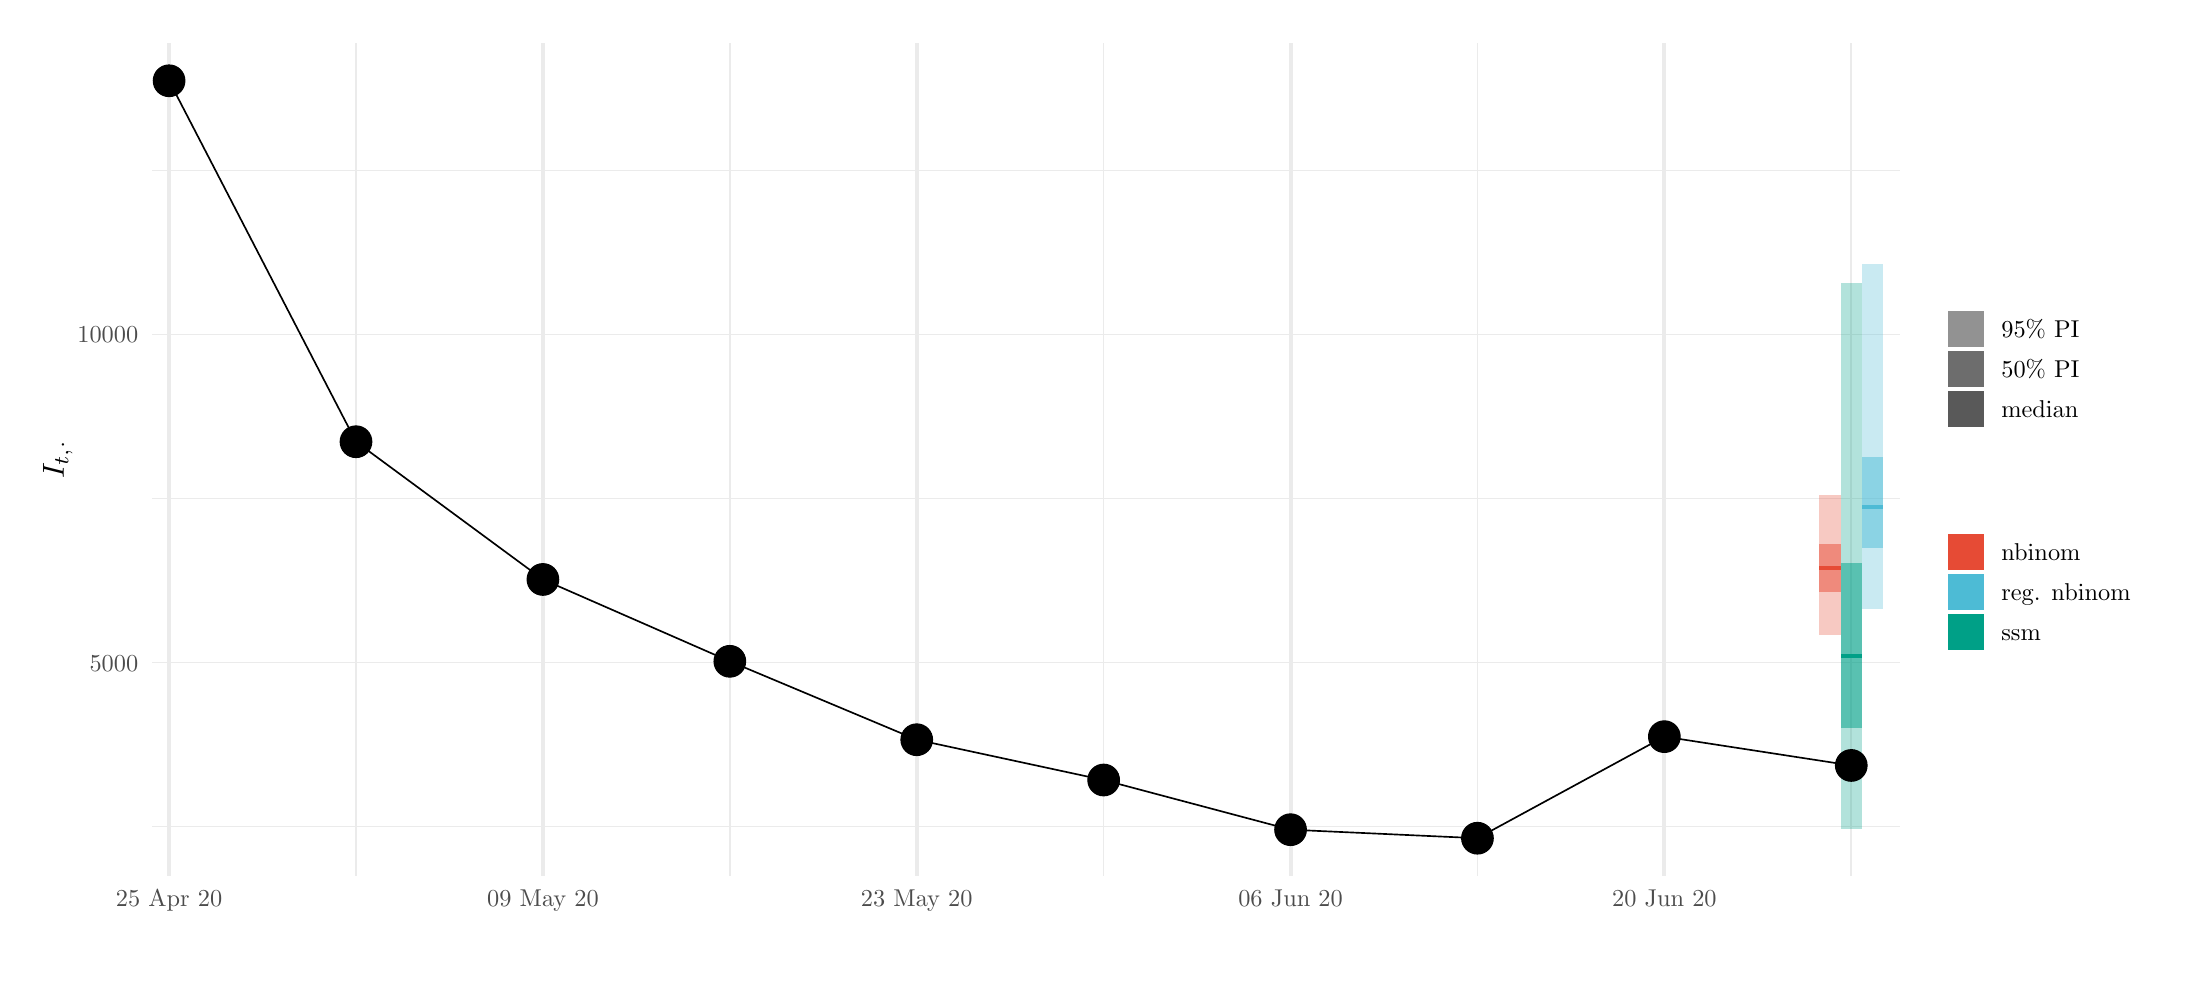
\begin{tikzpicture}[x=1pt,y=1pt]
\definecolor{fillColor}{RGB}{255,255,255}
\path[use as bounding box,fill=fillColor,fill opacity=0.00] (0,0) rectangle (770.88,337.26);
\begin{scope}
\path[clip] ( 44.91, 30.69) rectangle (676.72,331.76);
\definecolor{drawColor}{gray}{0.92}

\path[draw=drawColor,line width= 0.3pt,line join=round] ( 44.91, 48.54) --
	(676.72, 48.54);

\path[draw=drawColor,line width= 0.3pt,line join=round] ( 44.91,167.08) --
	(676.72,167.08);

\path[draw=drawColor,line width= 0.3pt,line join=round] ( 44.91,285.62) --
	(676.72,285.62);

\path[draw=drawColor,line width= 0.6pt,line join=round] (118.64, 30.69) --
	(118.64,331.76);

\path[draw=drawColor,line width= 0.6pt,line join=round] (253.72, 30.69) --
	(253.72,331.76);

\path[draw=drawColor,line width= 0.6pt,line join=round] (388.80, 30.69) --
	(388.80,331.76);

\path[draw=drawColor,line width= 0.6pt,line join=round] (523.87, 30.69) --
	(523.87,331.76);

\path[draw=drawColor,line width= 0.6pt,line join=round] (658.95, 30.69) --
	(658.95,331.76);

\path[draw=drawColor,line width= 0.6pt,line join=round] ( 44.91,107.81) --
	(676.72,107.81);

\path[draw=drawColor,line width= 0.6pt,line join=round] ( 44.91,226.35) --
	(676.72,226.35);

\path[draw=drawColor,line width= 1.4pt,line join=round] ( 51.10, 30.69) --
	( 51.10,331.76);

\path[draw=drawColor,line width= 1.4pt,line join=round] (186.18, 30.69) --
	(186.18,331.76);

\path[draw=drawColor,line width= 1.4pt,line join=round] (321.26, 30.69) --
	(321.26,331.76);

\path[draw=drawColor,line width= 1.4pt,line join=round] (456.34, 30.69) --
	(456.34,331.76);

\path[draw=drawColor,line width= 1.4pt,line join=round] (591.41, 30.69) --
	(591.41,331.76);
\definecolor{fillColor}{RGB}{0,160,135}

\path[fill=fillColor,fill opacity=0.30] (655.09, 47.61) rectangle (662.81,245.08);
\definecolor{fillColor}{RGB}{0,160,135}

\path[fill=fillColor,fill opacity=0.50] (655.09, 84.26) rectangle (662.81,143.93);
\definecolor{fillColor}{RGB}{0,160,135}

\path[fill=fillColor] (655.09,109.38) rectangle (662.81,110.80);
\definecolor{fillColor}{RGB}{230,75,53}

\path[fill=fillColor,fill opacity=0.30] (647.37,117.91) rectangle (655.09,168.55);
\definecolor{fillColor}{RGB}{230,75,53}

\path[fill=fillColor,fill opacity=0.50] (647.37,133.32) rectangle (655.09,150.72);
\definecolor{fillColor}{RGB}{230,75,53}

\path[fill=fillColor] (647.37,141.15) rectangle (655.09,142.57);
\definecolor{fillColor}{RGB}{77,187,213}

\path[fill=fillColor,fill opacity=0.30] (662.81,127.37) rectangle (670.53,251.74);
\definecolor{fillColor}{RGB}{77,187,213}

\path[fill=fillColor,fill opacity=0.50] (662.81,149.30) rectangle (670.53,182.06);
\definecolor{fillColor}{RGB}{77,187,213}

\path[fill=fillColor] (662.81,163.31) rectangle (670.53,164.73);
\definecolor{drawColor}{RGB}{0,0,0}

\path[draw=drawColor,line width= 0.6pt,line join=round] ( 51.10,318.07) --
	(118.64,187.64) --
	(186.18,137.87) --
	(253.72,108.29) --
	(321.26, 79.96) --
	(388.80, 65.40) --
	(456.34, 47.45) --
	(523.87, 44.37) --
	(591.41, 81.07) --
	(658.95, 70.66);
\definecolor{fillColor}{RGB}{0,0,0}

\path[draw=drawColor,line width= 0.4pt,line join=round,line cap=round,fill=fillColor] ( 51.10,318.07) circle (  5.71);

\path[draw=drawColor,line width= 0.4pt,line join=round,line cap=round,fill=fillColor] (118.64,187.64) circle (  5.71);

\path[draw=drawColor,line width= 0.4pt,line join=round,line cap=round,fill=fillColor] (186.18,137.87) circle (  5.71);

\path[draw=drawColor,line width= 0.4pt,line join=round,line cap=round,fill=fillColor] (253.72,108.29) circle (  5.71);

\path[draw=drawColor,line width= 0.4pt,line join=round,line cap=round,fill=fillColor] (321.26, 79.96) circle (  5.71);

\path[draw=drawColor,line width= 0.4pt,line join=round,line cap=round,fill=fillColor] (388.80, 65.40) circle (  5.71);

\path[draw=drawColor,line width= 0.4pt,line join=round,line cap=round,fill=fillColor] (456.34, 47.45) circle (  5.71);

\path[draw=drawColor,line width= 0.4pt,line join=round,line cap=round,fill=fillColor] (523.87, 44.37) circle (  5.71);

\path[draw=drawColor,line width= 0.4pt,line join=round,line cap=round,fill=fillColor] (591.41, 81.07) circle (  5.71);

\path[draw=drawColor,line width= 0.4pt,line join=round,line cap=round,fill=fillColor] (658.95, 70.66) circle (  5.71);
\end{scope}
\begin{scope}
\path[clip] (  0.00,  0.00) rectangle (770.88,337.26);
\definecolor{drawColor}{gray}{0.30}

\node[text=drawColor,anchor=base east,inner sep=0pt, outer sep=0pt, scale=  0.88] at ( 39.96,104.78) {5000};

\node[text=drawColor,anchor=base east,inner sep=0pt, outer sep=0pt, scale=  0.88] at ( 39.96,223.32) {10000};
\end{scope}
\begin{scope}
\path[clip] (  0.00,  0.00) rectangle (770.88,337.26);
\definecolor{drawColor}{gray}{0.30}

\node[text=drawColor,anchor=base,inner sep=0pt, outer sep=0pt, scale=  0.88] at ( 51.10, 19.68) {25 Apr 20};

\node[text=drawColor,anchor=base,inner sep=0pt, outer sep=0pt, scale=  0.88] at (186.18, 19.68) {09 May 20};

\node[text=drawColor,anchor=base,inner sep=0pt, outer sep=0pt, scale=  0.88] at (321.26, 19.68) {23 May 20};

\node[text=drawColor,anchor=base,inner sep=0pt, outer sep=0pt, scale=  0.88] at (456.34, 19.68) {06 Jun 20};

\node[text=drawColor,anchor=base,inner sep=0pt, outer sep=0pt, scale=  0.88] at (591.41, 19.68) {20 Jun 20};
\end{scope}
\begin{scope}
\path[clip] (  0.00,  0.00) rectangle (770.88,337.26);
\definecolor{drawColor}{RGB}{0,0,0}

\node[text=drawColor,rotate= 90.00,anchor=base,inner sep=0pt, outer sep=0pt, scale=  1.10] at ( 13.08,181.22) {$I_{t, \cdot}$};
\end{scope}
\begin{scope}
\path[clip] (  0.00,  0.00) rectangle (770.88,337.26);
\definecolor{fillColor}{RGB}{89,89,89}

\path[fill=fillColor,fill opacity=0.30] (693.94,221.84) rectangle (706.97,234.87);
\end{scope}
\begin{scope}
\path[clip] (  0.00,  0.00) rectangle (770.88,337.26);
\definecolor{fillColor}{RGB}{89,89,89}

\path[fill=fillColor,fill opacity=0.30] (693.94,221.84) rectangle (706.97,234.87);
\end{scope}
\begin{scope}
\path[clip] (  0.00,  0.00) rectangle (770.88,337.26);
\definecolor{fillColor}{RGB}{89,89,89}

\path[fill=fillColor,fill opacity=0.30] (693.94,221.84) rectangle (706.97,234.87);
\end{scope}
\begin{scope}
\path[clip] (  0.00,  0.00) rectangle (770.88,337.26);
\definecolor{fillColor}{RGB}{89,89,89}

\path[fill=fillColor,fill opacity=0.50] (693.94,207.39) rectangle (706.97,220.42);
\end{scope}
\begin{scope}
\path[clip] (  0.00,  0.00) rectangle (770.88,337.26);
\definecolor{fillColor}{RGB}{89,89,89}

\path[fill=fillColor,fill opacity=0.50] (693.94,207.39) rectangle (706.97,220.42);
\end{scope}
\begin{scope}
\path[clip] (  0.00,  0.00) rectangle (770.88,337.26);
\definecolor{fillColor}{RGB}{89,89,89}

\path[fill=fillColor,fill opacity=0.50] (693.94,207.39) rectangle (706.97,220.42);
\end{scope}
\begin{scope}
\path[clip] (  0.00,  0.00) rectangle (770.88,337.26);
\definecolor{fillColor}{gray}{0.35}

\path[fill=fillColor] (693.94,192.93) rectangle (706.97,205.97);
\end{scope}
\begin{scope}
\path[clip] (  0.00,  0.00) rectangle (770.88,337.26);
\definecolor{fillColor}{gray}{0.35}

\path[fill=fillColor] (693.94,192.93) rectangle (706.97,205.97);
\end{scope}
\begin{scope}
\path[clip] (  0.00,  0.00) rectangle (770.88,337.26);
\definecolor{fillColor}{gray}{0.35}

\path[fill=fillColor] (693.94,192.93) rectangle (706.97,205.97);
\end{scope}
\begin{scope}
\path[clip] (  0.00,  0.00) rectangle (770.88,337.26);
\definecolor{drawColor}{RGB}{0,0,0}

\node[text=drawColor,anchor=base west,inner sep=0pt, outer sep=0pt, scale=  0.88] at (713.18,225.33) {$95 \%$ PI};
\end{scope}
\begin{scope}
\path[clip] (  0.00,  0.00) rectangle (770.88,337.26);
\definecolor{drawColor}{RGB}{0,0,0}

\node[text=drawColor,anchor=base west,inner sep=0pt, outer sep=0pt, scale=  0.88] at (713.18,210.87) {$50 \%$ PI};
\end{scope}
\begin{scope}
\path[clip] (  0.00,  0.00) rectangle (770.88,337.26);
\definecolor{drawColor}{RGB}{0,0,0}

\node[text=drawColor,anchor=base west,inner sep=0pt, outer sep=0pt, scale=  0.88] at (713.18,196.42) {median};
\end{scope}
\begin{scope}
\path[clip] (  0.00,  0.00) rectangle (770.88,337.26);
\definecolor{fillColor}{RGB}{230,75,53}

\path[fill=fillColor] (693.94,141.27) rectangle (706.97,154.30);
\end{scope}
\begin{scope}
\path[clip] (  0.00,  0.00) rectangle (770.88,337.26);
\definecolor{fillColor}{RGB}{230,75,53}

\path[fill=fillColor] (693.94,141.27) rectangle (706.97,154.30);
\end{scope}
\begin{scope}
\path[clip] (  0.00,  0.00) rectangle (770.88,337.26);
\definecolor{fillColor}{RGB}{230,75,53}

\path[fill=fillColor] (693.94,141.27) rectangle (706.97,154.30);
\end{scope}
\begin{scope}
\path[clip] (  0.00,  0.00) rectangle (770.88,337.26);
\definecolor{fillColor}{RGB}{77,187,213}

\path[fill=fillColor] (693.94,126.81) rectangle (706.97,139.84);
\end{scope}
\begin{scope}
\path[clip] (  0.00,  0.00) rectangle (770.88,337.26);
\definecolor{fillColor}{RGB}{77,187,213}

\path[fill=fillColor] (693.94,126.81) rectangle (706.97,139.84);
\end{scope}
\begin{scope}
\path[clip] (  0.00,  0.00) rectangle (770.88,337.26);
\definecolor{fillColor}{RGB}{77,187,213}

\path[fill=fillColor] (693.94,126.81) rectangle (706.97,139.84);
\end{scope}
\begin{scope}
\path[clip] (  0.00,  0.00) rectangle (770.88,337.26);
\definecolor{fillColor}{RGB}{0,160,135}

\path[fill=fillColor] (693.94,112.36) rectangle (706.97,125.39);
\end{scope}
\begin{scope}
\path[clip] (  0.00,  0.00) rectangle (770.88,337.26);
\definecolor{fillColor}{RGB}{0,160,135}

\path[fill=fillColor] (693.94,112.36) rectangle (706.97,125.39);
\end{scope}
\begin{scope}
\path[clip] (  0.00,  0.00) rectangle (770.88,337.26);
\definecolor{fillColor}{RGB}{0,160,135}

\path[fill=fillColor] (693.94,112.36) rectangle (706.97,125.39);
\end{scope}
\begin{scope}
\path[clip] (  0.00,  0.00) rectangle (770.88,337.26);
\definecolor{drawColor}{RGB}{0,0,0}

\node[text=drawColor,anchor=base west,inner sep=0pt, outer sep=0pt, scale=  0.88] at (713.18,144.75) {nbinom};
\end{scope}
\begin{scope}
\path[clip] (  0.00,  0.00) rectangle (770.88,337.26);
\definecolor{drawColor}{RGB}{0,0,0}

\node[text=drawColor,anchor=base west,inner sep=0pt, outer sep=0pt, scale=  0.88] at (713.18,130.30) {reg. nbinom};
\end{scope}
\begin{scope}
\path[clip] (  0.00,  0.00) rectangle (770.88,337.26);
\definecolor{drawColor}{RGB}{0,0,0}

\node[text=drawColor,anchor=base west,inner sep=0pt, outer sep=0pt, scale=  0.88] at (713.18,115.84) {ssm};
\end{scope}
\end{tikzpicture}
%
    }
    \caption{Incidences $I_{t,\cdot} = \sum_{r = 1}^R I_{t,r}$ in Germany in the period under consideration in the regional showcase model. We additionally show predictions (median, $80\%$ and $95\%$ prediction intervals) as shaded regions for three different approaches: the \acrshort{ssm} presented in this section and two negative binomial baselines (see text for details). The \acrshort{ssm} approach is the only approach with the actual incidences ending up within the $80\%$ prediction interval, the two baselines completely miss this target.}
    \label{fig:regional_showcase_prediction.tex}
\end{figure}

\begin{figure}
    \resizebox{\textwidth}{!}{%
        % Created by tikzDevice version 0.12.6 on 2025-09-21 16:35:02
% !TEX encoding = UTF-8 Unicode
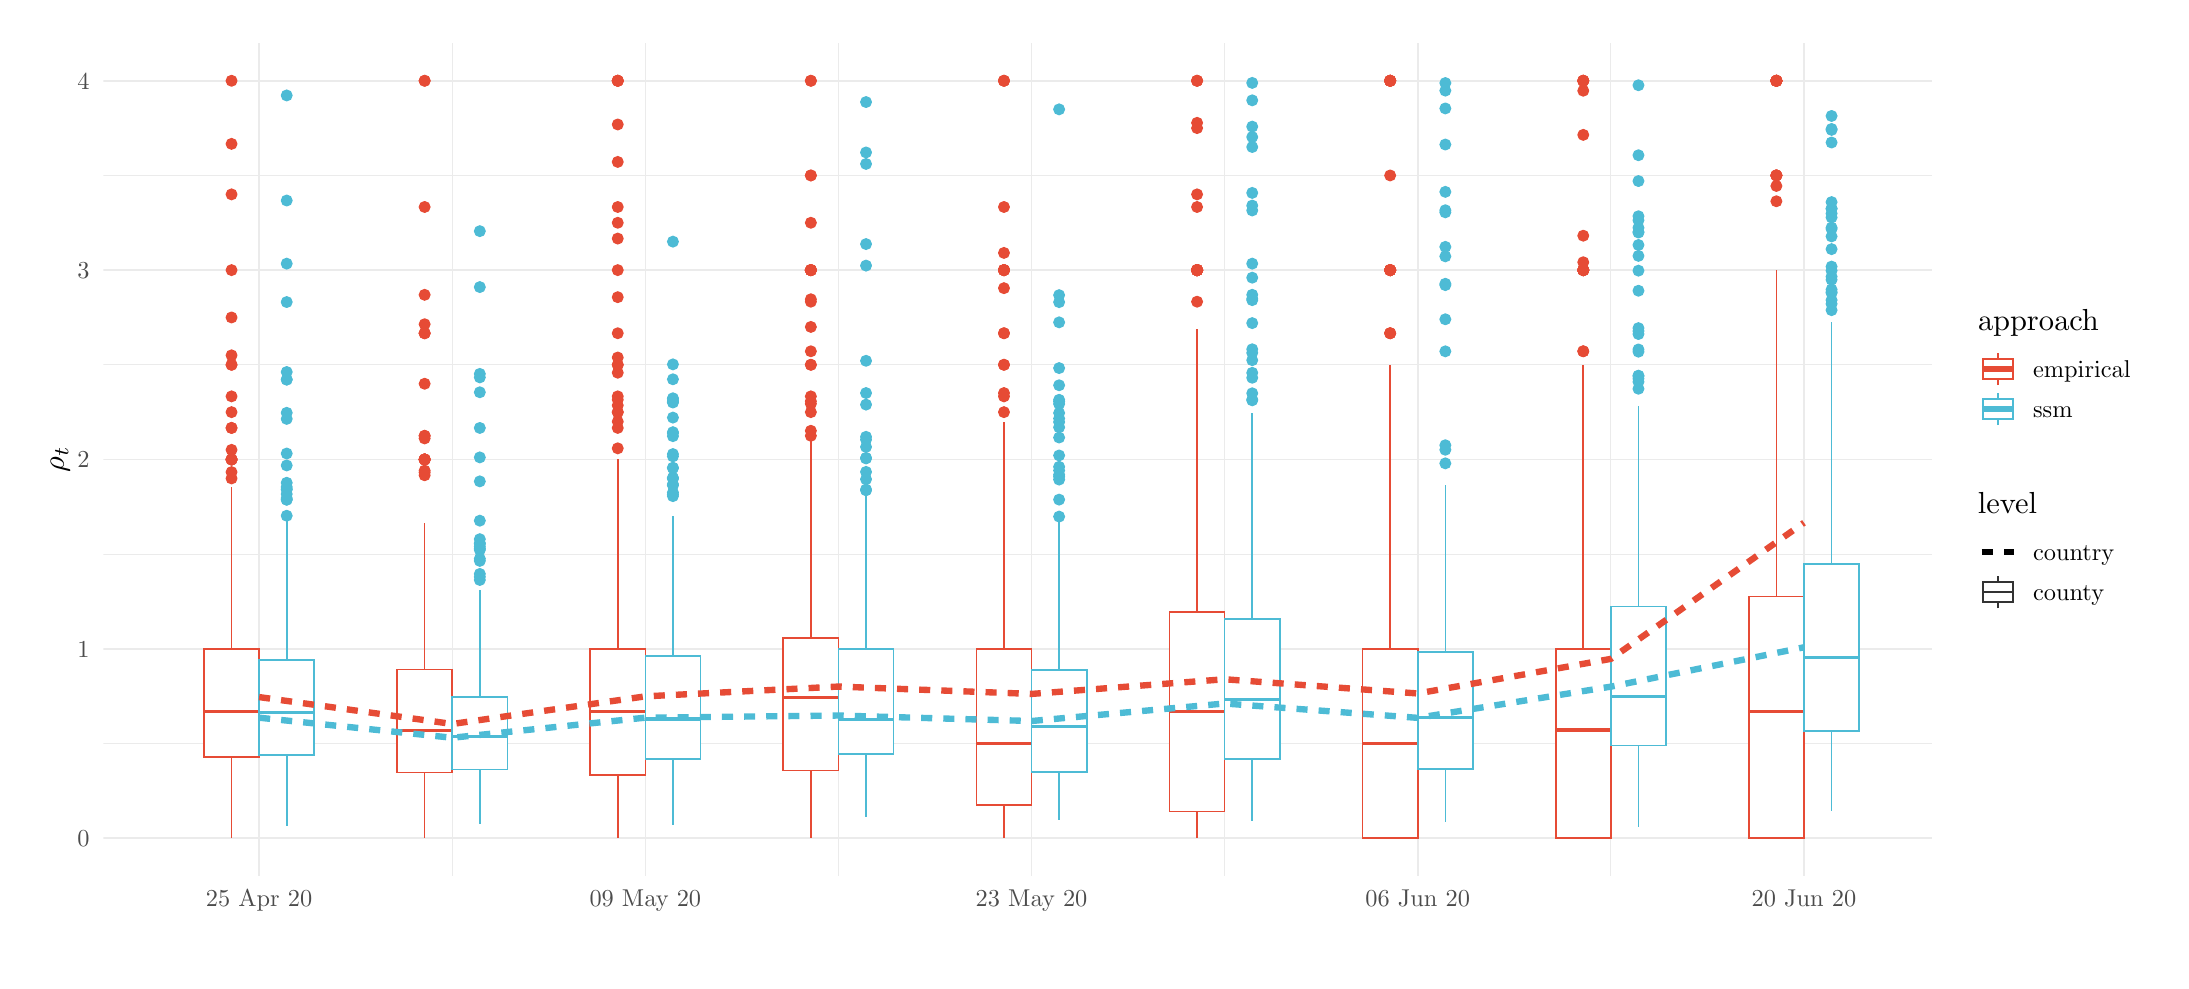
\begin{tikzpicture}[x=1pt,y=1pt]
\definecolor{fillColor}{RGB}{255,255,255}
\path[use as bounding box,fill=fillColor,fill opacity=0.00] (0,0) rectangle (770.88,337.26);
\begin{scope}
\path[clip] ( 27.31, 30.69) rectangle (688.21,331.76);
\definecolor{drawColor}{gray}{0.92}

\path[draw=drawColor,line width= 0.3pt,line join=round] ( 27.31, 78.58) --
	(688.21, 78.58);

\path[draw=drawColor,line width= 0.3pt,line join=round] ( 27.31,147.01) --
	(688.21,147.01);

\path[draw=drawColor,line width= 0.3pt,line join=round] ( 27.31,215.44) --
	(688.21,215.44);

\path[draw=drawColor,line width= 0.3pt,line join=round] ( 27.31,283.86) --
	(688.21,283.86);

\path[draw=drawColor,line width= 0.3pt,line join=round] (153.41, 30.69) --
	(153.41,331.76);

\path[draw=drawColor,line width= 0.3pt,line join=round] (292.97, 30.69) --
	(292.97,331.76);

\path[draw=drawColor,line width= 0.3pt,line join=round] (432.52, 30.69) --
	(432.52,331.76);

\path[draw=drawColor,line width= 0.3pt,line join=round] (572.08, 30.69) --
	(572.08,331.76);

\path[draw=drawColor,line width= 0.6pt,line join=round] ( 27.31, 44.37) --
	(688.21, 44.37);

\path[draw=drawColor,line width= 0.6pt,line join=round] ( 27.31,112.80) --
	(688.21,112.80);

\path[draw=drawColor,line width= 0.6pt,line join=round] ( 27.31,181.22) --
	(688.21,181.22);

\path[draw=drawColor,line width= 0.6pt,line join=round] ( 27.31,249.65) --
	(688.21,249.65);

\path[draw=drawColor,line width= 0.6pt,line join=round] ( 27.31,318.07) --
	(688.21,318.07);

\path[draw=drawColor,line width= 0.6pt,line join=round] ( 83.63, 30.69) --
	( 83.63,331.76);

\path[draw=drawColor,line width= 0.6pt,line join=round] (223.19, 30.69) --
	(223.19,331.76);

\path[draw=drawColor,line width= 0.6pt,line join=round] (362.75, 30.69) --
	(362.75,331.76);

\path[draw=drawColor,line width= 0.6pt,line join=round] (502.30, 30.69) --
	(502.30,331.76);

\path[draw=drawColor,line width= 0.6pt,line join=round] (641.86, 30.69) --
	(641.86,331.76);
\definecolor{drawColor}{RGB}{230,75,53}
\definecolor{fillColor}{RGB}{230,75,53}

\path[draw=drawColor,line width= 0.4pt,line join=round,line cap=round,fill=fillColor] ( 73.67,215.44) circle (  1.96);

\path[draw=drawColor,line width= 0.4pt,line join=round,line cap=round,fill=fillColor] ( 73.67,277.02) circle (  1.96);

\path[draw=drawColor,line width= 0.4pt,line join=round,line cap=round,fill=fillColor] ( 73.67,181.22) circle (  1.96);

\path[draw=drawColor,line width= 0.4pt,line join=round,line cap=round,fill=fillColor] ( 73.67,181.22) circle (  1.96);

\path[draw=drawColor,line width= 0.4pt,line join=round,line cap=round,fill=fillColor] ( 73.67,184.70) circle (  1.96);

\path[draw=drawColor,line width= 0.4pt,line join=round,line cap=round,fill=fillColor] ( 73.67,218.86) circle (  1.96);

\path[draw=drawColor,line width= 0.4pt,line join=round,line cap=round,fill=fillColor] ( 73.67,192.63) circle (  1.96);

\path[draw=drawColor,line width= 0.4pt,line join=round,line cap=round,fill=fillColor] ( 73.67,215.44) circle (  1.96);

\path[draw=drawColor,line width= 0.4pt,line join=round,line cap=round,fill=fillColor] ( 73.67,192.63) circle (  1.96);

\path[draw=drawColor,line width= 0.4pt,line join=round,line cap=round,fill=fillColor] ( 73.67,181.22) circle (  1.96);

\path[draw=drawColor,line width= 0.4pt,line join=round,line cap=round,fill=fillColor] ( 73.67,174.38) circle (  1.96);

\path[draw=drawColor,line width= 0.4pt,line join=round,line cap=round,fill=fillColor] ( 73.67,295.27) circle (  1.96);

\path[draw=drawColor,line width= 0.4pt,line join=round,line cap=round,fill=fillColor] ( 73.67,232.54) circle (  1.96);

\path[draw=drawColor,line width= 0.4pt,line join=round,line cap=round,fill=fillColor] ( 73.67,176.66) circle (  1.96);

\path[draw=drawColor,line width= 0.4pt,line join=round,line cap=round,fill=fillColor] ( 73.67,204.03) circle (  1.96);

\path[draw=drawColor,line width= 0.4pt,line join=round,line cap=round,fill=fillColor] ( 73.67,181.22) circle (  1.96);

\path[draw=drawColor,line width= 0.4pt,line join=round,line cap=round,fill=fillColor] ( 73.67,181.22) circle (  1.96);

\path[draw=drawColor,line width= 0.4pt,line join=round,line cap=round,fill=fillColor] ( 73.67,249.65) circle (  1.96);

\path[draw=drawColor,line width= 0.4pt,line join=round,line cap=round,fill=fillColor] ( 73.67,198.33) circle (  1.96);

\path[draw=drawColor,line width= 0.4pt,line join=round,line cap=round,fill=fillColor] ( 73.67,318.07) circle (  1.96);

\path[draw=drawColor,line width= 0.6pt,line join=round] ( 73.67,112.80) -- ( 73.67,171.45);

\path[draw=drawColor,line width= 0.6pt,line join=round] ( 73.67, 73.70) -- ( 73.67, 44.37);
\definecolor{fillColor}{RGB}{255,255,255}

\path[draw=drawColor,line width= 0.6pt,fill=fillColor] ( 63.70,112.80) --
	( 63.70, 73.70) --
	( 83.63, 73.70) --
	( 83.63,112.80) --
	( 63.70,112.80) --
	cycle;

\path[draw=drawColor,line width= 1.1pt] ( 63.70, 89.99) -- ( 83.63, 89.99);
\definecolor{fillColor}{RGB}{230,75,53}

\path[draw=drawColor,line width= 0.4pt,line join=round,line cap=round,fill=fillColor] (143.44,208.59) circle (  1.96);

\path[draw=drawColor,line width= 0.4pt,line join=round,line cap=round,fill=fillColor] (143.44,181.22) circle (  1.96);

\path[draw=drawColor,line width= 0.4pt,line join=round,line cap=round,fill=fillColor] (143.44,318.07) circle (  1.96);

\path[draw=drawColor,line width= 0.4pt,line join=round,line cap=round,fill=fillColor] (143.44,226.84) circle (  1.96);

\path[draw=drawColor,line width= 0.4pt,line join=round,line cap=round,fill=fillColor] (143.44,226.84) circle (  1.96);

\path[draw=drawColor,line width= 0.4pt,line join=round,line cap=round,fill=fillColor] (143.44,177.20) circle (  1.96);

\path[draw=drawColor,line width= 0.4pt,line join=round,line cap=round,fill=fillColor] (143.44,272.46) circle (  1.96);

\path[draw=drawColor,line width= 0.4pt,line join=round,line cap=round,fill=fillColor] (143.44,188.83) circle (  1.96);

\path[draw=drawColor,line width= 0.4pt,line join=round,line cap=round,fill=fillColor] (143.44,175.52) circle (  1.96);

\path[draw=drawColor,line width= 0.4pt,line join=round,line cap=round,fill=fillColor] (143.44,181.22) circle (  1.96);

\path[draw=drawColor,line width= 0.4pt,line join=round,line cap=round,fill=fillColor] (143.44,240.72) circle (  1.96);

\path[draw=drawColor,line width= 0.4pt,line join=round,line cap=round,fill=fillColor] (143.44,176.50) circle (  1.96);

\path[draw=drawColor,line width= 0.4pt,line join=round,line cap=round,fill=fillColor] (143.44,226.84) circle (  1.96);

\path[draw=drawColor,line width= 0.4pt,line join=round,line cap=round,fill=fillColor] (143.44,189.78) circle (  1.96);

\path[draw=drawColor,line width= 0.4pt,line join=round,line cap=round,fill=fillColor] (143.44,230.10) circle (  1.96);

\path[draw=drawColor,line width= 0.4pt,line join=round,line cap=round,fill=fillColor] (143.44,318.07) circle (  1.96);

\path[draw=drawColor,line width= 0.4pt,line join=round,line cap=round,fill=fillColor] (143.44,181.22) circle (  1.96);

\path[draw=drawColor,line width= 0.4pt,line join=round,line cap=round,fill=fillColor] (143.44,181.22) circle (  1.96);

\path[draw=drawColor,line width= 0.4pt,line join=round,line cap=round,fill=fillColor] (143.44,181.22) circle (  1.96);

\path[draw=drawColor,line width= 0.4pt,line join=round,line cap=round,fill=fillColor] (143.44,181.22) circle (  1.96);

\path[draw=drawColor,line width= 0.4pt,line join=round,line cap=round,fill=fillColor] (143.44,189.78) circle (  1.96);

\path[draw=drawColor,line width= 0.4pt,line join=round,line cap=round,fill=fillColor] (143.44,181.22) circle (  1.96);

\path[draw=drawColor,line width= 0.4pt,line join=round,line cap=round,fill=fillColor] (143.44,181.22) circle (  1.96);

\path[draw=drawColor,line width= 0.6pt,line join=round] (143.44,105.38) -- (143.44,158.41);

\path[draw=drawColor,line width= 0.6pt,line join=round] (143.44, 68.17) -- (143.44, 44.37);
\definecolor{fillColor}{RGB}{255,255,255}

\path[draw=drawColor,line width= 0.6pt,fill=fillColor] (133.48,105.38) --
	(133.48, 68.17) --
	(153.41, 68.17) --
	(153.41,105.38) --
	(133.48,105.38) --
	cycle;

\path[draw=drawColor,line width= 1.1pt] (133.48, 83.36) -- (153.41, 83.36);
\definecolor{fillColor}{RGB}{230,75,53}

\path[draw=drawColor,line width= 0.4pt,line join=round,line cap=round,fill=fillColor] (213.22,249.65) circle (  1.96);

\path[draw=drawColor,line width= 0.4pt,line join=round,line cap=round,fill=fillColor] (213.22,261.05) circle (  1.96);

\path[draw=drawColor,line width= 0.4pt,line join=round,line cap=round,fill=fillColor] (213.22,185.25) circle (  1.96);

\path[draw=drawColor,line width= 0.4pt,line join=round,line cap=round,fill=fillColor] (213.22,302.28) circle (  1.96);

\path[draw=drawColor,line width= 0.4pt,line join=round,line cap=round,fill=fillColor] (213.22,318.07) circle (  1.96);

\path[draw=drawColor,line width= 0.4pt,line join=round,line cap=round,fill=fillColor] (213.22,215.44) circle (  1.96);

\path[draw=drawColor,line width= 0.4pt,line join=round,line cap=round,fill=fillColor] (213.22,212.58) circle (  1.96);

\path[draw=drawColor,line width= 0.4pt,line join=round,line cap=round,fill=fillColor] (213.22,272.46) circle (  1.96);

\path[draw=drawColor,line width= 0.4pt,line join=round,line cap=round,fill=fillColor] (213.22,194.91) circle (  1.96);

\path[draw=drawColor,line width= 0.4pt,line join=round,line cap=round,fill=fillColor] (213.22,198.33) circle (  1.96);

\path[draw=drawColor,line width= 0.4pt,line join=round,line cap=round,fill=fillColor] (213.22,192.63) circle (  1.96);

\path[draw=drawColor,line width= 0.4pt,line join=round,line cap=round,fill=fillColor] (213.22,218.07) circle (  1.96);

\path[draw=drawColor,line width= 0.4pt,line join=round,line cap=round,fill=fillColor] (213.22,266.76) circle (  1.96);

\path[draw=drawColor,line width= 0.4pt,line join=round,line cap=round,fill=fillColor] (213.22,288.75) circle (  1.96);

\path[draw=drawColor,line width= 0.4pt,line join=round,line cap=round,fill=fillColor] (213.22,318.07) circle (  1.96);

\path[draw=drawColor,line width= 0.4pt,line join=round,line cap=round,fill=fillColor] (213.22,198.33) circle (  1.96);

\path[draw=drawColor,line width= 0.4pt,line join=round,line cap=round,fill=fillColor] (213.22,204.03) circle (  1.96);

\path[draw=drawColor,line width= 0.4pt,line join=round,line cap=round,fill=fillColor] (213.22,202.83) circle (  1.96);

\path[draw=drawColor,line width= 0.4pt,line join=round,line cap=round,fill=fillColor] (213.22,239.87) circle (  1.96);

\path[draw=drawColor,line width= 0.4pt,line join=round,line cap=round,fill=fillColor] (213.22,226.84) circle (  1.96);

\path[draw=drawColor,line width= 0.4pt,line join=round,line cap=round,fill=fillColor] (213.22,318.07) circle (  1.96);

\path[draw=drawColor,line width= 0.4pt,line join=round,line cap=round,fill=fillColor] (213.22,200.77) circle (  1.96);

\path[draw=drawColor,line width= 0.4pt,line join=round,line cap=round,fill=fillColor] (213.22,318.07) circle (  1.96);

\path[draw=drawColor,line width= 0.4pt,line join=round,line cap=round,fill=fillColor] (213.22,215.44) circle (  1.96);

\path[draw=drawColor,line width= 0.4pt,line join=round,line cap=round,fill=fillColor] (213.22,318.07) circle (  1.96);

\path[draw=drawColor,line width= 0.6pt,line join=round] (213.22,112.80) -- (213.22,181.22);

\path[draw=drawColor,line width= 0.6pt,line join=round] (213.22, 67.18) -- (213.22, 44.37);
\definecolor{fillColor}{RGB}{255,255,255}

\path[draw=drawColor,line width= 0.6pt,fill=fillColor] (203.25,112.80) --
	(203.25, 67.18) --
	(223.19, 67.18) --
	(223.19,112.80) --
	(203.25,112.80) --
	cycle;

\path[draw=drawColor,line width= 1.1pt] (203.25, 89.99) -- (223.19, 89.99);
\definecolor{fillColor}{RGB}{230,75,53}

\path[draw=drawColor,line width= 0.4pt,line join=round,line cap=round,fill=fillColor] (283.00,249.65) circle (  1.96);

\path[draw=drawColor,line width= 0.4pt,line join=round,line cap=round,fill=fillColor] (283.00,249.65) circle (  1.96);

\path[draw=drawColor,line width= 0.4pt,line join=round,line cap=round,fill=fillColor] (283.00,318.07) circle (  1.96);

\path[draw=drawColor,line width= 0.4pt,line join=round,line cap=round,fill=fillColor] (283.00,239.12) circle (  1.96);

\path[draw=drawColor,line width= 0.4pt,line join=round,line cap=round,fill=fillColor] (283.00,202.28) circle (  1.96);

\path[draw=drawColor,line width= 0.4pt,line join=round,line cap=round,fill=fillColor] (283.00,191.59) circle (  1.96);

\path[draw=drawColor,line width= 0.4pt,line join=round,line cap=round,fill=fillColor] (283.00,266.76) circle (  1.96);

\path[draw=drawColor,line width= 0.4pt,line join=round,line cap=round,fill=fillColor] (283.00,238.24) circle (  1.96);

\path[draw=drawColor,line width= 0.4pt,line join=round,line cap=round,fill=fillColor] (283.00,220.32) circle (  1.96);

\path[draw=drawColor,line width= 0.4pt,line join=round,line cap=round,fill=fillColor] (283.00,215.44) circle (  1.96);

\path[draw=drawColor,line width= 0.4pt,line join=round,line cap=round,fill=fillColor] (283.00,249.65) circle (  1.96);

\path[draw=drawColor,line width= 0.4pt,line join=round,line cap=round,fill=fillColor] (283.00,318.07) circle (  1.96);

\path[draw=drawColor,line width= 0.4pt,line join=round,line cap=round,fill=fillColor] (283.00,215.44) circle (  1.96);

\path[draw=drawColor,line width= 0.4pt,line join=round,line cap=round,fill=fillColor] (283.00,201.35) circle (  1.96);

\path[draw=drawColor,line width= 0.4pt,line join=round,line cap=round,fill=fillColor] (283.00,249.65) circle (  1.96);

\path[draw=drawColor,line width= 0.4pt,line join=round,line cap=round,fill=fillColor] (283.00,229.12) circle (  1.96);

\path[draw=drawColor,line width= 0.4pt,line join=round,line cap=round,fill=fillColor] (283.00,198.33) circle (  1.96);

\path[draw=drawColor,line width= 0.4pt,line join=round,line cap=round,fill=fillColor] (283.00,283.86) circle (  1.96);

\path[draw=drawColor,line width= 0.4pt,line join=round,line cap=round,fill=fillColor] (283.00,204.03) circle (  1.96);

\path[draw=drawColor,line width= 0.4pt,line join=round,line cap=round,fill=fillColor] (283.00,189.78) circle (  1.96);

\path[draw=drawColor,line width= 0.4pt,line join=round,line cap=round,fill=fillColor] (283.00,283.86) circle (  1.96);

\path[draw=drawColor,line width= 0.4pt,line join=round,line cap=round,fill=fillColor] (283.00,249.65) circle (  1.96);

\path[draw=drawColor,line width= 0.4pt,line join=round,line cap=round,fill=fillColor] (283.00,249.65) circle (  1.96);

\path[draw=drawColor,line width= 0.4pt,line join=round,line cap=round,fill=fillColor] (283.00,249.65) circle (  1.96);

\path[draw=drawColor,line width= 0.4pt,line join=round,line cap=round,fill=fillColor] (283.00,249.65) circle (  1.96);

\path[draw=drawColor,line width= 0.6pt,line join=round] (283.00,116.82) -- (283.00,188.07);

\path[draw=drawColor,line width= 0.6pt,line join=round] (283.00, 68.81) -- (283.00, 44.37);
\definecolor{fillColor}{RGB}{255,255,255}

\path[draw=drawColor,line width= 0.6pt,fill=fillColor] (273.03,116.82) --
	(273.03, 68.81) --
	(292.97, 68.81) --
	(292.97,116.82) --
	(273.03,116.82) --
	cycle;

\path[draw=drawColor,line width= 1.1pt] (273.03, 95.09) -- (292.97, 95.09);
\definecolor{fillColor}{RGB}{230,75,53}

\path[draw=drawColor,line width= 0.4pt,line join=round,line cap=round,fill=fillColor] (352.78,255.87) circle (  1.96);

\path[draw=drawColor,line width= 0.4pt,line join=round,line cap=round,fill=fillColor] (352.78,226.84) circle (  1.96);

\path[draw=drawColor,line width= 0.4pt,line join=round,line cap=round,fill=fillColor] (352.78,249.65) circle (  1.96);

\path[draw=drawColor,line width= 0.4pt,line join=round,line cap=round,fill=fillColor] (352.78,249.65) circle (  1.96);

\path[draw=drawColor,line width= 0.4pt,line join=round,line cap=round,fill=fillColor] (352.78,205.23) circle (  1.96);

\path[draw=drawColor,line width= 0.4pt,line join=round,line cap=round,fill=fillColor] (352.78,249.65) circle (  1.96);

\path[draw=drawColor,line width= 0.4pt,line join=round,line cap=round,fill=fillColor] (352.78,272.46) circle (  1.96);

\path[draw=drawColor,line width= 0.4pt,line join=round,line cap=round,fill=fillColor] (352.78,215.44) circle (  1.96);

\path[draw=drawColor,line width= 0.4pt,line join=round,line cap=round,fill=fillColor] (352.78,215.44) circle (  1.96);

\path[draw=drawColor,line width= 0.4pt,line join=round,line cap=round,fill=fillColor] (352.78,243.13) circle (  1.96);

\path[draw=drawColor,line width= 0.4pt,line join=round,line cap=round,fill=fillColor] (352.78,318.07) circle (  1.96);

\path[draw=drawColor,line width= 0.4pt,line join=round,line cap=round,fill=fillColor] (352.78,204.03) circle (  1.96);

\path[draw=drawColor,line width= 0.4pt,line join=round,line cap=round,fill=fillColor] (352.78,198.33) circle (  1.96);

\path[draw=drawColor,line width= 0.4pt,line join=round,line cap=round,fill=fillColor] (352.78,226.84) circle (  1.96);

\path[draw=drawColor,line width= 0.4pt,line join=round,line cap=round,fill=fillColor] (352.78,249.65) circle (  1.96);

\path[draw=drawColor,line width= 0.4pt,line join=round,line cap=round,fill=fillColor] (352.78,249.65) circle (  1.96);

\path[draw=drawColor,line width= 0.4pt,line join=round,line cap=round,fill=fillColor] (352.78,318.07) circle (  1.96);

\path[draw=drawColor,line width= 0.4pt,line join=round,line cap=round,fill=fillColor] (352.78,318.07) circle (  1.96);

\path[draw=drawColor,line width= 0.4pt,line join=round,line cap=round,fill=fillColor] (352.78,249.65) circle (  1.96);

\path[draw=drawColor,line width= 0.4pt,line join=round,line cap=round,fill=fillColor] (352.78,249.65) circle (  1.96);

\path[draw=drawColor,line width= 0.4pt,line join=round,line cap=round,fill=fillColor] (352.78,249.65) circle (  1.96);

\path[draw=drawColor,line width= 0.6pt,line join=round] (352.78,112.80) -- (352.78,194.91);

\path[draw=drawColor,line width= 0.6pt,line join=round] (352.78, 56.45) -- (352.78, 44.37);
\definecolor{fillColor}{RGB}{255,255,255}

\path[draw=drawColor,line width= 0.6pt,fill=fillColor] (342.81,112.80) --
	(342.81, 56.45) --
	(362.75, 56.45) --
	(362.75,112.80) --
	(342.81,112.80) --
	cycle;

\path[draw=drawColor,line width= 1.1pt] (342.81, 78.58) -- (362.75, 78.58);
\definecolor{fillColor}{RGB}{230,75,53}

\path[draw=drawColor,line width= 0.4pt,line join=round,line cap=round,fill=fillColor] (422.56,249.65) circle (  1.96);

\path[draw=drawColor,line width= 0.4pt,line join=round,line cap=round,fill=fillColor] (422.56,249.65) circle (  1.96);

\path[draw=drawColor,line width= 0.4pt,line join=round,line cap=round,fill=fillColor] (422.56,249.65) circle (  1.96);

\path[draw=drawColor,line width= 0.4pt,line join=round,line cap=round,fill=fillColor] (422.56,249.65) circle (  1.96);

\path[draw=drawColor,line width= 0.4pt,line join=round,line cap=round,fill=fillColor] (422.56,249.65) circle (  1.96);

\path[draw=drawColor,line width= 0.4pt,line join=round,line cap=round,fill=fillColor] (422.56,300.97) circle (  1.96);

\path[draw=drawColor,line width= 0.4pt,line join=round,line cap=round,fill=fillColor] (422.56,302.87) circle (  1.96);

\path[draw=drawColor,line width= 0.4pt,line join=round,line cap=round,fill=fillColor] (422.56,238.24) circle (  1.96);

\path[draw=drawColor,line width= 0.4pt,line join=round,line cap=round,fill=fillColor] (422.56,249.65) circle (  1.96);

\path[draw=drawColor,line width= 0.4pt,line join=round,line cap=round,fill=fillColor] (422.56,249.65) circle (  1.96);

\path[draw=drawColor,line width= 0.4pt,line join=round,line cap=round,fill=fillColor] (422.56,249.65) circle (  1.96);

\path[draw=drawColor,line width= 0.4pt,line join=round,line cap=round,fill=fillColor] (422.56,249.65) circle (  1.96);

\path[draw=drawColor,line width= 0.4pt,line join=round,line cap=round,fill=fillColor] (422.56,249.65) circle (  1.96);

\path[draw=drawColor,line width= 0.4pt,line join=round,line cap=round,fill=fillColor] (422.56,249.65) circle (  1.96);

\path[draw=drawColor,line width= 0.4pt,line join=round,line cap=round,fill=fillColor] (422.56,318.07) circle (  1.96);

\path[draw=drawColor,line width= 0.4pt,line join=round,line cap=round,fill=fillColor] (422.56,249.65) circle (  1.96);

\path[draw=drawColor,line width= 0.4pt,line join=round,line cap=round,fill=fillColor] (422.56,318.07) circle (  1.96);

\path[draw=drawColor,line width= 0.4pt,line join=round,line cap=round,fill=fillColor] (422.56,249.65) circle (  1.96);

\path[draw=drawColor,line width= 0.4pt,line join=round,line cap=round,fill=fillColor] (422.56,249.65) circle (  1.96);

\path[draw=drawColor,line width= 0.4pt,line join=round,line cap=round,fill=fillColor] (422.56,249.65) circle (  1.96);

\path[draw=drawColor,line width= 0.4pt,line join=round,line cap=round,fill=fillColor] (422.56,318.07) circle (  1.96);

\path[draw=drawColor,line width= 0.4pt,line join=round,line cap=round,fill=fillColor] (422.56,249.65) circle (  1.96);

\path[draw=drawColor,line width= 0.4pt,line join=round,line cap=round,fill=fillColor] (422.56,249.65) circle (  1.96);

\path[draw=drawColor,line width= 0.4pt,line join=round,line cap=round,fill=fillColor] (422.56,249.65) circle (  1.96);

\path[draw=drawColor,line width= 0.4pt,line join=round,line cap=round,fill=fillColor] (422.56,249.65) circle (  1.96);

\path[draw=drawColor,line width= 0.4pt,line join=round,line cap=round,fill=fillColor] (422.56,277.02) circle (  1.96);

\path[draw=drawColor,line width= 0.4pt,line join=round,line cap=round,fill=fillColor] (422.56,272.46) circle (  1.96);

\path[draw=drawColor,line width= 0.6pt,line join=round] (422.56,126.15) -- (422.56,228.27);

\path[draw=drawColor,line width= 0.6pt,line join=round] (422.56, 54.07) -- (422.56, 44.37);
\definecolor{fillColor}{RGB}{255,255,255}

\path[draw=drawColor,line width= 0.6pt,fill=fillColor] (412.59,126.15) --
	(412.59, 54.07) --
	(432.52, 54.07) --
	(432.52,126.15) --
	(412.59,126.15) --
	cycle;

\path[draw=drawColor,line width= 1.1pt] (412.59, 89.99) -- (432.52, 89.99);
\definecolor{fillColor}{RGB}{230,75,53}

\path[draw=drawColor,line width= 0.4pt,line join=round,line cap=round,fill=fillColor] (492.33,318.07) circle (  1.96);

\path[draw=drawColor,line width= 0.4pt,line join=round,line cap=round,fill=fillColor] (492.33,249.65) circle (  1.96);

\path[draw=drawColor,line width= 0.4pt,line join=round,line cap=round,fill=fillColor] (492.33,283.86) circle (  1.96);

\path[draw=drawColor,line width= 0.4pt,line join=round,line cap=round,fill=fillColor] (492.33,226.84) circle (  1.96);

\path[draw=drawColor,line width= 0.4pt,line join=round,line cap=round,fill=fillColor] (492.33,318.07) circle (  1.96);

\path[draw=drawColor,line width= 0.4pt,line join=round,line cap=round,fill=fillColor] (492.33,249.65) circle (  1.96);

\path[draw=drawColor,line width= 0.4pt,line join=round,line cap=round,fill=fillColor] (492.33,249.65) circle (  1.96);

\path[draw=drawColor,line width= 0.4pt,line join=round,line cap=round,fill=fillColor] (492.33,226.84) circle (  1.96);

\path[draw=drawColor,line width= 0.4pt,line join=round,line cap=round,fill=fillColor] (492.33,318.07) circle (  1.96);

\path[draw=drawColor,line width= 0.4pt,line join=round,line cap=round,fill=fillColor] (492.33,226.84) circle (  1.96);

\path[draw=drawColor,line width= 0.4pt,line join=round,line cap=round,fill=fillColor] (492.33,318.07) circle (  1.96);

\path[draw=drawColor,line width= 0.4pt,line join=round,line cap=round,fill=fillColor] (492.33,318.07) circle (  1.96);

\path[draw=drawColor,line width= 0.4pt,line join=round,line cap=round,fill=fillColor] (492.33,318.07) circle (  1.96);

\path[draw=drawColor,line width= 0.4pt,line join=round,line cap=round,fill=fillColor] (492.33,249.65) circle (  1.96);

\path[draw=drawColor,line width= 0.4pt,line join=round,line cap=round,fill=fillColor] (492.33,249.65) circle (  1.96);

\path[draw=drawColor,line width= 0.4pt,line join=round,line cap=round,fill=fillColor] (492.33,249.65) circle (  1.96);

\path[draw=drawColor,line width= 0.4pt,line join=round,line cap=round,fill=fillColor] (492.33,249.65) circle (  1.96);

\path[draw=drawColor,line width= 0.4pt,line join=round,line cap=round,fill=fillColor] (492.33,318.07) circle (  1.96);

\path[draw=drawColor,line width= 0.4pt,line join=round,line cap=round,fill=fillColor] (492.33,318.07) circle (  1.96);

\path[draw=drawColor,line width= 0.4pt,line join=round,line cap=round,fill=fillColor] (492.33,249.65) circle (  1.96);

\path[draw=drawColor,line width= 0.4pt,line join=round,line cap=round,fill=fillColor] (492.33,249.65) circle (  1.96);

\path[draw=drawColor,line width= 0.4pt,line join=round,line cap=round,fill=fillColor] (492.33,249.65) circle (  1.96);

\path[draw=drawColor,line width= 0.6pt,line join=round] (492.33,112.80) -- (492.33,215.44);

\path[draw=drawColor,line width= 0.6pt,line join=round] (492.33, 44.37) -- (492.33, 44.37);
\definecolor{fillColor}{RGB}{255,255,255}

\path[draw=drawColor,line width= 0.6pt,fill=fillColor] (482.37,112.80) --
	(482.37, 44.37) --
	(502.30, 44.37) --
	(502.30,112.80) --
	(482.37,112.80) --
	cycle;

\path[draw=drawColor,line width= 1.1pt] (482.37, 78.58) -- (502.30, 78.58);
\definecolor{fillColor}{RGB}{230,75,53}

\path[draw=drawColor,line width= 0.4pt,line join=round,line cap=round,fill=fillColor] (562.11,249.65) circle (  1.96);

\path[draw=drawColor,line width= 0.4pt,line join=round,line cap=round,fill=fillColor] (562.11,298.52) circle (  1.96);

\path[draw=drawColor,line width= 0.4pt,line join=round,line cap=round,fill=fillColor] (562.11,249.65) circle (  1.96);

\path[draw=drawColor,line width= 0.4pt,line join=round,line cap=round,fill=fillColor] (562.11,249.65) circle (  1.96);

\path[draw=drawColor,line width= 0.4pt,line join=round,line cap=round,fill=fillColor] (562.11,262.09) circle (  1.96);

\path[draw=drawColor,line width= 0.4pt,line join=round,line cap=round,fill=fillColor] (562.11,318.07) circle (  1.96);

\path[draw=drawColor,line width= 0.4pt,line join=round,line cap=round,fill=fillColor] (562.11,318.07) circle (  1.96);

\path[draw=drawColor,line width= 0.4pt,line join=round,line cap=round,fill=fillColor] (562.11,220.32) circle (  1.96);

\path[draw=drawColor,line width= 0.4pt,line join=round,line cap=round,fill=fillColor] (562.11,252.50) circle (  1.96);

\path[draw=drawColor,line width= 0.4pt,line join=round,line cap=round,fill=fillColor] (562.11,318.07) circle (  1.96);

\path[draw=drawColor,line width= 0.4pt,line join=round,line cap=round,fill=fillColor] (562.11,249.65) circle (  1.96);

\path[draw=drawColor,line width= 0.4pt,line join=round,line cap=round,fill=fillColor] (562.11,249.65) circle (  1.96);

\path[draw=drawColor,line width= 0.4pt,line join=round,line cap=round,fill=fillColor] (562.11,318.07) circle (  1.96);

\path[draw=drawColor,line width= 0.4pt,line join=round,line cap=round,fill=fillColor] (562.11,220.32) circle (  1.96);

\path[draw=drawColor,line width= 0.4pt,line join=round,line cap=round,fill=fillColor] (562.11,249.65) circle (  1.96);

\path[draw=drawColor,line width= 0.4pt,line join=round,line cap=round,fill=fillColor] (562.11,314.47) circle (  1.96);

\path[draw=drawColor,line width= 0.4pt,line join=round,line cap=round,fill=fillColor] (562.11,249.65) circle (  1.96);

\path[draw=drawColor,line width= 0.4pt,line join=round,line cap=round,fill=fillColor] (562.11,249.65) circle (  1.96);

\path[draw=drawColor,line width= 0.4pt,line join=round,line cap=round,fill=fillColor] (562.11,318.07) circle (  1.96);

\path[draw=drawColor,line width= 0.4pt,line join=round,line cap=round,fill=fillColor] (562.11,249.65) circle (  1.96);

\path[draw=drawColor,line width= 0.4pt,line join=round,line cap=round,fill=fillColor] (562.11,249.65) circle (  1.96);

\path[draw=drawColor,line width= 0.6pt,line join=round] (562.11,112.80) -- (562.11,215.44);

\path[draw=drawColor,line width= 0.6pt,line join=round] (562.11, 44.37) -- (562.11, 44.37);
\definecolor{fillColor}{RGB}{255,255,255}

\path[draw=drawColor,line width= 0.6pt,fill=fillColor] (552.14,112.80) --
	(552.14, 44.37) --
	(572.08, 44.37) --
	(572.08,112.80) --
	(552.14,112.80) --
	cycle;

\path[draw=drawColor,line width= 1.1pt] (552.14, 83.47) -- (572.08, 83.47);
\definecolor{fillColor}{RGB}{230,75,53}

\path[draw=drawColor,line width= 0.4pt,line join=round,line cap=round,fill=fillColor] (631.89,318.07) circle (  1.96);

\path[draw=drawColor,line width= 0.4pt,line join=round,line cap=round,fill=fillColor] (631.89,283.86) circle (  1.96);

\path[draw=drawColor,line width= 0.4pt,line join=round,line cap=round,fill=fillColor] (631.89,318.07) circle (  1.96);

\path[draw=drawColor,line width= 0.4pt,line join=round,line cap=round,fill=fillColor] (631.89,274.53) circle (  1.96);

\path[draw=drawColor,line width= 0.4pt,line join=round,line cap=round,fill=fillColor] (631.89,283.86) circle (  1.96);

\path[draw=drawColor,line width= 0.4pt,line join=round,line cap=round,fill=fillColor] (631.89,318.07) circle (  1.96);

\path[draw=drawColor,line width= 0.4pt,line join=round,line cap=round,fill=fillColor] (631.89,280.06) circle (  1.96);

\path[draw=drawColor,line width= 0.4pt,line join=round,line cap=round,fill=fillColor] (631.89,318.07) circle (  1.96);

\path[draw=drawColor,line width= 0.4pt,line join=round,line cap=round,fill=fillColor] (631.89,318.07) circle (  1.96);

\path[draw=drawColor,line width= 0.4pt,line join=round,line cap=round,fill=fillColor] (631.89,283.86) circle (  1.96);

\path[draw=drawColor,line width= 0.4pt,line join=round,line cap=round,fill=fillColor] (631.89,283.86) circle (  1.96);

\path[draw=drawColor,line width= 0.4pt,line join=round,line cap=round,fill=fillColor] (631.89,318.07) circle (  1.96);

\path[draw=drawColor,line width= 0.4pt,line join=round,line cap=round,fill=fillColor] (631.89,318.07) circle (  1.96);

\path[draw=drawColor,line width= 0.4pt,line join=round,line cap=round,fill=fillColor] (631.89,318.07) circle (  1.96);

\path[draw=drawColor,line width= 0.4pt,line join=round,line cap=round,fill=fillColor] (631.89,318.07) circle (  1.96);

\path[draw=drawColor,line width= 0.4pt,line join=round,line cap=round,fill=fillColor] (631.89,318.07) circle (  1.96);

\path[draw=drawColor,line width= 0.4pt,line join=round,line cap=round,fill=fillColor] (631.89,283.86) circle (  1.96);

\path[draw=drawColor,line width= 0.4pt,line join=round,line cap=round,fill=fillColor] (631.89,318.07) circle (  1.96);

\path[draw=drawColor,line width= 0.6pt,line join=round] (631.89,131.75) -- (631.89,249.65);

\path[draw=drawColor,line width= 0.6pt,line join=round] (631.89, 44.37) -- (631.89, 44.37);
\definecolor{fillColor}{RGB}{255,255,255}

\path[draw=drawColor,line width= 0.6pt,fill=fillColor] (621.92,131.75) --
	(621.92, 44.37) --
	(641.86, 44.37) --
	(641.86,131.75) --
	(621.92,131.75) --
	cycle;

\path[draw=drawColor,line width= 1.1pt] (621.92, 89.99) -- (641.86, 89.99);
\definecolor{drawColor}{RGB}{77,187,213}
\definecolor{fillColor}{RGB}{77,187,213}

\path[draw=drawColor,line width= 0.4pt,line join=round,line cap=round,fill=fillColor] ( 93.60,172.81) circle (  1.96);

\path[draw=drawColor,line width= 0.4pt,line join=round,line cap=round,fill=fillColor] ( 93.60,183.38) circle (  1.96);

\path[draw=drawColor,line width= 0.4pt,line join=round,line cap=round,fill=fillColor] ( 93.60,212.83) circle (  1.96);

\path[draw=drawColor,line width= 0.4pt,line join=round,line cap=round,fill=fillColor] ( 93.60,160.90) circle (  1.96);

\path[draw=drawColor,line width= 0.4pt,line join=round,line cap=round,fill=fillColor] ( 93.60,210.05) circle (  1.96);

\path[draw=drawColor,line width= 0.4pt,line join=round,line cap=round,fill=fillColor] ( 93.60,170.36) circle (  1.96);

\path[draw=drawColor,line width= 0.4pt,line join=round,line cap=round,fill=fillColor] ( 93.60,274.80) circle (  1.96);

\path[draw=drawColor,line width= 0.4pt,line join=round,line cap=round,fill=fillColor] ( 93.60,198.09) circle (  1.96);

\path[draw=drawColor,line width= 0.4pt,line join=round,line cap=round,fill=fillColor] ( 93.60,167.25) circle (  1.96);

\path[draw=drawColor,line width= 0.4pt,line join=round,line cap=round,fill=fillColor] ( 93.60,166.71) circle (  1.96);

\path[draw=drawColor,line width= 0.4pt,line join=round,line cap=round,fill=fillColor] ( 93.60,179.07) circle (  1.96);

\path[draw=drawColor,line width= 0.4pt,line join=round,line cap=round,fill=fillColor] ( 93.60,171.28) circle (  1.96);

\path[draw=drawColor,line width= 0.4pt,line join=round,line cap=round,fill=fillColor] ( 93.60,195.89) circle (  1.96);

\path[draw=drawColor,line width= 0.4pt,line join=round,line cap=round,fill=fillColor] ( 93.60,238.11) circle (  1.96);

\path[draw=drawColor,line width= 0.4pt,line join=round,line cap=round,fill=fillColor] ( 93.60,312.77) circle (  1.96);

\path[draw=drawColor,line width= 0.4pt,line join=round,line cap=round,fill=fillColor] ( 93.60,166.68) circle (  1.96);

\path[draw=drawColor,line width= 0.4pt,line join=round,line cap=round,fill=fillColor] ( 93.60,210.16) circle (  1.96);

\path[draw=drawColor,line width= 0.4pt,line join=round,line cap=round,fill=fillColor] ( 93.60,168.73) circle (  1.96);

\path[draw=drawColor,line width= 0.4pt,line join=round,line cap=round,fill=fillColor] ( 93.60,251.99) circle (  1.96);

\path[draw=drawColor,line width= 0.4pt,line join=round,line cap=round,fill=fillColor] ( 93.60,170.47) circle (  1.96);

\path[draw=drawColor,line width= 0.6pt,line join=round] ( 93.60,108.80) -- ( 93.60,159.09);

\path[draw=drawColor,line width= 0.6pt,line join=round] ( 93.60, 74.45) -- ( 93.60, 48.70);
\definecolor{fillColor}{RGB}{255,255,255}

\path[draw=drawColor,line width= 0.6pt,fill=fillColor] ( 83.63,108.80) --
	( 83.63, 74.45) --
	(103.57, 74.45) --
	(103.57,108.80) --
	( 83.63,108.80) --
	cycle;

\path[draw=drawColor,line width= 1.1pt] ( 83.63, 89.75) -- (103.57, 89.75);
\definecolor{fillColor}{RGB}{77,187,213}

\path[draw=drawColor,line width= 0.4pt,line join=round,line cap=round,fill=fillColor] (163.38,210.89) circle (  1.96);

\path[draw=drawColor,line width= 0.4pt,line join=round,line cap=round,fill=fillColor] (163.38,151.04) circle (  1.96);

\path[draw=drawColor,line width= 0.4pt,line join=round,line cap=round,fill=fillColor] (163.38,149.78) circle (  1.96);

\path[draw=drawColor,line width= 0.4pt,line join=round,line cap=round,fill=fillColor] (163.38,192.62) circle (  1.96);

\path[draw=drawColor,line width= 0.4pt,line join=round,line cap=round,fill=fillColor] (163.38,205.51) circle (  1.96);

\path[draw=drawColor,line width= 0.4pt,line join=round,line cap=round,fill=fillColor] (163.38,138.80) circle (  1.96);

\path[draw=drawColor,line width= 0.4pt,line join=round,line cap=round,fill=fillColor] (163.38,243.52) circle (  1.96);

\path[draw=drawColor,line width= 0.4pt,line join=round,line cap=round,fill=fillColor] (163.38,263.73) circle (  1.96);

\path[draw=drawColor,line width= 0.4pt,line join=round,line cap=round,fill=fillColor] (163.38,145.38) circle (  1.96);

\path[draw=drawColor,line width= 0.4pt,line join=round,line cap=round,fill=fillColor] (163.38,149.12) circle (  1.96);

\path[draw=drawColor,line width= 0.4pt,line join=round,line cap=round,fill=fillColor] (163.38,152.43) circle (  1.96);

\path[draw=drawColor,line width= 0.4pt,line join=round,line cap=round,fill=fillColor] (163.38,212.15) circle (  1.96);

\path[draw=drawColor,line width= 0.4pt,line join=round,line cap=round,fill=fillColor] (163.38,139.87) circle (  1.96);

\path[draw=drawColor,line width= 0.4pt,line join=round,line cap=round,fill=fillColor] (163.38,159.11) circle (  1.96);

\path[draw=drawColor,line width= 0.4pt,line join=round,line cap=round,fill=fillColor] (163.38,150.70) circle (  1.96);

\path[draw=drawColor,line width= 0.4pt,line join=round,line cap=round,fill=fillColor] (163.38,173.32) circle (  1.96);

\path[draw=drawColor,line width= 0.4pt,line join=round,line cap=round,fill=fillColor] (163.38,148.53) circle (  1.96);

\path[draw=drawColor,line width= 0.4pt,line join=round,line cap=round,fill=fillColor] (163.38,181.98) circle (  1.96);

\path[draw=drawColor,line width= 0.4pt,line join=round,line cap=round,fill=fillColor] (163.38,137.68) circle (  1.96);

\path[draw=drawColor,line width= 0.4pt,line join=round,line cap=round,fill=fillColor] (163.38,144.58) circle (  1.96);

\path[draw=drawColor,line width= 0.6pt,line join=round] (163.38, 95.45) -- (163.38,134.03);

\path[draw=drawColor,line width= 0.6pt,line join=round] (163.38, 69.19) -- (163.38, 49.60);
\definecolor{fillColor}{RGB}{255,255,255}

\path[draw=drawColor,line width= 0.6pt,fill=fillColor] (153.41, 95.45) --
	(153.41, 69.19) --
	(173.35, 69.19) --
	(173.35, 95.45) --
	(153.41, 95.45) --
	cycle;

\path[draw=drawColor,line width= 1.1pt] (153.41, 81.06) -- (173.35, 81.06);
\definecolor{fillColor}{RGB}{77,187,213}

\path[draw=drawColor,line width= 0.4pt,line join=round,line cap=round,fill=fillColor] (233.16,183.18) circle (  1.96);

\path[draw=drawColor,line width= 0.4pt,line join=round,line cap=round,fill=fillColor] (233.16,190.71) circle (  1.96);

\path[draw=drawColor,line width= 0.4pt,line join=round,line cap=round,fill=fillColor] (233.16,201.80) circle (  1.96);

\path[draw=drawColor,line width= 0.4pt,line join=round,line cap=round,fill=fillColor] (233.16,174.35) circle (  1.96);

\path[draw=drawColor,line width= 0.4pt,line join=round,line cap=round,fill=fillColor] (233.16,203.34) circle (  1.96);

\path[draw=drawColor,line width= 0.4pt,line join=round,line cap=round,fill=fillColor] (233.16,178.11) circle (  1.96);

\path[draw=drawColor,line width= 0.4pt,line join=round,line cap=round,fill=fillColor] (233.16,202.01) circle (  1.96);

\path[draw=drawColor,line width= 0.4pt,line join=round,line cap=round,fill=fillColor] (233.16,172.30) circle (  1.96);

\path[draw=drawColor,line width= 0.4pt,line join=round,line cap=round,fill=fillColor] (233.16,196.36) circle (  1.96);

\path[draw=drawColor,line width= 0.4pt,line join=round,line cap=round,fill=fillColor] (233.16,215.59) circle (  1.96);

\path[draw=drawColor,line width= 0.4pt,line join=round,line cap=round,fill=fillColor] (233.16,174.64) circle (  1.96);

\path[draw=drawColor,line width= 0.4pt,line join=round,line cap=round,fill=fillColor] (233.16,189.65) circle (  1.96);

\path[draw=drawColor,line width= 0.4pt,line join=round,line cap=round,fill=fillColor] (233.16,182.35) circle (  1.96);

\path[draw=drawColor,line width= 0.4pt,line join=round,line cap=round,fill=fillColor] (233.16,191.09) circle (  1.96);

\path[draw=drawColor,line width= 0.4pt,line join=round,line cap=round,fill=fillColor] (233.16,202.36) circle (  1.96);

\path[draw=drawColor,line width= 0.4pt,line join=round,line cap=round,fill=fillColor] (233.16,167.98) circle (  1.96);

\path[draw=drawColor,line width= 0.4pt,line join=round,line cap=round,fill=fillColor] (233.16,168.63) circle (  1.96);

\path[draw=drawColor,line width= 0.4pt,line join=round,line cap=round,fill=fillColor] (233.16,203.15) circle (  1.96);

\path[draw=drawColor,line width= 0.4pt,line join=round,line cap=round,fill=fillColor] (233.16,169.31) circle (  1.96);

\path[draw=drawColor,line width= 0.4pt,line join=round,line cap=round,fill=fillColor] (233.16,174.35) circle (  1.96);

\path[draw=drawColor,line width= 0.4pt,line join=round,line cap=round,fill=fillColor] (233.16,171.84) circle (  1.96);

\path[draw=drawColor,line width= 0.4pt,line join=round,line cap=round,fill=fillColor] (233.16,259.94) circle (  1.96);

\path[draw=drawColor,line width= 0.4pt,line join=round,line cap=round,fill=fillColor] (233.16,178.26) circle (  1.96);

\path[draw=drawColor,line width= 0.4pt,line join=round,line cap=round,fill=fillColor] (233.16,210.20) circle (  1.96);

\path[draw=drawColor,line width= 0.6pt,line join=round] (233.16,110.11) -- (233.16,160.75);

\path[draw=drawColor,line width= 0.6pt,line join=round] (233.16, 73.05) -- (233.16, 49.13);
\definecolor{fillColor}{RGB}{255,255,255}

\path[draw=drawColor,line width= 0.6pt,fill=fillColor] (223.19,110.11) --
	(223.19, 73.05) --
	(243.13, 73.05) --
	(243.13,110.11) --
	(223.19,110.11) --
	cycle;

\path[draw=drawColor,line width= 1.1pt] (223.19, 87.45) -- (243.13, 87.45);
\definecolor{fillColor}{RGB}{77,187,213}

\path[draw=drawColor,line width= 0.4pt,line join=round,line cap=round,fill=fillColor] (302.94,288.02) circle (  1.96);

\path[draw=drawColor,line width= 0.4pt,line join=round,line cap=round,fill=fillColor] (302.94,170.36) circle (  1.96);

\path[draw=drawColor,line width= 0.4pt,line join=round,line cap=round,fill=fillColor] (302.94,185.76) circle (  1.96);

\path[draw=drawColor,line width= 0.4pt,line join=round,line cap=round,fill=fillColor] (302.94,201.05) circle (  1.96);

\path[draw=drawColor,line width= 0.4pt,line join=round,line cap=round,fill=fillColor] (302.94,205.23) circle (  1.96);

\path[draw=drawColor,line width= 0.4pt,line join=round,line cap=round,fill=fillColor] (302.94,259.06) circle (  1.96);

\path[draw=drawColor,line width= 0.4pt,line join=round,line cap=round,fill=fillColor] (302.94,251.28) circle (  1.96);

\path[draw=drawColor,line width= 0.4pt,line join=round,line cap=round,fill=fillColor] (302.94,174.08) circle (  1.96);

\path[draw=drawColor,line width= 0.4pt,line join=round,line cap=round,fill=fillColor] (302.94,176.74) circle (  1.96);

\path[draw=drawColor,line width= 0.4pt,line join=round,line cap=round,fill=fillColor] (302.94,188.40) circle (  1.96);

\path[draw=drawColor,line width= 0.4pt,line join=round,line cap=round,fill=fillColor] (302.94,189.41) circle (  1.96);

\path[draw=drawColor,line width= 0.4pt,line join=round,line cap=round,fill=fillColor] (302.94,310.38) circle (  1.96);

\path[draw=drawColor,line width= 0.4pt,line join=round,line cap=round,fill=fillColor] (302.94,181.80) circle (  1.96);

\path[draw=drawColor,line width= 0.4pt,line join=round,line cap=round,fill=fillColor] (302.94,292.17) circle (  1.96);

\path[draw=drawColor,line width= 0.4pt,line join=round,line cap=round,fill=fillColor] (302.94,216.88) circle (  1.96);

\path[draw=drawColor,line width= 0.4pt,line join=round,line cap=round,fill=fillColor] (302.94,170.09) circle (  1.96);

\path[draw=drawColor,line width= 0.4pt,line join=round,line cap=round,fill=fillColor] (302.94,181.60) circle (  1.96);

\path[draw=drawColor,line width= 0.6pt,line join=round] (302.94,112.80) -- (302.94,168.72);

\path[draw=drawColor,line width= 0.6pt,line join=round] (302.94, 74.69) -- (302.94, 52.00);
\definecolor{fillColor}{RGB}{255,255,255}

\path[draw=drawColor,line width= 0.6pt,fill=fillColor] (292.97,112.80) --
	(292.97, 74.69) --
	(312.90, 74.69) --
	(312.90,112.80) --
	(292.97,112.80) --
	cycle;

\path[draw=drawColor,line width= 1.1pt] (292.97, 87.26) -- (312.90, 87.26);
\definecolor{fillColor}{RGB}{77,187,213}

\path[draw=drawColor,line width= 0.4pt,line join=round,line cap=round,fill=fillColor] (372.71,307.74) circle (  1.96);

\path[draw=drawColor,line width= 0.4pt,line join=round,line cap=round,fill=fillColor] (372.71,230.78) circle (  1.96);

\path[draw=drawColor,line width= 0.4pt,line join=round,line cap=round,fill=fillColor] (372.71,166.72) circle (  1.96);

\path[draw=drawColor,line width= 0.4pt,line join=round,line cap=round,fill=fillColor] (372.71,160.59) circle (  1.96);

\path[draw=drawColor,line width= 0.4pt,line join=round,line cap=round,fill=fillColor] (372.71,202.14) circle (  1.96);

\path[draw=drawColor,line width= 0.4pt,line join=round,line cap=round,fill=fillColor] (372.71,240.61) circle (  1.96);

\path[draw=drawColor,line width= 0.4pt,line join=round,line cap=round,fill=fillColor] (372.71,177.25) circle (  1.96);

\path[draw=drawColor,line width= 0.4pt,line join=round,line cap=round,fill=fillColor] (372.71,189.15) circle (  1.96);

\path[draw=drawColor,line width= 0.4pt,line join=round,line cap=round,fill=fillColor] (372.71,175.69) circle (  1.96);

\path[draw=drawColor,line width= 0.4pt,line join=round,line cap=round,fill=fillColor] (372.71,192.85) circle (  1.96);

\path[draw=drawColor,line width= 0.4pt,line join=round,line cap=round,fill=fillColor] (372.71,238.08) circle (  1.96);

\path[draw=drawColor,line width= 0.4pt,line join=round,line cap=round,fill=fillColor] (372.71,194.75) circle (  1.96);

\path[draw=drawColor,line width= 0.4pt,line join=round,line cap=round,fill=fillColor] (372.71,201.27) circle (  1.96);

\path[draw=drawColor,line width= 0.4pt,line join=round,line cap=round,fill=fillColor] (372.71,182.68) circle (  1.96);

\path[draw=drawColor,line width= 0.4pt,line join=round,line cap=round,fill=fillColor] (372.71,208.04) circle (  1.96);

\path[draw=drawColor,line width= 0.4pt,line join=round,line cap=round,fill=fillColor] (372.71,174.98) circle (  1.96);

\path[draw=drawColor,line width= 0.4pt,line join=round,line cap=round,fill=fillColor] (372.71,198.02) circle (  1.96);

\path[draw=drawColor,line width= 0.4pt,line join=round,line cap=round,fill=fillColor] (372.71,173.96) circle (  1.96);

\path[draw=drawColor,line width= 0.4pt,line join=round,line cap=round,fill=fillColor] (372.71,196.03) circle (  1.96);

\path[draw=drawColor,line width= 0.4pt,line join=round,line cap=round,fill=fillColor] (372.71,214.25) circle (  1.96);

\path[draw=drawColor,line width= 0.4pt,line join=round,line cap=round,fill=fillColor] (372.71,178.58) circle (  1.96);

\path[draw=drawColor,line width= 0.4pt,line join=round,line cap=round,fill=fillColor] (372.71,202.79) circle (  1.96);

\path[draw=drawColor,line width= 0.6pt,line join=round] (372.71,105.14) -- (372.71,160.21);

\path[draw=drawColor,line width= 0.6pt,line join=round] (372.71, 68.27) -- (372.71, 50.86);
\definecolor{fillColor}{RGB}{255,255,255}

\path[draw=drawColor,line width= 0.6pt,fill=fillColor] (362.75,105.14) --
	(362.75, 68.27) --
	(382.68, 68.27) --
	(382.68,105.14) --
	(362.75,105.14) --
	cycle;

\path[draw=drawColor,line width= 1.1pt] (362.75, 84.69) -- (382.68, 84.69);
\definecolor{fillColor}{RGB}{77,187,213}

\path[draw=drawColor,line width= 0.4pt,line join=round,line cap=round,fill=fillColor] (442.49,294.13) circle (  1.96);

\path[draw=drawColor,line width= 0.4pt,line join=round,line cap=round,fill=fillColor] (442.49,230.50) circle (  1.96);

\path[draw=drawColor,line width= 0.4pt,line join=round,line cap=round,fill=fillColor] (442.49,297.74) circle (  1.96);

\path[draw=drawColor,line width= 0.4pt,line join=round,line cap=round,fill=fillColor] (442.49,238.80) circle (  1.96);

\path[draw=drawColor,line width= 0.4pt,line join=round,line cap=round,fill=fillColor] (442.49,311.00) circle (  1.96);

\path[draw=drawColor,line width= 0.4pt,line join=round,line cap=round,fill=fillColor] (442.49,317.30) circle (  1.96);

\path[draw=drawColor,line width= 0.4pt,line join=round,line cap=round,fill=fillColor] (442.49,240.73) circle (  1.96);

\path[draw=drawColor,line width= 0.4pt,line join=round,line cap=round,fill=fillColor] (442.49,272.97) circle (  1.96);

\path[draw=drawColor,line width= 0.4pt,line join=round,line cap=round,fill=fillColor] (442.49,202.89) circle (  1.96);

\path[draw=drawColor,line width= 0.4pt,line join=round,line cap=round,fill=fillColor] (442.49,271.21) circle (  1.96);

\path[draw=drawColor,line width= 0.4pt,line join=round,line cap=round,fill=fillColor] (442.49,202.60) circle (  1.96);

\path[draw=drawColor,line width= 0.4pt,line join=round,line cap=round,fill=fillColor] (442.49,217.10) circle (  1.96);

\path[draw=drawColor,line width= 0.4pt,line join=round,line cap=round,fill=fillColor] (442.49,301.50) circle (  1.96);

\path[draw=drawColor,line width= 0.4pt,line join=round,line cap=round,fill=fillColor] (442.49,251.99) circle (  1.96);

\path[draw=drawColor,line width= 0.4pt,line join=round,line cap=round,fill=fillColor] (442.49,277.55) circle (  1.96);

\path[draw=drawColor,line width= 0.4pt,line join=round,line cap=round,fill=fillColor] (442.49,239.31) circle (  1.96);

\path[draw=drawColor,line width= 0.4pt,line join=round,line cap=round,fill=fillColor] (442.49,219.75) circle (  1.96);

\path[draw=drawColor,line width= 0.4pt,line join=round,line cap=round,fill=fillColor] (442.49,221.05) circle (  1.96);

\path[draw=drawColor,line width= 0.4pt,line join=round,line cap=round,fill=fillColor] (442.49,210.75) circle (  1.96);

\path[draw=drawColor,line width= 0.4pt,line join=round,line cap=round,fill=fillColor] (442.49,205.14) circle (  1.96);

\path[draw=drawColor,line width= 0.4pt,line join=round,line cap=round,fill=fillColor] (442.49,246.92) circle (  1.96);

\path[draw=drawColor,line width= 0.4pt,line join=round,line cap=round,fill=fillColor] (442.49,212.54) circle (  1.96);

\path[draw=drawColor,line width= 0.6pt,line join=round] (442.49,123.63) -- (442.49,197.84);

\path[draw=drawColor,line width= 0.6pt,line join=round] (442.49, 73.11) -- (442.49, 50.61);
\definecolor{fillColor}{RGB}{255,255,255}

\path[draw=drawColor,line width= 0.6pt,fill=fillColor] (432.52,123.63) --
	(432.52, 73.11) --
	(452.46, 73.11) --
	(452.46,123.63) --
	(432.52,123.63) --
	cycle;

\path[draw=drawColor,line width= 1.1pt] (432.52, 94.56) -- (452.46, 94.56);
\definecolor{fillColor}{RGB}{77,187,213}

\path[draw=drawColor,line width= 0.4pt,line join=round,line cap=round,fill=fillColor] (512.27,184.73) circle (  1.96);

\path[draw=drawColor,line width= 0.4pt,line join=round,line cap=round,fill=fillColor] (512.27,277.93) circle (  1.96);

\path[draw=drawColor,line width= 0.4pt,line join=round,line cap=round,fill=fillColor] (512.27,271.29) circle (  1.96);

\path[draw=drawColor,line width= 0.4pt,line join=round,line cap=round,fill=fillColor] (512.27,254.62) circle (  1.96);

\path[draw=drawColor,line width= 0.4pt,line join=round,line cap=round,fill=fillColor] (512.27,295.03) circle (  1.96);

\path[draw=drawColor,line width= 0.4pt,line join=round,line cap=round,fill=fillColor] (512.27,317.25) circle (  1.96);

\path[draw=drawColor,line width= 0.4pt,line join=round,line cap=round,fill=fillColor] (512.27,258.05) circle (  1.96);

\path[draw=drawColor,line width= 0.4pt,line join=round,line cap=round,fill=fillColor] (512.27,244.23) circle (  1.96);

\path[draw=drawColor,line width= 0.4pt,line join=round,line cap=round,fill=fillColor] (512.27,308.07) circle (  1.96);

\path[draw=drawColor,line width= 0.4pt,line join=round,line cap=round,fill=fillColor] (512.27,314.51) circle (  1.96);

\path[draw=drawColor,line width= 0.4pt,line join=round,line cap=round,fill=fillColor] (512.27,179.82) circle (  1.96);

\path[draw=drawColor,line width= 0.4pt,line join=round,line cap=round,fill=fillColor] (512.27,270.53) circle (  1.96);

\path[draw=drawColor,line width= 0.4pt,line join=round,line cap=round,fill=fillColor] (512.27,231.89) circle (  1.96);

\path[draw=drawColor,line width= 0.4pt,line join=round,line cap=round,fill=fillColor] (512.27,244.72) circle (  1.96);

\path[draw=drawColor,line width= 0.4pt,line join=round,line cap=round,fill=fillColor] (512.27,186.37) circle (  1.96);

\path[draw=drawColor,line width= 0.4pt,line join=round,line cap=round,fill=fillColor] (512.27,220.30) circle (  1.96);

\path[draw=drawColor,line width= 0.6pt,line join=round] (512.27,111.65) -- (512.27,171.87);

\path[draw=drawColor,line width= 0.6pt,line join=round] (512.27, 69.33) -- (512.27, 50.32);
\definecolor{fillColor}{RGB}{255,255,255}

\path[draw=drawColor,line width= 0.6pt,fill=fillColor] (502.30,111.65) --
	(502.30, 69.33) --
	(522.24, 69.33) --
	(522.24,111.65) --
	(502.30,111.65) --
	cycle;

\path[draw=drawColor,line width= 1.1pt] (502.30, 88.16) -- (522.24, 88.16);
\definecolor{fillColor}{RGB}{77,187,213}

\path[draw=drawColor,line width= 0.4pt,line join=round,line cap=round,fill=fillColor] (582.05,254.79) circle (  1.96);

\path[draw=drawColor,line width= 0.4pt,line join=round,line cap=round,fill=fillColor] (582.05,209.30) circle (  1.96);

\path[draw=drawColor,line width= 0.4pt,line join=round,line cap=round,fill=fillColor] (582.05,220.98) circle (  1.96);

\path[draw=drawColor,line width= 0.4pt,line join=round,line cap=round,fill=fillColor] (582.05,269.12) circle (  1.96);

\path[draw=drawColor,line width= 0.4pt,line join=round,line cap=round,fill=fillColor] (582.05,206.78) circle (  1.96);

\path[draw=drawColor,line width= 0.4pt,line join=round,line cap=round,fill=fillColor] (582.05,264.98) circle (  1.96);

\path[draw=drawColor,line width= 0.4pt,line join=round,line cap=round,fill=fillColor] (582.05,211.41) circle (  1.96);

\path[draw=drawColor,line width= 0.4pt,line join=round,line cap=round,fill=fillColor] (582.05,226.55) circle (  1.96);

\path[draw=drawColor,line width= 0.4pt,line join=round,line cap=round,fill=fillColor] (582.05,211.51) circle (  1.96);

\path[draw=drawColor,line width= 0.4pt,line join=round,line cap=round,fill=fillColor] (582.05,267.64) circle (  1.96);

\path[draw=drawColor,line width= 0.4pt,line join=round,line cap=round,fill=fillColor] (582.05,316.45) circle (  1.96);

\path[draw=drawColor,line width= 0.4pt,line join=round,line cap=round,fill=fillColor] (582.05,263.23) circle (  1.96);

\path[draw=drawColor,line width= 0.4pt,line join=round,line cap=round,fill=fillColor] (582.05,249.46) circle (  1.96);

\path[draw=drawColor,line width= 0.4pt,line join=round,line cap=round,fill=fillColor] (582.05,263.44) circle (  1.96);

\path[draw=drawColor,line width= 0.4pt,line join=round,line cap=round,fill=fillColor] (582.05,227.63) circle (  1.96);

\path[draw=drawColor,line width= 0.4pt,line join=round,line cap=round,fill=fillColor] (582.05,228.69) circle (  1.96);

\path[draw=drawColor,line width= 0.4pt,line join=round,line cap=round,fill=fillColor] (582.05,291.16) circle (  1.96);

\path[draw=drawColor,line width= 0.4pt,line join=round,line cap=round,fill=fillColor] (582.05,220.17) circle (  1.96);

\path[draw=drawColor,line width= 0.4pt,line join=round,line cap=round,fill=fillColor] (582.05,281.83) circle (  1.96);

\path[draw=drawColor,line width= 0.4pt,line join=round,line cap=round,fill=fillColor] (582.05,258.73) circle (  1.96);

\path[draw=drawColor,line width= 0.4pt,line join=round,line cap=round,fill=fillColor] (582.05,242.20) circle (  1.96);

\path[draw=drawColor,line width= 0.4pt,line join=round,line cap=round,fill=fillColor] (582.05,210.46) circle (  1.96);

\path[draw=drawColor,line width= 0.6pt,line join=round] (582.05,128.05) -- (582.05,200.72);

\path[draw=drawColor,line width= 0.6pt,line join=round] (582.05, 77.91) -- (582.05, 48.28);
\definecolor{fillColor}{RGB}{255,255,255}

\path[draw=drawColor,line width= 0.6pt,fill=fillColor] (572.08,128.05) --
	(572.08, 77.91) --
	(592.02, 77.91) --
	(592.02,128.05) --
	(572.08,128.05) --
	cycle;

\path[draw=drawColor,line width= 1.1pt] (572.08, 95.75) -- (592.02, 95.75);
\definecolor{fillColor}{RGB}{77,187,213}

\path[draw=drawColor,line width= 0.4pt,line join=round,line cap=round,fill=fillColor] (651.83,238.83) circle (  1.96);

\path[draw=drawColor,line width= 0.4pt,line join=round,line cap=round,fill=fillColor] (651.83,247.29) circle (  1.96);

\path[draw=drawColor,line width= 0.4pt,line join=round,line cap=round,fill=fillColor] (651.83,241.72) circle (  1.96);

\path[draw=drawColor,line width= 0.4pt,line join=round,line cap=round,fill=fillColor] (651.83,295.76) circle (  1.96);

\path[draw=drawColor,line width= 0.4pt,line join=round,line cap=round,fill=fillColor] (651.83,242.62) circle (  1.96);

\path[draw=drawColor,line width= 0.4pt,line join=round,line cap=round,fill=fillColor] (651.83,265.00) circle (  1.96);

\path[draw=drawColor,line width= 0.4pt,line join=round,line cap=round,fill=fillColor] (651.83,300.66) circle (  1.96);

\path[draw=drawColor,line width= 0.4pt,line join=round,line cap=round,fill=fillColor] (651.83,257.23) circle (  1.96);

\path[draw=drawColor,line width= 0.4pt,line join=round,line cap=round,fill=fillColor] (651.83,300.31) circle (  1.96);

\path[draw=drawColor,line width= 0.4pt,line join=round,line cap=round,fill=fillColor] (651.83,261.83) circle (  1.96);

\path[draw=drawColor,line width= 0.4pt,line join=round,line cap=round,fill=fillColor] (651.83,249.47) circle (  1.96);

\path[draw=drawColor,line width= 0.4pt,line join=round,line cap=round,fill=fillColor] (651.83,264.51) circle (  1.96);

\path[draw=drawColor,line width= 0.4pt,line join=round,line cap=round,fill=fillColor] (651.83,250.92) circle (  1.96);

\path[draw=drawColor,line width= 0.4pt,line join=round,line cap=round,fill=fillColor] (651.83,271.82) circle (  1.96);

\path[draw=drawColor,line width= 0.4pt,line join=round,line cap=round,fill=fillColor] (651.83,241.38) circle (  1.96);

\path[draw=drawColor,line width= 0.4pt,line join=round,line cap=round,fill=fillColor] (651.83,268.69) circle (  1.96);

\path[draw=drawColor,line width= 0.4pt,line join=round,line cap=round,fill=fillColor] (651.83,274.23) circle (  1.96);

\path[draw=drawColor,line width= 0.4pt,line join=round,line cap=round,fill=fillColor] (651.83,305.35) circle (  1.96);

\path[draw=drawColor,line width= 0.4pt,line join=round,line cap=round,fill=fillColor] (651.83,271.90) circle (  1.96);

\path[draw=drawColor,line width= 0.4pt,line join=round,line cap=round,fill=fillColor] (651.83,237.44) circle (  1.96);

\path[draw=drawColor,line width= 0.4pt,line join=round,line cap=round,fill=fillColor] (651.83,246.17) circle (  1.96);

\path[draw=drawColor,line width= 0.4pt,line join=round,line cap=round,fill=fillColor] (651.83,235.19) circle (  1.96);

\path[draw=drawColor,line width= 0.4pt,line join=round,line cap=round,fill=fillColor] (651.83,270.10) circle (  1.96);

\path[draw=drawColor,line width= 0.6pt,line join=round] (651.83,143.53) -- (651.83,230.82);

\path[draw=drawColor,line width= 0.6pt,line join=round] (651.83, 83.11) -- (651.83, 54.32);
\definecolor{fillColor}{RGB}{255,255,255}

\path[draw=drawColor,line width= 0.6pt,fill=fillColor] (641.86,143.53) --
	(641.86, 83.11) --
	(661.79, 83.11) --
	(661.79,143.53) --
	(641.86,143.53) --
	cycle;

\path[draw=drawColor,line width= 1.1pt] (641.86,109.79) -- (661.79,109.79);

\path[draw=drawColor,line width= 2.3pt,dash pattern=on 4pt off 4pt ,line join=round] ( 83.63, 87.92) --
	(153.41, 80.67) --
	(223.19, 87.93) --
	(292.97, 88.70) --
	(362.75, 86.72) --
	(432.52, 93.05) --
	(502.30, 87.86) --
	(572.08, 99.14) --
	(641.86,113.36);
\definecolor{drawColor}{RGB}{230,75,53}

\path[draw=drawColor,line width= 2.3pt,dash pattern=on 4pt off 4pt ,line join=round] ( 83.63, 95.37) --
	(153.41, 85.65) --
	(223.19, 95.63) --
	(292.97, 99.17) --
	(362.75, 96.51) --
	(432.52,101.81) --
	(502.30, 96.67) --
	(572.08,109.17) --
	(641.86,158.37);
\end{scope}
\begin{scope}
\path[clip] (  0.00,  0.00) rectangle (770.88,337.26);
\definecolor{drawColor}{gray}{0.30}

\node[text=drawColor,anchor=base east,inner sep=0pt, outer sep=0pt, scale=  0.88] at ( 22.36, 41.34) {0};

\node[text=drawColor,anchor=base east,inner sep=0pt, outer sep=0pt, scale=  0.88] at ( 22.36,109.77) {1};

\node[text=drawColor,anchor=base east,inner sep=0pt, outer sep=0pt, scale=  0.88] at ( 22.36,178.19) {2};

\node[text=drawColor,anchor=base east,inner sep=0pt, outer sep=0pt, scale=  0.88] at ( 22.36,246.62) {3};

\node[text=drawColor,anchor=base east,inner sep=0pt, outer sep=0pt, scale=  0.88] at ( 22.36,315.04) {4};
\end{scope}
\begin{scope}
\path[clip] (  0.00,  0.00) rectangle (770.88,337.26);
\definecolor{drawColor}{gray}{0.30}

\node[text=drawColor,anchor=base,inner sep=0pt, outer sep=0pt, scale=  0.88] at ( 83.63, 19.68) {25 Apr 20};

\node[text=drawColor,anchor=base,inner sep=0pt, outer sep=0pt, scale=  0.88] at (223.19, 19.68) {09 May 20};

\node[text=drawColor,anchor=base,inner sep=0pt, outer sep=0pt, scale=  0.88] at (362.75, 19.68) {23 May 20};

\node[text=drawColor,anchor=base,inner sep=0pt, outer sep=0pt, scale=  0.88] at (502.30, 19.68) {06 Jun 20};

\node[text=drawColor,anchor=base,inner sep=0pt, outer sep=0pt, scale=  0.88] at (641.86, 19.68) {20 Jun 20};
\end{scope}
\begin{scope}
\path[clip] (  0.00,  0.00) rectangle (770.88,337.26);
\definecolor{drawColor}{RGB}{0,0,0}

\node[text=drawColor,rotate= 90.00,anchor=base,inner sep=0pt, outer sep=0pt, scale=  1.10] at ( 13.08,181.22) {$\rho_{t}$};
\end{scope}
\begin{scope}
\path[clip] (  0.00,  0.00) rectangle (770.88,337.26);
\definecolor{drawColor}{RGB}{0,0,0}

\node[text=drawColor,anchor=base west,inner sep=0pt, outer sep=0pt, scale=  1.10] at (704.71,227.70) {approach};
\end{scope}
\begin{scope}
\path[clip] (  0.00,  0.00) rectangle (770.88,337.26);
\definecolor{drawColor}{RGB}{230,75,53}

\path[draw=drawColor,line width= 0.6pt] (711.94,208.12) --
	(711.94,210.29);

\path[draw=drawColor,line width= 0.6pt] (711.94,217.52) --
	(711.94,219.69);
\definecolor{fillColor}{RGB}{255,255,255}

\path[draw=drawColor,line width= 0.6pt,fill=fillColor] (706.52,210.29) rectangle (717.36,217.52);

\path[draw=drawColor,line width= 0.6pt] (706.52,213.90) --
	(717.36,213.90);
\end{scope}
\begin{scope}
\path[clip] (  0.00,  0.00) rectangle (770.88,337.26);
\definecolor{drawColor}{RGB}{230,75,53}

\path[draw=drawColor,line width= 2.3pt,line join=round] (706.16,213.90) -- (717.72,213.90);
\end{scope}
\begin{scope}
\path[clip] (  0.00,  0.00) rectangle (770.88,337.26);
\definecolor{drawColor}{RGB}{77,187,213}

\path[draw=drawColor,line width= 0.6pt] (711.94,193.67) --
	(711.94,195.84);

\path[draw=drawColor,line width= 0.6pt] (711.94,203.06) --
	(711.94,205.23);
\definecolor{fillColor}{RGB}{255,255,255}

\path[draw=drawColor,line width= 0.6pt,fill=fillColor] (706.52,195.84) rectangle (717.36,203.06);

\path[draw=drawColor,line width= 0.6pt] (706.52,199.45) --
	(717.36,199.45);
\end{scope}
\begin{scope}
\path[clip] (  0.00,  0.00) rectangle (770.88,337.26);
\definecolor{drawColor}{RGB}{77,187,213}

\path[draw=drawColor,line width= 2.3pt,line join=round] (706.16,199.45) -- (717.72,199.45);
\end{scope}
\begin{scope}
\path[clip] (  0.00,  0.00) rectangle (770.88,337.26);
\definecolor{drawColor}{RGB}{0,0,0}

\node[text=drawColor,anchor=base west,inner sep=0pt, outer sep=0pt, scale=  0.88] at (724.66,210.87) {empirical};
\end{scope}
\begin{scope}
\path[clip] (  0.00,  0.00) rectangle (770.88,337.26);
\definecolor{drawColor}{RGB}{0,0,0}

\node[text=drawColor,anchor=base west,inner sep=0pt, outer sep=0pt, scale=  0.88] at (724.66,196.42) {ssm};
\end{scope}
\begin{scope}
\path[clip] (  0.00,  0.00) rectangle (770.88,337.26);
\definecolor{drawColor}{RGB}{0,0,0}

\node[text=drawColor,anchor=base west,inner sep=0pt, outer sep=0pt, scale=  1.10] at (704.71,161.58) {level};
\end{scope}
\begin{scope}
\path[clip] (  0.00,  0.00) rectangle (770.88,337.26);
\definecolor{drawColor}{RGB}{0,0,0}

\path[draw=drawColor,line width= 2.3pt,dash pattern=on 4pt off 4pt ,line join=round] (706.16,147.78) -- (717.72,147.78);
\end{scope}
\begin{scope}
\path[clip] (  0.00,  0.00) rectangle (770.88,337.26);
\definecolor{drawColor}{RGB}{0,0,0}

\path[draw=drawColor,line width= 2.3pt,dash pattern=on 4pt off 4pt ,line join=round] (706.16,147.78) -- (717.72,147.78);
\end{scope}
\begin{scope}
\path[clip] (  0.00,  0.00) rectangle (770.88,337.26);
\definecolor{drawColor}{gray}{0.20}

\path[draw=drawColor,line width= 0.6pt] (711.94,127.55) --
	(711.94,129.71);

\path[draw=drawColor,line width= 0.6pt] (711.94,136.94) --
	(711.94,139.11);
\definecolor{fillColor}{RGB}{255,255,255}

\path[draw=drawColor,line width= 0.6pt,fill=fillColor] (706.52,129.71) rectangle (717.36,136.94);

\path[draw=drawColor,line width= 0.6pt] (706.52,133.33) --
	(717.36,133.33);
\end{scope}
\begin{scope}
\path[clip] (  0.00,  0.00) rectangle (770.88,337.26);
\definecolor{drawColor}{gray}{0.20}

\path[draw=drawColor,line width= 0.6pt] (711.94,127.55) --
	(711.94,129.71);

\path[draw=drawColor,line width= 0.6pt] (711.94,136.94) --
	(711.94,139.11);
\definecolor{fillColor}{RGB}{255,255,255}

\path[draw=drawColor,line width= 0.6pt,fill=fillColor] (706.52,129.71) rectangle (717.36,136.94);

\path[draw=drawColor,line width= 0.6pt] (706.52,133.33) --
	(717.36,133.33);
\end{scope}
\begin{scope}
\path[clip] (  0.00,  0.00) rectangle (770.88,337.26);
\definecolor{drawColor}{RGB}{0,0,0}

\node[text=drawColor,anchor=base west,inner sep=0pt, outer sep=0pt, scale=  0.88] at (724.66,144.75) {country};
\end{scope}
\begin{scope}
\path[clip] (  0.00,  0.00) rectangle (770.88,337.26);
\definecolor{drawColor}{RGB}{0,0,0}

\node[text=drawColor,anchor=base west,inner sep=0pt, outer sep=0pt, scale=  0.88] at (724.66,130.30) {county};
\end{scope}
\end{tikzpicture}
%
    }
    \caption{Growth factors for the showcase model estimated by the \acrshort{ssm} approach (blue boxplots and lines) and the empirical approach (red boxplots and lines). For the $400$ counties in Germany, we summarize the estimated growth factors with boxplots. The top of the y-axis is cutoff at $\rho = 2$ omitting the many outliers produced by the empirical approach, which is due to the overall small number of reported cases. The estimates of the \acrshort{ssm} approach are much more concentrated than those based on the empirical approach, as the \acrshort{ssm} approach regularizes the (log-)growth rates both in time an space. While the country level estimates (shown by dashed lines) mostly agree, they diverge at the end of the observational period, as the local outbreak \citep{Gunther2020SARSCoV2} has less of an impact in the \acrshort{ssm} approach.}
    \label{fig:regional_showcase_rho.tex}
\end{figure}
% prediction: use n_pop


% why model good for this situation

% results:
% figure of estimated states (log rho) and table of parameters
% compare growth factor estimates in NRW based on SSM w/ those based on simple estimates
% figure of cases + predictions on country level w/ poisson baseline + nb baseline
% WIS across all counties compare to poisson and nb baseline in that week (see talk at Karlsruhe)

\paragraph{one-week ahead predictions}

\begin{figure}
    \resizebox{\textwidth}{!}{%
        % Created by tikzDevice version 0.12.6 on 2025-10-05 20:00:22
% !TEX encoding = UTF-8 Unicode
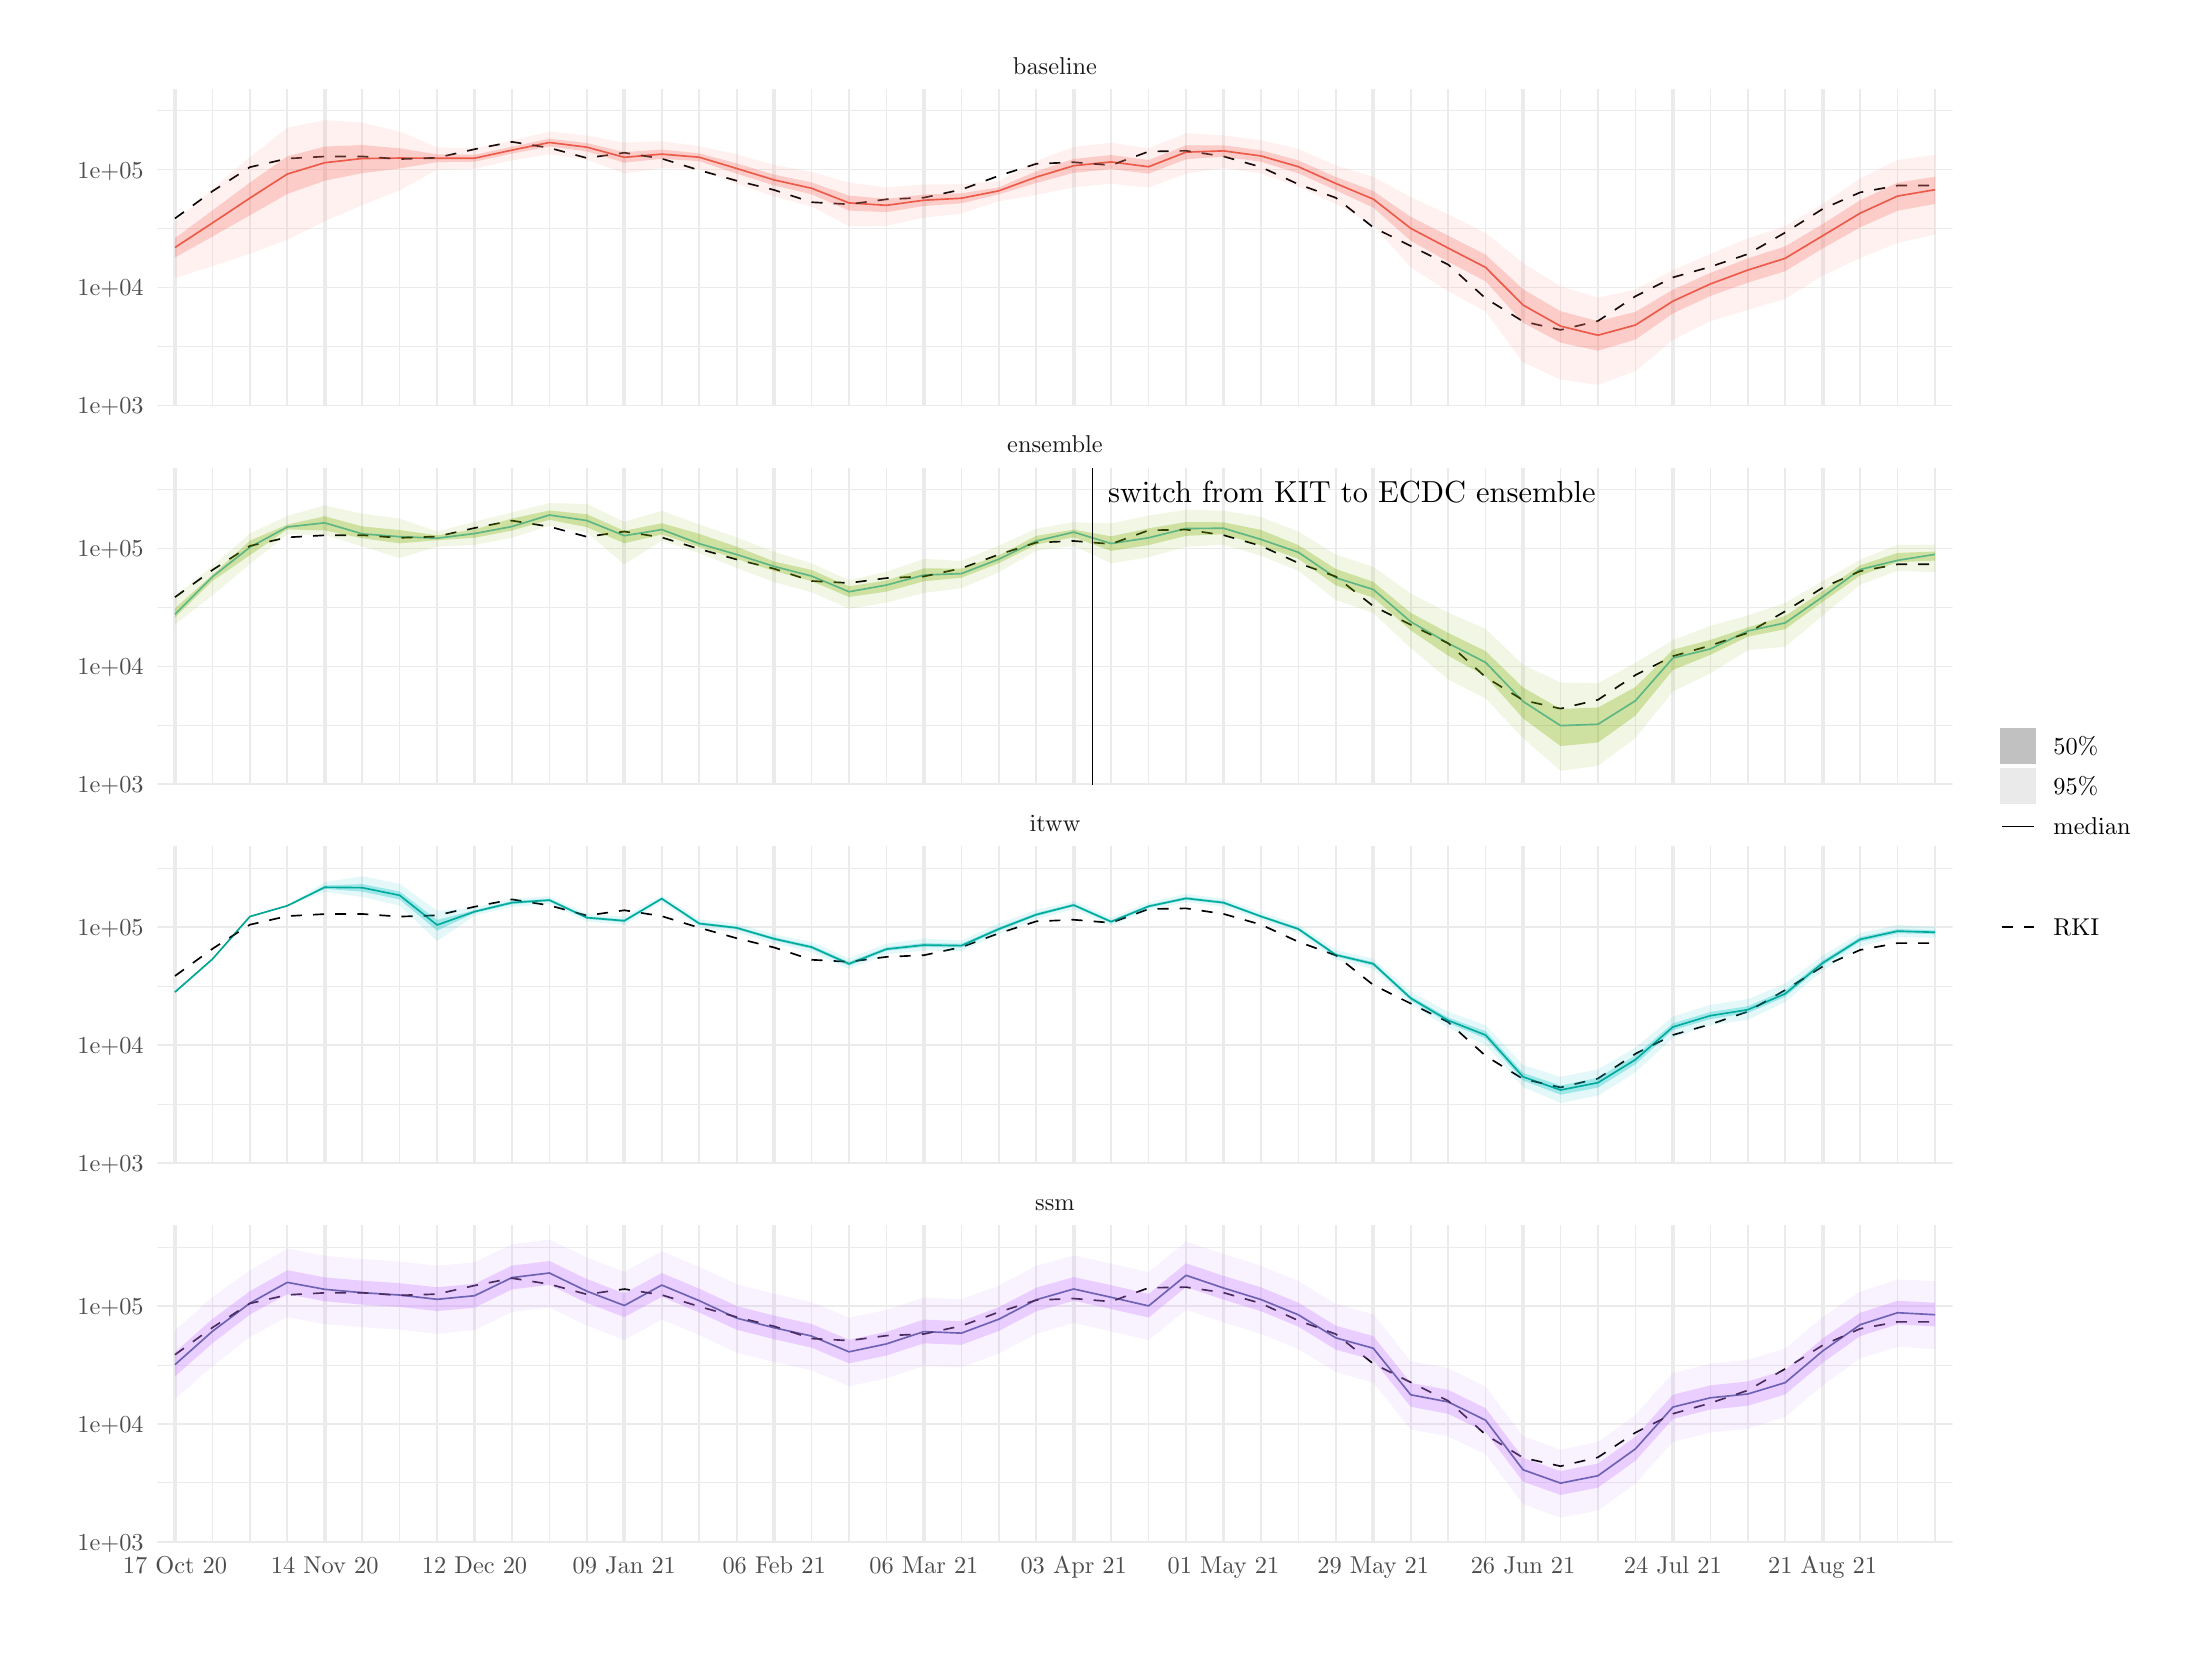
\begin{tikzpicture}[x=1pt,y=1pt]
\definecolor{fillColor}{RGB}{255,255,255}
\path[use as bounding box,fill=fillColor,fill opacity=0.00] (0,0) rectangle (770.88,578.16);
\begin{scope}
\path[clip] ( 46.86,441.29) rectangle (695.57,556.09);
\definecolor{drawColor}{gray}{0.92}

\path[draw=drawColor,line width= 0.3pt,line join=round] ( 46.86,462.93) --
	(695.57,462.93);

\path[draw=drawColor,line width= 0.3pt,line join=round] ( 46.86,505.54) --
	(695.57,505.54);

\path[draw=drawColor,line width= 0.3pt,line join=round] ( 46.86,548.15) --
	(695.57,548.15);

\path[draw=drawColor,line width= 0.6pt,line join=round] ( 66.76,441.29) --
	( 66.76,556.09);

\path[draw=drawColor,line width= 0.6pt,line join=round] ( 80.29,441.29) --
	( 80.29,556.09);

\path[draw=drawColor,line width= 0.6pt,line join=round] ( 93.82,441.29) --
	( 93.82,556.09);

\path[draw=drawColor,line width= 0.6pt,line join=round] (120.88,441.29) --
	(120.88,556.09);

\path[draw=drawColor,line width= 0.6pt,line join=round] (134.41,441.29) --
	(134.41,556.09);

\path[draw=drawColor,line width= 0.6pt,line join=round] (147.94,441.29) --
	(147.94,556.09);

\path[draw=drawColor,line width= 0.6pt,line join=round] (175.01,441.29) --
	(175.01,556.09);

\path[draw=drawColor,line width= 0.6pt,line join=round] (188.54,441.29) --
	(188.54,556.09);

\path[draw=drawColor,line width= 0.6pt,line join=round] (202.07,441.29) --
	(202.07,556.09);

\path[draw=drawColor,line width= 0.6pt,line join=round] (229.13,441.29) --
	(229.13,556.09);

\path[draw=drawColor,line width= 0.6pt,line join=round] (242.67,441.29) --
	(242.67,556.09);

\path[draw=drawColor,line width= 0.6pt,line join=round] (256.20,441.29) --
	(256.20,556.09);

\path[draw=drawColor,line width= 0.6pt,line join=round] (283.26,441.29) --
	(283.26,556.09);

\path[draw=drawColor,line width= 0.6pt,line join=round] (296.79,441.29) --
	(296.79,556.09);

\path[draw=drawColor,line width= 0.6pt,line join=round] (310.32,441.29) --
	(310.32,556.09);

\path[draw=drawColor,line width= 0.6pt,line join=round] (337.39,441.29) --
	(337.39,556.09);

\path[draw=drawColor,line width= 0.6pt,line join=round] (350.92,441.29) --
	(350.92,556.09);

\path[draw=drawColor,line width= 0.6pt,line join=round] (364.45,441.29) --
	(364.45,556.09);

\path[draw=drawColor,line width= 0.6pt,line join=round] (391.51,441.29) --
	(391.51,556.09);

\path[draw=drawColor,line width= 0.6pt,line join=round] (405.04,441.29) --
	(405.04,556.09);

\path[draw=drawColor,line width= 0.6pt,line join=round] (418.58,441.29) --
	(418.58,556.09);

\path[draw=drawColor,line width= 0.6pt,line join=round] (445.64,441.29) --
	(445.64,556.09);

\path[draw=drawColor,line width= 0.6pt,line join=round] (459.17,441.29) --
	(459.17,556.09);

\path[draw=drawColor,line width= 0.6pt,line join=round] (472.70,441.29) --
	(472.70,556.09);

\path[draw=drawColor,line width= 0.6pt,line join=round] (499.76,441.29) --
	(499.76,556.09);

\path[draw=drawColor,line width= 0.6pt,line join=round] (513.30,441.29) --
	(513.30,556.09);

\path[draw=drawColor,line width= 0.6pt,line join=round] (526.83,441.29) --
	(526.83,556.09);

\path[draw=drawColor,line width= 0.6pt,line join=round] (553.89,441.29) --
	(553.89,556.09);

\path[draw=drawColor,line width= 0.6pt,line join=round] (567.42,441.29) --
	(567.42,556.09);

\path[draw=drawColor,line width= 0.6pt,line join=round] (580.95,441.29) --
	(580.95,556.09);

\path[draw=drawColor,line width= 0.6pt,line join=round] (608.02,441.29) --
	(608.02,556.09);

\path[draw=drawColor,line width= 0.6pt,line join=round] (621.55,441.29) --
	(621.55,556.09);

\path[draw=drawColor,line width= 0.6pt,line join=round] (635.08,441.29) --
	(635.08,556.09);

\path[draw=drawColor,line width= 0.6pt,line join=round] (662.14,441.29) --
	(662.14,556.09);

\path[draw=drawColor,line width= 0.6pt,line join=round] (675.67,441.29) --
	(675.67,556.09);

\path[draw=drawColor,line width= 0.6pt,line join=round] (689.21,441.29) --
	(689.21,556.09);

\path[draw=drawColor,line width= 0.6pt,line join=round] ( 46.86,441.63) --
	(695.57,441.63);

\path[draw=drawColor,line width= 0.6pt,line join=round] ( 46.86,484.24) --
	(695.57,484.24);

\path[draw=drawColor,line width= 0.6pt,line join=round] ( 46.86,526.85) --
	(695.57,526.85);

\path[draw=drawColor,line width= 1.4pt,line join=round] ( 53.22,441.29) --
	( 53.22,556.09);

\path[draw=drawColor,line width= 1.4pt,line join=round] (107.35,441.29) --
	(107.35,556.09);

\path[draw=drawColor,line width= 1.4pt,line join=round] (161.48,441.29) --
	(161.48,556.09);

\path[draw=drawColor,line width= 1.4pt,line join=round] (215.60,441.29) --
	(215.60,556.09);

\path[draw=drawColor,line width= 1.4pt,line join=round] (269.73,441.29) --
	(269.73,556.09);

\path[draw=drawColor,line width= 1.4pt,line join=round] (323.85,441.29) --
	(323.85,556.09);

\path[draw=drawColor,line width= 1.4pt,line join=round] (377.98,441.29) --
	(377.98,556.09);

\path[draw=drawColor,line width= 1.4pt,line join=round] (432.11,441.29) --
	(432.11,556.09);

\path[draw=drawColor,line width= 1.4pt,line join=round] (486.23,441.29) --
	(486.23,556.09);

\path[draw=drawColor,line width= 1.4pt,line join=round] (540.36,441.29) --
	(540.36,556.09);

\path[draw=drawColor,line width= 1.4pt,line join=round] (594.49,441.29) --
	(594.49,556.09);

\path[draw=drawColor,line width= 1.4pt,line join=round] (648.61,441.29) --
	(648.61,556.09);
\definecolor{drawColor}{RGB}{230,75,53}

\path[draw=drawColor,line width= 0.6pt,line join=round] ( 53.22,498.71) --
	( 66.76,507.59) --
	( 80.29,516.57) --
	( 93.82,525.26) --
	(107.35,529.36) --
	(120.88,530.87) --
	(134.41,531.04) --
	(147.94,530.98) --
	(161.48,530.98) --
	(175.01,533.91) --
	(188.54,536.67) --
	(202.07,534.97) --
	(215.60,531.31) --
	(229.13,532.46) --
	(242.67,531.34) --
	(256.20,527.27) --
	(269.73,523.13) --
	(283.26,520.12) --
	(296.79,514.83) --
	(310.32,513.96) --
	(323.85,515.80) --
	(337.39,516.52) --
	(350.92,519.20) --
	(364.45,524.16) --
	(377.98,528.27) --
	(391.51,529.65) --
	(405.04,527.90) --
	(418.58,533.18) --
	(432.11,533.63) --
	(445.64,531.80) --
	(459.17,527.91) --
	(472.70,521.85) --
	(486.23,516.20) --
	(499.76,505.64) --
	(513.30,498.50) --
	(526.83,491.51) --
	(540.36,477.92) --
	(553.89,470.30) --
	(567.42,467.01) --
	(580.95,470.70) --
	(594.49,479.32) --
	(608.02,485.54) --
	(621.55,490.56) --
	(635.08,494.82) --
	(648.61,502.96) --
	(662.14,511.10) --
	(675.67,517.30) --
	(689.21,519.60);
\definecolor{drawColor}{RGB}{0,0,0}

\path[draw=drawColor,line width= 0.6pt,dash pattern=on 4pt off 4pt ,line join=round] ( 53.22,509.22) --
	( 66.76,519.04) --
	( 80.29,527.75) --
	( 93.82,530.85) --
	(107.35,531.60) --
	(120.88,531.63) --
	(134.41,530.67) --
	(147.94,531.14) --
	(161.48,534.23) --
	(175.01,536.89) --
	(188.54,534.72) --
	(202.07,531.04) --
	(215.60,532.96) --
	(229.13,530.83) --
	(242.67,526.66) --
	(256.20,522.85) --
	(269.73,519.51) --
	(283.26,515.08) --
	(296.79,514.34) --
	(310.32,516.13) --
	(323.85,516.73) --
	(337.39,519.64) --
	(350.92,524.64) --
	(364.45,528.96) --
	(377.98,529.53) --
	(391.51,528.45) --
	(405.04,533.39) --
	(418.58,533.66) --
	(432.11,531.65) --
	(445.64,527.79) --
	(459.17,521.57) --
	(472.70,516.68) --
	(486.23,505.99) --
	(499.76,499.27) --
	(513.30,492.56) --
	(526.83,480.33) --
	(540.36,472.01) --
	(553.89,468.95) --
	(567.42,472.16) --
	(580.95,481.09) --
	(594.49,487.91) --
	(608.02,491.74) --
	(621.55,496.34) --
	(635.08,504.13) --
	(648.61,512.65) --
	(662.14,518.63) --
	(675.67,521.11) --
	(689.21,521.11);
\definecolor{fillColor}{RGB}{248,118,109}

\path[fill=fillColor,fill opacity=0.30] ( 53.22,502.08) --
	( 66.76,512.12) --
	( 80.29,522.15) --
	( 93.82,531.65) --
	(107.35,535.19) --
	(120.88,535.73) --
	(134.41,534.57) --
	(147.94,532.36) --
	(161.48,532.22) --
	(175.01,535.15) --
	(188.54,538.06) --
	(202.07,536.46) --
	(215.60,533.19) --
	(229.13,534.10) --
	(242.67,532.74) --
	(256.20,529.09) --
	(269.73,525.05) --
	(283.26,522.23) --
	(296.79,517.47) --
	(310.32,516.29) --
	(323.85,517.83) --
	(337.39,518.31) --
	(350.92,520.44) --
	(364.45,526.24) --
	(377.98,530.73) --
	(391.51,532.15) --
	(405.04,530.31) --
	(418.58,535.64) --
	(432.11,535.63) --
	(445.64,533.83) --
	(459.17,530.21) --
	(472.70,524.19) --
	(486.23,519.10) --
	(499.76,509.79) --
	(513.30,503.01) --
	(526.83,496.13) --
	(540.36,483.64) --
	(553.89,475.70) --
	(567.42,472.09) --
	(580.95,475.47) --
	(594.49,483.45) --
	(608.02,489.53) --
	(621.55,494.78) --
	(635.08,499.12) --
	(648.61,507.19) --
	(662.14,515.77) --
	(675.67,522.15) --
	(689.21,524.29) --
	(689.21,514.49) --
	(675.67,512.00) --
	(662.14,506.00) --
	(648.61,498.38) --
	(635.08,490.17) --
	(621.55,486.00) --
	(608.02,481.23) --
	(594.49,474.87) --
	(580.95,465.47) --
	(567.42,461.42) --
	(553.89,464.33) --
	(540.36,471.56) --
	(526.83,486.48) --
	(513.30,493.59) --
	(499.76,501.15) --
	(486.23,513.13) --
	(472.70,519.40) --
	(459.17,525.52) --
	(445.64,529.70) --
	(432.11,531.57) --
	(418.58,530.62) --
	(405.04,525.41) --
	(391.51,527.06) --
	(377.98,525.71) --
	(364.45,522.01) --
	(350.92,517.94) --
	(337.39,514.66) --
	(323.85,513.71) --
	(310.32,511.52) --
	(296.79,512.06) --
	(283.26,517.93) --
	(269.73,521.15) --
	(256.20,525.39) --
	(242.67,529.91) --
	(229.13,530.77) --
	(215.60,529.36) --
	(202.07,533.44) --
	(188.54,535.24) --
	(175.01,532.64) --
	(161.48,529.72) --
	(147.94,529.57) --
	(134.41,527.29) --
	(120.88,525.57) --
	(107.35,522.87) --
	( 93.82,518.06) --
	( 80.29,510.37) --
	( 66.76,502.66) --
	( 53.22,495.12) --
	cycle;

\path[] ( 53.22,502.08) --
	( 66.76,512.12) --
	( 80.29,522.15) --
	( 93.82,531.65) --
	(107.35,535.19) --
	(120.88,535.73) --
	(134.41,534.57) --
	(147.94,532.36) --
	(161.48,532.22) --
	(175.01,535.15) --
	(188.54,538.06) --
	(202.07,536.46) --
	(215.60,533.19) --
	(229.13,534.10) --
	(242.67,532.74) --
	(256.20,529.09) --
	(269.73,525.05) --
	(283.26,522.23) --
	(296.79,517.47) --
	(310.32,516.29) --
	(323.85,517.83) --
	(337.39,518.31) --
	(350.92,520.44) --
	(364.45,526.24) --
	(377.98,530.73) --
	(391.51,532.15) --
	(405.04,530.31) --
	(418.58,535.64) --
	(432.11,535.63) --
	(445.64,533.83) --
	(459.17,530.21) --
	(472.70,524.19) --
	(486.23,519.10) --
	(499.76,509.79) --
	(513.30,503.01) --
	(526.83,496.13) --
	(540.36,483.64) --
	(553.89,475.70) --
	(567.42,472.09) --
	(580.95,475.47) --
	(594.49,483.45) --
	(608.02,489.53) --
	(621.55,494.78) --
	(635.08,499.12) --
	(648.61,507.19) --
	(662.14,515.77) --
	(675.67,522.15) --
	(689.21,524.29);

\path[] (689.21,514.49) --
	(675.67,512.00) --
	(662.14,506.00) --
	(648.61,498.38) --
	(635.08,490.17) --
	(621.55,486.00) --
	(608.02,481.23) --
	(594.49,474.87) --
	(580.95,465.47) --
	(567.42,461.42) --
	(553.89,464.33) --
	(540.36,471.56) --
	(526.83,486.48) --
	(513.30,493.59) --
	(499.76,501.15) --
	(486.23,513.13) --
	(472.70,519.40) --
	(459.17,525.52) --
	(445.64,529.70) --
	(432.11,531.57) --
	(418.58,530.62) --
	(405.04,525.41) --
	(391.51,527.06) --
	(377.98,525.71) --
	(364.45,522.01) --
	(350.92,517.94) --
	(337.39,514.66) --
	(323.85,513.71) --
	(310.32,511.52) --
	(296.79,512.06) --
	(283.26,517.93) --
	(269.73,521.15) --
	(256.20,525.39) --
	(242.67,529.91) --
	(229.13,530.77) --
	(215.60,529.36) --
	(202.07,533.44) --
	(188.54,535.24) --
	(175.01,532.64) --
	(161.48,529.72) --
	(147.94,529.57) --
	(134.41,527.29) --
	(120.88,525.57) --
	(107.35,522.87) --
	( 93.82,518.06) --
	( 80.29,510.37) --
	( 66.76,502.66) --
	( 53.22,495.12);
\definecolor{fillColor}{RGB}{248,118,109}

\path[fill=fillColor,fill opacity=0.10] ( 53.22,507.97) --
	( 66.76,519.81) --
	( 80.29,531.40) --
	( 93.82,542.01) --
	(107.35,544.75) --
	(120.88,543.87) --
	(134.41,540.68) --
	(147.94,534.89) --
	(161.48,534.50) --
	(175.01,537.43) --
	(188.54,540.61) --
	(202.07,539.18) --
	(215.60,536.61) --
	(229.13,537.10) --
	(242.67,535.31) --
	(256.20,532.39) --
	(269.73,528.54) --
	(283.26,526.04) --
	(296.79,522.16) --
	(310.32,520.47) --
	(323.85,521.48) --
	(337.39,521.58) --
	(350.92,522.72) --
	(364.45,530.00) --
	(377.98,535.09) --
	(391.51,536.56) --
	(405.04,534.59) --
	(418.58,539.99) --
	(432.11,539.23) --
	(445.64,537.49) --
	(459.17,534.33) --
	(472.70,528.41) --
	(486.23,524.24) --
	(499.76,516.91) --
	(513.30,510.67) --
	(526.83,503.97) --
	(540.36,493.07) --
	(553.89,484.68) --
	(567.42,480.61) --
	(580.95,483.54) --
	(594.49,490.53) --
	(608.02,496.41) --
	(621.55,502.00) --
	(635.08,506.46) --
	(648.61,514.43) --
	(662.14,523.68) --
	(675.67,530.31) --
	(689.21,532.21) --
	(689.21,503.35) --
	(675.67,500.39) --
	(662.14,494.88) --
	(648.61,488.54) --
	(635.08,480.14) --
	(621.55,476.19) --
	(608.02,472.04) --
	(594.49,465.31) --
	(580.95,454.05) --
	(567.42,449.08) --
	(553.89,451.00) --
	(540.36,457.23) --
	(526.83,475.51) --
	(513.30,482.95) --
	(499.76,491.52) --
	(486.23,506.80) --
	(472.70,514.43) --
	(459.17,520.66) --
	(445.64,525.48) --
	(432.11,527.42) --
	(418.58,525.41) --
	(405.04,520.33) --
	(391.51,521.76) --
	(377.98,520.49) --
	(364.45,517.65) --
	(350.92,515.44) --
	(337.39,510.95) --
	(323.85,509.48) --
	(310.32,506.58) --
	(296.79,506.39) --
	(283.26,513.50) --
	(269.73,517.16) --
	(256.20,521.64) --
	(242.67,527.08) --
	(229.13,527.40) --
	(215.60,525.45) --
	(202.07,530.42) --
	(188.54,532.42) --
	(175.01,530.15) --
	(161.48,527.23) --
	(147.94,526.79) --
	(134.41,519.38) --
	(120.88,513.96) --
	(107.35,508.22) --
	( 93.82,501.52) --
	( 80.29,496.47) --
	( 66.76,491.97) --
	( 53.22,487.61) --
	cycle;

\path[] ( 53.22,507.97) --
	( 66.76,519.81) --
	( 80.29,531.40) --
	( 93.82,542.01) --
	(107.35,544.75) --
	(120.88,543.87) --
	(134.41,540.68) --
	(147.94,534.89) --
	(161.48,534.50) --
	(175.01,537.43) --
	(188.54,540.61) --
	(202.07,539.18) --
	(215.60,536.61) --
	(229.13,537.10) --
	(242.67,535.31) --
	(256.20,532.39) --
	(269.73,528.54) --
	(283.26,526.04) --
	(296.79,522.16) --
	(310.32,520.47) --
	(323.85,521.48) --
	(337.39,521.58) --
	(350.92,522.72) --
	(364.45,530.00) --
	(377.98,535.09) --
	(391.51,536.56) --
	(405.04,534.59) --
	(418.58,539.99) --
	(432.11,539.23) --
	(445.64,537.49) --
	(459.17,534.33) --
	(472.70,528.41) --
	(486.23,524.24) --
	(499.76,516.91) --
	(513.30,510.67) --
	(526.83,503.97) --
	(540.36,493.07) --
	(553.89,484.68) --
	(567.42,480.61) --
	(580.95,483.54) --
	(594.49,490.53) --
	(608.02,496.41) --
	(621.55,502.00) --
	(635.08,506.46) --
	(648.61,514.43) --
	(662.14,523.68) --
	(675.67,530.31) --
	(689.21,532.21);

\path[] (689.21,503.35) --
	(675.67,500.39) --
	(662.14,494.88) --
	(648.61,488.54) --
	(635.08,480.14) --
	(621.55,476.19) --
	(608.02,472.04) --
	(594.49,465.31) --
	(580.95,454.05) --
	(567.42,449.08) --
	(553.89,451.00) --
	(540.36,457.23) --
	(526.83,475.51) --
	(513.30,482.95) --
	(499.76,491.52) --
	(486.23,506.80) --
	(472.70,514.43) --
	(459.17,520.66) --
	(445.64,525.48) --
	(432.11,527.42) --
	(418.58,525.41) --
	(405.04,520.33) --
	(391.51,521.76) --
	(377.98,520.49) --
	(364.45,517.65) --
	(350.92,515.44) --
	(337.39,510.95) --
	(323.85,509.48) --
	(310.32,506.58) --
	(296.79,506.39) --
	(283.26,513.50) --
	(269.73,517.16) --
	(256.20,521.64) --
	(242.67,527.08) --
	(229.13,527.40) --
	(215.60,525.45) --
	(202.07,530.42) --
	(188.54,532.42) --
	(175.01,530.15) --
	(161.48,527.23) --
	(147.94,526.79) --
	(134.41,519.38) --
	(120.88,513.96) --
	(107.35,508.22) --
	( 93.82,501.52) --
	( 80.29,496.47) --
	( 66.76,491.97) --
	( 53.22,487.61);
\end{scope}
\begin{scope}
\path[clip] ( 46.86,304.42) rectangle (695.57,419.22);
\definecolor{drawColor}{gray}{0.92}

\path[draw=drawColor,line width= 0.3pt,line join=round] ( 46.86,326.06) --
	(695.57,326.06);

\path[draw=drawColor,line width= 0.3pt,line join=round] ( 46.86,368.67) --
	(695.57,368.67);

\path[draw=drawColor,line width= 0.3pt,line join=round] ( 46.86,411.28) --
	(695.57,411.28);

\path[draw=drawColor,line width= 0.6pt,line join=round] ( 66.76,304.42) --
	( 66.76,419.22);

\path[draw=drawColor,line width= 0.6pt,line join=round] ( 80.29,304.42) --
	( 80.29,419.22);

\path[draw=drawColor,line width= 0.6pt,line join=round] ( 93.82,304.42) --
	( 93.82,419.22);

\path[draw=drawColor,line width= 0.6pt,line join=round] (120.88,304.42) --
	(120.88,419.22);

\path[draw=drawColor,line width= 0.6pt,line join=round] (134.41,304.42) --
	(134.41,419.22);

\path[draw=drawColor,line width= 0.6pt,line join=round] (147.94,304.42) --
	(147.94,419.22);

\path[draw=drawColor,line width= 0.6pt,line join=round] (175.01,304.42) --
	(175.01,419.22);

\path[draw=drawColor,line width= 0.6pt,line join=round] (188.54,304.42) --
	(188.54,419.22);

\path[draw=drawColor,line width= 0.6pt,line join=round] (202.07,304.42) --
	(202.07,419.22);

\path[draw=drawColor,line width= 0.6pt,line join=round] (229.13,304.42) --
	(229.13,419.22);

\path[draw=drawColor,line width= 0.6pt,line join=round] (242.67,304.42) --
	(242.67,419.22);

\path[draw=drawColor,line width= 0.6pt,line join=round] (256.20,304.42) --
	(256.20,419.22);

\path[draw=drawColor,line width= 0.6pt,line join=round] (283.26,304.42) --
	(283.26,419.22);

\path[draw=drawColor,line width= 0.6pt,line join=round] (296.79,304.42) --
	(296.79,419.22);

\path[draw=drawColor,line width= 0.6pt,line join=round] (310.32,304.42) --
	(310.32,419.22);

\path[draw=drawColor,line width= 0.6pt,line join=round] (337.39,304.42) --
	(337.39,419.22);

\path[draw=drawColor,line width= 0.6pt,line join=round] (350.92,304.42) --
	(350.92,419.22);

\path[draw=drawColor,line width= 0.6pt,line join=round] (364.45,304.42) --
	(364.45,419.22);

\path[draw=drawColor,line width= 0.6pt,line join=round] (391.51,304.42) --
	(391.51,419.22);

\path[draw=drawColor,line width= 0.6pt,line join=round] (405.04,304.42) --
	(405.04,419.22);

\path[draw=drawColor,line width= 0.6pt,line join=round] (418.58,304.42) --
	(418.58,419.22);

\path[draw=drawColor,line width= 0.6pt,line join=round] (445.64,304.42) --
	(445.64,419.22);

\path[draw=drawColor,line width= 0.6pt,line join=round] (459.17,304.42) --
	(459.17,419.22);

\path[draw=drawColor,line width= 0.6pt,line join=round] (472.70,304.42) --
	(472.70,419.22);

\path[draw=drawColor,line width= 0.6pt,line join=round] (499.76,304.42) --
	(499.76,419.22);

\path[draw=drawColor,line width= 0.6pt,line join=round] (513.30,304.42) --
	(513.30,419.22);

\path[draw=drawColor,line width= 0.6pt,line join=round] (526.83,304.42) --
	(526.83,419.22);

\path[draw=drawColor,line width= 0.6pt,line join=round] (553.89,304.42) --
	(553.89,419.22);

\path[draw=drawColor,line width= 0.6pt,line join=round] (567.42,304.42) --
	(567.42,419.22);

\path[draw=drawColor,line width= 0.6pt,line join=round] (580.95,304.42) --
	(580.95,419.22);

\path[draw=drawColor,line width= 0.6pt,line join=round] (608.02,304.42) --
	(608.02,419.22);

\path[draw=drawColor,line width= 0.6pt,line join=round] (621.55,304.42) --
	(621.55,419.22);

\path[draw=drawColor,line width= 0.6pt,line join=round] (635.08,304.42) --
	(635.08,419.22);

\path[draw=drawColor,line width= 0.6pt,line join=round] (662.14,304.42) --
	(662.14,419.22);

\path[draw=drawColor,line width= 0.6pt,line join=round] (675.67,304.42) --
	(675.67,419.22);

\path[draw=drawColor,line width= 0.6pt,line join=round] (689.21,304.42) --
	(689.21,419.22);

\path[draw=drawColor,line width= 0.6pt,line join=round] ( 46.86,304.76) --
	(695.57,304.76);

\path[draw=drawColor,line width= 0.6pt,line join=round] ( 46.86,347.37) --
	(695.57,347.37);

\path[draw=drawColor,line width= 0.6pt,line join=round] ( 46.86,389.98) --
	(695.57,389.98);

\path[draw=drawColor,line width= 1.4pt,line join=round] ( 53.22,304.42) --
	( 53.22,419.22);

\path[draw=drawColor,line width= 1.4pt,line join=round] (107.35,304.42) --
	(107.35,419.22);

\path[draw=drawColor,line width= 1.4pt,line join=round] (161.48,304.42) --
	(161.48,419.22);

\path[draw=drawColor,line width= 1.4pt,line join=round] (215.60,304.42) --
	(215.60,419.22);

\path[draw=drawColor,line width= 1.4pt,line join=round] (269.73,304.42) --
	(269.73,419.22);

\path[draw=drawColor,line width= 1.4pt,line join=round] (323.85,304.42) --
	(323.85,419.22);

\path[draw=drawColor,line width= 1.4pt,line join=round] (377.98,304.42) --
	(377.98,419.22);

\path[draw=drawColor,line width= 1.4pt,line join=round] (432.11,304.42) --
	(432.11,419.22);

\path[draw=drawColor,line width= 1.4pt,line join=round] (486.23,304.42) --
	(486.23,419.22);

\path[draw=drawColor,line width= 1.4pt,line join=round] (540.36,304.42) --
	(540.36,419.22);

\path[draw=drawColor,line width= 1.4pt,line join=round] (594.49,304.42) --
	(594.49,419.22);

\path[draw=drawColor,line width= 1.4pt,line join=round] (648.61,304.42) --
	(648.61,419.22);
\definecolor{drawColor}{RGB}{77,187,213}

\path[draw=drawColor,line width= 0.6pt,line join=round] ( 53.22,366.17) --
	( 66.76,379.73) --
	( 80.29,390.40) --
	( 93.82,397.73) --
	(107.35,399.23) --
	(120.88,395.25) --
	(134.41,394.21) --
	(147.94,393.68) --
	(161.48,395.35) --
	(175.01,397.89) --
	(188.54,402.05) --
	(202.07,400.05) --
	(215.60,394.58) --
	(229.13,396.79) --
	(242.67,391.70) --
	(256.20,387.77) --
	(269.73,383.48) --
	(283.26,380.00) --
	(296.79,374.33) --
	(310.32,376.75) --
	(323.85,380.37) --
	(337.39,380.88) --
	(350.92,386.09) --
	(364.45,392.66) --
	(377.98,395.87) --
	(391.51,391.74) --
	(405.04,393.82) --
	(418.58,397.18) --
	(432.11,397.27) --
	(445.64,393.24) --
	(459.17,388.57) --
	(472.70,379.37) --
	(486.23,375.15) --
	(499.76,363.49) --
	(513.30,355.72) --
	(526.83,348.77) --
	(540.36,334.70) --
	(553.89,325.95) --
	(567.42,326.44) --
	(580.95,334.94) --
	(594.49,350.36) --
	(608.02,353.66) --
	(621.55,360.15) --
	(635.08,363.08) --
	(648.61,372.48) --
	(662.14,382.36) --
	(675.67,385.67) --
	(689.21,387.83);
\definecolor{drawColor}{RGB}{0,0,0}

\path[draw=drawColor,line width= 0.6pt,dash pattern=on 4pt off 4pt ,line join=round] ( 53.22,372.36) --
	( 66.76,382.17) --
	( 80.29,390.88) --
	( 93.82,393.98) --
	(107.35,394.73) --
	(120.88,394.76) --
	(134.41,393.81) --
	(147.94,394.27) --
	(161.48,397.36) --
	(175.01,400.02) --
	(188.54,397.86) --
	(202.07,394.18) --
	(215.60,396.09) --
	(229.13,393.96) --
	(242.67,389.79) --
	(256.20,385.99) --
	(269.73,382.65) --
	(283.26,378.21) --
	(296.79,377.48) --
	(310.32,379.26) --
	(323.85,379.86) --
	(337.39,382.77) --
	(350.92,387.77) --
	(364.45,392.09) --
	(377.98,392.67) --
	(391.51,391.58) --
	(405.04,396.52) --
	(418.58,396.79) --
	(432.11,394.78) --
	(445.64,390.92) --
	(459.17,384.70) --
	(472.70,379.81) --
	(486.23,369.12) --
	(499.76,362.40) --
	(513.30,355.69) --
	(526.83,343.47) --
	(540.36,335.14) --
	(553.89,332.08) --
	(567.42,335.29) --
	(580.95,344.22) --
	(594.49,351.04) --
	(608.02,354.88) --
	(621.55,359.47) --
	(635.08,367.26) --
	(648.61,375.78) --
	(662.14,381.76) --
	(675.67,384.24) --
	(689.21,384.24);
\definecolor{fillColor}{RGB}{124,174,0}

\path[fill=fillColor,fill opacity=0.30] ( 53.22,368.35) --
	( 66.76,380.42) --
	( 80.29,392.78) --
	( 93.82,398.58) --
	(107.35,401.61) --
	(120.88,397.94) --
	(134.41,396.62) --
	(147.94,394.71) --
	(161.48,396.86) --
	(175.01,400.78) --
	(188.54,403.69) --
	(202.07,402.33) --
	(215.60,396.35) --
	(229.13,399.10) --
	(242.67,395.27) --
	(256.20,390.59) --
	(269.73,385.25) --
	(283.26,382.20) --
	(296.79,376.28) --
	(310.32,378.43) --
	(323.85,382.76) --
	(337.39,382.69) --
	(350.92,387.48) --
	(364.45,394.53) --
	(377.98,396.78) --
	(391.51,394.36) --
	(405.04,397.22) --
	(418.58,399.52) --
	(432.11,399.42) --
	(445.64,396.66) --
	(459.17,391.18) --
	(472.70,382.54) --
	(486.23,377.92) --
	(499.76,366.73) --
	(513.30,359.45) --
	(526.83,352.87) --
	(540.36,339.71) --
	(553.89,331.98) --
	(567.42,332.50) --
	(580.95,339.89) --
	(594.49,353.37) --
	(608.02,356.91) --
	(621.55,361.42) --
	(635.08,365.59) --
	(648.61,374.57) --
	(662.14,383.86) --
	(675.67,388.35) --
	(689.21,388.84) --
	(689.21,385.59) --
	(675.67,384.98) --
	(662.14,380.18) --
	(648.61,370.66) --
	(635.08,360.81) --
	(621.55,358.09) --
	(608.02,351.52) --
	(594.49,346.03) --
	(580.95,329.56) --
	(567.42,319.85) --
	(553.89,318.57) --
	(540.36,328.55) --
	(526.83,343.77) --
	(513.30,351.22) --
	(499.76,360.40) --
	(486.23,372.19) --
	(472.70,376.62) --
	(459.17,386.21) --
	(445.64,391.05) --
	(432.11,395.12) --
	(418.58,394.52) --
	(405.04,391.17) --
	(391.51,389.08) --
	(377.98,394.01) --
	(364.45,391.40) --
	(350.92,384.62) --
	(337.39,379.40) --
	(323.85,378.12) --
	(310.32,374.37) --
	(296.79,372.43) --
	(283.26,378.15) --
	(269.73,381.82) --
	(256.20,386.19) --
	(242.67,390.47) --
	(229.13,395.03) --
	(215.60,391.84) --
	(202.07,397.63) --
	(188.54,400.32) --
	(175.01,396.45) --
	(161.48,393.82) --
	(147.94,392.95) --
	(134.41,391.80) --
	(120.88,393.67) --
	(107.35,396.46) --
	( 93.82,396.87) --
	( 80.29,387.52) --
	( 66.76,378.21) --
	( 53.22,365.00) --
	cycle;

\path[] ( 53.22,368.35) --
	( 66.76,380.42) --
	( 80.29,392.78) --
	( 93.82,398.58) --
	(107.35,401.61) --
	(120.88,397.94) --
	(134.41,396.62) --
	(147.94,394.71) --
	(161.48,396.86) --
	(175.01,400.78) --
	(188.54,403.69) --
	(202.07,402.33) --
	(215.60,396.35) --
	(229.13,399.10) --
	(242.67,395.27) --
	(256.20,390.59) --
	(269.73,385.25) --
	(283.26,382.20) --
	(296.79,376.28) --
	(310.32,378.43) --
	(323.85,382.76) --
	(337.39,382.69) --
	(350.92,387.48) --
	(364.45,394.53) --
	(377.98,396.78) --
	(391.51,394.36) --
	(405.04,397.22) --
	(418.58,399.52) --
	(432.11,399.42) --
	(445.64,396.66) --
	(459.17,391.18) --
	(472.70,382.54) --
	(486.23,377.92) --
	(499.76,366.73) --
	(513.30,359.45) --
	(526.83,352.87) --
	(540.36,339.71) --
	(553.89,331.98) --
	(567.42,332.50) --
	(580.95,339.89) --
	(594.49,353.37) --
	(608.02,356.91) --
	(621.55,361.42) --
	(635.08,365.59) --
	(648.61,374.57) --
	(662.14,383.86) --
	(675.67,388.35) --
	(689.21,388.84);

\path[] (689.21,385.59) --
	(675.67,384.98) --
	(662.14,380.18) --
	(648.61,370.66) --
	(635.08,360.81) --
	(621.55,358.09) --
	(608.02,351.52) --
	(594.49,346.03) --
	(580.95,329.56) --
	(567.42,319.85) --
	(553.89,318.57) --
	(540.36,328.55) --
	(526.83,343.77) --
	(513.30,351.22) --
	(499.76,360.40) --
	(486.23,372.19) --
	(472.70,376.62) --
	(459.17,386.21) --
	(445.64,391.05) --
	(432.11,395.12) --
	(418.58,394.52) --
	(405.04,391.17) --
	(391.51,389.08) --
	(377.98,394.01) --
	(364.45,391.40) --
	(350.92,384.62) --
	(337.39,379.40) --
	(323.85,378.12) --
	(310.32,374.37) --
	(296.79,372.43) --
	(283.26,378.15) --
	(269.73,381.82) --
	(256.20,386.19) --
	(242.67,390.47) --
	(229.13,395.03) --
	(215.60,391.84) --
	(202.07,397.63) --
	(188.54,400.32) --
	(175.01,396.45) --
	(161.48,393.82) --
	(147.94,392.95) --
	(134.41,391.80) --
	(120.88,393.67) --
	(107.35,396.46) --
	( 93.82,396.87) --
	( 80.29,387.52) --
	( 66.76,378.21) --
	( 53.22,365.00);
\definecolor{fillColor}{RGB}{124,174,0}

\path[fill=fillColor,fill opacity=0.10] ( 53.22,372.77) --
	( 66.76,383.54) --
	( 80.29,395.38) --
	( 93.82,401.75) --
	(107.35,405.54) --
	(120.88,402.53) --
	(134.41,400.78) --
	(147.94,396.06) --
	(161.48,399.64) --
	(175.01,402.96) --
	(188.54,406.39) --
	(202.07,406.01) --
	(215.60,399.60) --
	(229.13,403.58) --
	(242.67,398.63) --
	(256.20,393.99) --
	(269.73,388.76) --
	(283.26,384.56) --
	(296.79,378.52) --
	(310.32,381.55) --
	(323.85,386.20) --
	(337.39,385.44) --
	(350.92,390.99) --
	(364.45,397.12) --
	(377.98,399.44) --
	(391.51,399.00) --
	(405.04,401.85) --
	(418.58,403.94) --
	(432.11,403.63) --
	(445.64,401.35) --
	(459.17,396.06) --
	(472.70,387.76) --
	(486.23,383.34) --
	(499.76,373.67) --
	(513.30,366.77) --
	(526.83,360.91) --
	(540.36,347.93) --
	(553.89,341.56) --
	(567.42,341.21) --
	(580.95,348.65) --
	(594.49,356.85) --
	(608.02,362.01) --
	(621.55,365.76) --
	(635.08,370.30) --
	(648.61,378.14) --
	(662.14,385.86) --
	(675.67,391.38) --
	(689.21,391.31) --
	(689.21,381.42) --
	(675.67,381.89) --
	(662.14,376.90) --
	(648.61,365.74) --
	(635.08,354.42) --
	(621.55,353.22) --
	(608.02,344.78) --
	(594.49,338.30) --
	(580.95,321.48) --
	(567.42,311.39) --
	(553.89,309.64) --
	(540.36,321.44) --
	(526.83,335.78) --
	(513.30,342.64) --
	(499.76,353.97) --
	(486.23,366.66) --
	(472.70,371.33) --
	(459.17,381.91) --
	(445.64,387.33) --
	(432.11,391.32) --
	(418.58,390.58) --
	(405.04,386.77) --
	(391.51,384.62) --
	(377.98,390.88) --
	(364.45,389.17) --
	(350.92,381.34) --
	(337.39,375.57) --
	(323.85,373.91) --
	(310.32,370.38) --
	(296.79,368.15) --
	(283.26,374.13) --
	(269.73,377.80) --
	(256.20,382.90) --
	(242.67,388.29) --
	(229.13,392.80) --
	(215.60,384.21) --
	(202.07,395.73) --
	(188.54,398.14) --
	(175.01,393.84) --
	(161.48,391.23) --
	(147.94,390.64) --
	(134.41,386.43) --
	(120.88,390.71) --
	(107.35,394.83) --
	( 93.82,395.07) --
	( 80.29,384.32) --
	( 66.76,373.03) --
	( 53.22,362.43) --
	cycle;

\path[] ( 53.22,372.77) --
	( 66.76,383.54) --
	( 80.29,395.38) --
	( 93.82,401.75) --
	(107.35,405.54) --
	(120.88,402.53) --
	(134.41,400.78) --
	(147.94,396.06) --
	(161.48,399.64) --
	(175.01,402.96) --
	(188.54,406.39) --
	(202.07,406.01) --
	(215.60,399.60) --
	(229.13,403.58) --
	(242.67,398.63) --
	(256.20,393.99) --
	(269.73,388.76) --
	(283.26,384.56) --
	(296.79,378.52) --
	(310.32,381.55) --
	(323.85,386.20) --
	(337.39,385.44) --
	(350.92,390.99) --
	(364.45,397.12) --
	(377.98,399.44) --
	(391.51,399.00) --
	(405.04,401.85) --
	(418.58,403.94) --
	(432.11,403.63) --
	(445.64,401.35) --
	(459.17,396.06) --
	(472.70,387.76) --
	(486.23,383.34) --
	(499.76,373.67) --
	(513.30,366.77) --
	(526.83,360.91) --
	(540.36,347.93) --
	(553.89,341.56) --
	(567.42,341.21) --
	(580.95,348.65) --
	(594.49,356.85) --
	(608.02,362.01) --
	(621.55,365.76) --
	(635.08,370.30) --
	(648.61,378.14) --
	(662.14,385.86) --
	(675.67,391.38) --
	(689.21,391.31);

\path[] (689.21,381.42) --
	(675.67,381.89) --
	(662.14,376.90) --
	(648.61,365.74) --
	(635.08,354.42) --
	(621.55,353.22) --
	(608.02,344.78) --
	(594.49,338.30) --
	(580.95,321.48) --
	(567.42,311.39) --
	(553.89,309.64) --
	(540.36,321.44) --
	(526.83,335.78) --
	(513.30,342.64) --
	(499.76,353.97) --
	(486.23,366.66) --
	(472.70,371.33) --
	(459.17,381.91) --
	(445.64,387.33) --
	(432.11,391.32) --
	(418.58,390.58) --
	(405.04,386.77) --
	(391.51,384.62) --
	(377.98,390.88) --
	(364.45,389.17) --
	(350.92,381.34) --
	(337.39,375.57) --
	(323.85,373.91) --
	(310.32,370.38) --
	(296.79,368.15) --
	(283.26,374.13) --
	(269.73,377.80) --
	(256.20,382.90) --
	(242.67,388.29) --
	(229.13,392.80) --
	(215.60,384.21) --
	(202.07,395.73) --
	(188.54,398.14) --
	(175.01,393.84) --
	(161.48,391.23) --
	(147.94,390.64) --
	(134.41,386.43) --
	(120.88,390.71) --
	(107.35,394.83) --
	( 93.82,395.07) --
	( 80.29,384.32) --
	( 66.76,373.03) --
	( 53.22,362.43);

\path[draw=drawColor,line width= 0.6pt,line join=round] (384.75,304.42) -- (384.75,419.22);

\node[text=drawColor,anchor=base,inner sep=0pt, outer sep=0pt, scale=  1.10] at (478.50,406.51) {switch from KIT to ECDC ensemble};
\end{scope}
\begin{scope}
\path[clip] ( 46.86,167.55) rectangle (695.57,282.35);
\definecolor{drawColor}{gray}{0.92}

\path[draw=drawColor,line width= 0.3pt,line join=round] ( 46.86,189.19) --
	(695.57,189.19);

\path[draw=drawColor,line width= 0.3pt,line join=round] ( 46.86,231.80) --
	(695.57,231.80);

\path[draw=drawColor,line width= 0.3pt,line join=round] ( 46.86,274.41) --
	(695.57,274.41);

\path[draw=drawColor,line width= 0.6pt,line join=round] ( 66.76,167.55) --
	( 66.76,282.35);

\path[draw=drawColor,line width= 0.6pt,line join=round] ( 80.29,167.55) --
	( 80.29,282.35);

\path[draw=drawColor,line width= 0.6pt,line join=round] ( 93.82,167.55) --
	( 93.82,282.35);

\path[draw=drawColor,line width= 0.6pt,line join=round] (120.88,167.55) --
	(120.88,282.35);

\path[draw=drawColor,line width= 0.6pt,line join=round] (134.41,167.55) --
	(134.41,282.35);

\path[draw=drawColor,line width= 0.6pt,line join=round] (147.94,167.55) --
	(147.94,282.35);

\path[draw=drawColor,line width= 0.6pt,line join=round] (175.01,167.55) --
	(175.01,282.35);

\path[draw=drawColor,line width= 0.6pt,line join=round] (188.54,167.55) --
	(188.54,282.35);

\path[draw=drawColor,line width= 0.6pt,line join=round] (202.07,167.55) --
	(202.07,282.35);

\path[draw=drawColor,line width= 0.6pt,line join=round] (229.13,167.55) --
	(229.13,282.35);

\path[draw=drawColor,line width= 0.6pt,line join=round] (242.67,167.55) --
	(242.67,282.35);

\path[draw=drawColor,line width= 0.6pt,line join=round] (256.20,167.55) --
	(256.20,282.35);

\path[draw=drawColor,line width= 0.6pt,line join=round] (283.26,167.55) --
	(283.26,282.35);

\path[draw=drawColor,line width= 0.6pt,line join=round] (296.79,167.55) --
	(296.79,282.35);

\path[draw=drawColor,line width= 0.6pt,line join=round] (310.32,167.55) --
	(310.32,282.35);

\path[draw=drawColor,line width= 0.6pt,line join=round] (337.39,167.55) --
	(337.39,282.35);

\path[draw=drawColor,line width= 0.6pt,line join=round] (350.92,167.55) --
	(350.92,282.35);

\path[draw=drawColor,line width= 0.6pt,line join=round] (364.45,167.55) --
	(364.45,282.35);

\path[draw=drawColor,line width= 0.6pt,line join=round] (391.51,167.55) --
	(391.51,282.35);

\path[draw=drawColor,line width= 0.6pt,line join=round] (405.04,167.55) --
	(405.04,282.35);

\path[draw=drawColor,line width= 0.6pt,line join=round] (418.58,167.55) --
	(418.58,282.35);

\path[draw=drawColor,line width= 0.6pt,line join=round] (445.64,167.55) --
	(445.64,282.35);

\path[draw=drawColor,line width= 0.6pt,line join=round] (459.17,167.55) --
	(459.17,282.35);

\path[draw=drawColor,line width= 0.6pt,line join=round] (472.70,167.55) --
	(472.70,282.35);

\path[draw=drawColor,line width= 0.6pt,line join=round] (499.76,167.55) --
	(499.76,282.35);

\path[draw=drawColor,line width= 0.6pt,line join=round] (513.30,167.55) --
	(513.30,282.35);

\path[draw=drawColor,line width= 0.6pt,line join=round] (526.83,167.55) --
	(526.83,282.35);

\path[draw=drawColor,line width= 0.6pt,line join=round] (553.89,167.55) --
	(553.89,282.35);

\path[draw=drawColor,line width= 0.6pt,line join=round] (567.42,167.55) --
	(567.42,282.35);

\path[draw=drawColor,line width= 0.6pt,line join=round] (580.95,167.55) --
	(580.95,282.35);

\path[draw=drawColor,line width= 0.6pt,line join=round] (608.02,167.55) --
	(608.02,282.35);

\path[draw=drawColor,line width= 0.6pt,line join=round] (621.55,167.55) --
	(621.55,282.35);

\path[draw=drawColor,line width= 0.6pt,line join=round] (635.08,167.55) --
	(635.08,282.35);

\path[draw=drawColor,line width= 0.6pt,line join=round] (662.14,167.55) --
	(662.14,282.35);

\path[draw=drawColor,line width= 0.6pt,line join=round] (675.67,167.55) --
	(675.67,282.35);

\path[draw=drawColor,line width= 0.6pt,line join=round] (689.21,167.55) --
	(689.21,282.35);

\path[draw=drawColor,line width= 0.6pt,line join=round] ( 46.86,167.89) --
	(695.57,167.89);

\path[draw=drawColor,line width= 0.6pt,line join=round] ( 46.86,210.50) --
	(695.57,210.50);

\path[draw=drawColor,line width= 0.6pt,line join=round] ( 46.86,253.11) --
	(695.57,253.11);

\path[draw=drawColor,line width= 1.4pt,line join=round] ( 53.22,167.55) --
	( 53.22,282.35);

\path[draw=drawColor,line width= 1.4pt,line join=round] (107.35,167.55) --
	(107.35,282.35);

\path[draw=drawColor,line width= 1.4pt,line join=round] (161.48,167.55) --
	(161.48,282.35);

\path[draw=drawColor,line width= 1.4pt,line join=round] (215.60,167.55) --
	(215.60,282.35);

\path[draw=drawColor,line width= 1.4pt,line join=round] (269.73,167.55) --
	(269.73,282.35);

\path[draw=drawColor,line width= 1.4pt,line join=round] (323.85,167.55) --
	(323.85,282.35);

\path[draw=drawColor,line width= 1.4pt,line join=round] (377.98,167.55) --
	(377.98,282.35);

\path[draw=drawColor,line width= 1.4pt,line join=round] (432.11,167.55) --
	(432.11,282.35);

\path[draw=drawColor,line width= 1.4pt,line join=round] (486.23,167.55) --
	(486.23,282.35);

\path[draw=drawColor,line width= 1.4pt,line join=round] (540.36,167.55) --
	(540.36,282.35);

\path[draw=drawColor,line width= 1.4pt,line join=round] (594.49,167.55) --
	(594.49,282.35);

\path[draw=drawColor,line width= 1.4pt,line join=round] (648.61,167.55) --
	(648.61,282.35);
\definecolor{drawColor}{RGB}{0,160,135}

\path[draw=drawColor,line width= 0.6pt,line join=round] ( 53.22,229.67) --
	( 66.76,241.58) --
	( 80.29,256.96) --
	( 93.82,260.86) --
	(107.35,267.53) --
	(120.88,267.39) --
	(134.41,264.64) --
	(147.94,253.90) --
	(161.48,258.74) --
	(175.01,261.99) --
	(188.54,262.89) --
	(202.07,256.56) --
	(215.60,255.44) --
	(229.13,263.43) --
	(242.67,254.44) --
	(256.20,252.88) --
	(269.73,248.91) --
	(283.26,245.92) --
	(296.79,239.87) --
	(310.32,245.19) --
	(323.85,246.66) --
	(337.39,246.45) --
	(350.92,252.45) --
	(364.45,257.66) --
	(377.98,261.10) --
	(391.51,255.10) --
	(405.04,260.65) --
	(418.58,263.53) --
	(432.11,261.98) --
	(445.64,257.02) --
	(459.17,252.46) --
	(472.70,243.11) --
	(486.23,239.89) --
	(499.76,227.45) --
	(513.30,219.43) --
	(526.83,214.12) --
	(540.36,199.05) --
	(553.89,194.28) --
	(567.42,196.93) --
	(580.95,205.25) --
	(594.49,217.05) --
	(608.02,221.14) --
	(621.55,223.28) --
	(635.08,229.07) --
	(648.61,240.18) --
	(662.14,248.72) --
	(675.67,251.69) --
	(689.21,251.28);
\definecolor{drawColor}{RGB}{0,0,0}

\path[draw=drawColor,line width= 0.6pt,dash pattern=on 4pt off 4pt ,line join=round] ( 53.22,235.49) --
	( 66.76,245.30) --
	( 80.29,254.02) --
	( 93.82,257.12) --
	(107.35,257.86) --
	(120.88,257.89) --
	(134.41,256.94) --
	(147.94,257.40) --
	(161.48,260.50) --
	(175.01,263.15) --
	(188.54,260.99) --
	(202.07,257.31) --
	(215.60,259.23) --
	(229.13,257.10) --
	(242.67,252.92) --
	(256.20,249.12) --
	(269.73,245.78) --
	(283.26,241.34) --
	(296.79,240.61) --
	(310.32,242.39) --
	(323.85,242.99) --
	(337.39,245.90) --
	(350.92,250.90) --
	(364.45,255.23) --
	(377.98,255.80) --
	(391.51,254.71) --
	(405.04,259.66) --
	(418.58,259.92) --
	(432.11,257.91) --
	(445.64,254.05) --
	(459.17,247.84) --
	(472.70,242.94) --
	(486.23,232.25) --
	(499.76,225.53) --
	(513.30,218.82) --
	(526.83,206.60) --
	(540.36,198.27) --
	(553.89,195.21) --
	(567.42,198.42) --
	(580.95,207.35) --
	(594.49,214.17) --
	(608.02,218.01) --
	(621.55,222.61) --
	(635.08,230.40) --
	(648.61,238.91) --
	(662.14,244.89) --
	(675.67,247.37) --
	(689.21,247.37);
\definecolor{fillColor}{RGB}{0,191,196}

\path[fill=fillColor,fill opacity=0.30] ( 53.22,229.83) --
	( 66.76,241.71) --
	( 80.29,257.03) --
	( 93.82,260.92) --
	(107.35,268.21) --
	(120.88,268.69) --
	(134.41,266.02) --
	(147.94,255.76) --
	(161.48,259.25) --
	(175.01,262.50) --
	(188.54,263.41) --
	(202.07,257.01) --
	(215.60,255.95) --
	(229.13,263.84) --
	(242.67,254.96) --
	(256.20,253.38) --
	(269.73,249.48) --
	(283.26,246.53) --
	(296.79,240.61) --
	(310.32,245.86) --
	(323.85,247.36) --
	(337.39,247.15) --
	(350.92,253.10) --
	(364.45,258.24) --
	(377.98,261.61) --
	(391.51,255.64) --
	(405.04,261.20) --
	(418.58,264.10) --
	(432.11,262.53) --
	(445.64,257.48) --
	(459.17,253.04) --
	(472.70,243.69) --
	(486.23,240.55) --
	(499.76,228.24) --
	(513.30,220.44) --
	(526.83,215.54) --
	(540.36,200.48) --
	(553.89,195.90) --
	(567.42,198.69) --
	(580.95,206.77) --
	(594.49,218.37) --
	(608.02,222.49) --
	(621.55,224.55) --
	(635.08,230.35) --
	(648.61,241.11) --
	(662.14,249.56) --
	(675.67,252.43) --
	(689.21,251.97) --
	(689.21,250.61) --
	(675.67,250.90) --
	(662.14,247.84) --
	(648.61,239.26) --
	(635.08,227.97) --
	(621.55,222.06) --
	(608.02,219.90) --
	(594.49,215.88) --
	(580.95,203.56) --
	(567.42,195.16) --
	(553.89,192.57) --
	(540.36,197.68) --
	(526.83,212.91) --
	(513.30,218.47) --
	(499.76,226.70) --
	(486.23,239.18) --
	(472.70,242.52) --
	(459.17,251.93) --
	(445.64,256.52) --
	(432.11,261.50) --
	(418.58,263.03) --
	(405.04,260.16) --
	(391.51,254.56) --
	(377.98,260.60) --
	(364.45,257.08) --
	(350.92,251.85) --
	(337.39,245.76) --
	(323.85,245.96) --
	(310.32,244.58) --
	(296.79,239.18) --
	(283.26,245.27) --
	(269.73,248.33) --
	(256.20,252.34) --
	(242.67,253.91) --
	(229.13,263.02) --
	(215.60,254.90) --
	(202.07,256.09) --
	(188.54,262.42) --
	(175.01,261.42) --
	(161.48,258.23) --
	(147.94,251.84) --
	(134.41,263.14) --
	(120.88,265.97) --
	(107.35,266.99) --
	( 93.82,260.80) --
	( 80.29,256.88) --
	( 66.76,241.44) --
	( 53.22,229.47) --
	cycle;

\path[] ( 53.22,229.83) --
	( 66.76,241.71) --
	( 80.29,257.03) --
	( 93.82,260.92) --
	(107.35,268.21) --
	(120.88,268.69) --
	(134.41,266.02) --
	(147.94,255.76) --
	(161.48,259.25) --
	(175.01,262.50) --
	(188.54,263.41) --
	(202.07,257.01) --
	(215.60,255.95) --
	(229.13,263.84) --
	(242.67,254.96) --
	(256.20,253.38) --
	(269.73,249.48) --
	(283.26,246.53) --
	(296.79,240.61) --
	(310.32,245.86) --
	(323.85,247.36) --
	(337.39,247.15) --
	(350.92,253.10) --
	(364.45,258.24) --
	(377.98,261.61) --
	(391.51,255.64) --
	(405.04,261.20) --
	(418.58,264.10) --
	(432.11,262.53) --
	(445.64,257.48) --
	(459.17,253.04) --
	(472.70,243.69) --
	(486.23,240.55) --
	(499.76,228.24) --
	(513.30,220.44) --
	(526.83,215.54) --
	(540.36,200.48) --
	(553.89,195.90) --
	(567.42,198.69) --
	(580.95,206.77) --
	(594.49,218.37) --
	(608.02,222.49) --
	(621.55,224.55) --
	(635.08,230.35) --
	(648.61,241.11) --
	(662.14,249.56) --
	(675.67,252.43) --
	(689.21,251.97);

\path[] (689.21,250.61) --
	(675.67,250.90) --
	(662.14,247.84) --
	(648.61,239.26) --
	(635.08,227.97) --
	(621.55,222.06) --
	(608.02,219.90) --
	(594.49,215.88) --
	(580.95,203.56) --
	(567.42,195.16) --
	(553.89,192.57) --
	(540.36,197.68) --
	(526.83,212.91) --
	(513.30,218.47) --
	(499.76,226.70) --
	(486.23,239.18) --
	(472.70,242.52) --
	(459.17,251.93) --
	(445.64,256.52) --
	(432.11,261.50) --
	(418.58,263.03) --
	(405.04,260.16) --
	(391.51,254.56) --
	(377.98,260.60) --
	(364.45,257.08) --
	(350.92,251.85) --
	(337.39,245.76) --
	(323.85,245.96) --
	(310.32,244.58) --
	(296.79,239.18) --
	(283.26,245.27) --
	(269.73,248.33) --
	(256.20,252.34) --
	(242.67,253.91) --
	(229.13,263.02) --
	(215.60,254.90) --
	(202.07,256.09) --
	(188.54,262.42) --
	(175.01,261.42) --
	(161.48,258.23) --
	(147.94,251.84) --
	(134.41,263.14) --
	(120.88,265.97) --
	(107.35,266.99) --
	( 93.82,260.80) --
	( 80.29,256.88) --
	( 66.76,241.44) --
	( 53.22,229.47);
\definecolor{fillColor}{RGB}{0,191,196}

\path[fill=fillColor,fill opacity=0.10] ( 53.22,230.21) --
	( 66.76,241.97) --
	( 80.29,257.17) --
	( 93.82,261.03) --
	(107.35,269.38) --
	(120.88,271.54) --
	(134.41,268.79) --
	(147.94,259.06) --
	(161.48,260.19) --
	(175.01,263.49) --
	(188.54,264.24) --
	(202.07,257.90) --
	(215.60,256.96) --
	(229.13,264.55) --
	(242.67,255.97) --
	(256.20,254.44) --
	(269.73,250.52) --
	(283.26,247.79) --
	(296.79,241.80) --
	(310.32,247.22) --
	(323.85,248.97) --
	(337.39,248.35) --
	(350.92,254.49) --
	(364.45,259.36) --
	(377.98,262.57) --
	(391.51,256.55) --
	(405.04,262.14) --
	(418.58,265.12) --
	(432.11,263.42) --
	(445.64,258.47) --
	(459.17,254.01) --
	(472.70,244.93) --
	(486.23,241.69) --
	(499.76,229.83) --
	(513.30,222.58) --
	(526.83,217.68) --
	(540.36,203.34) --
	(553.89,199.03) --
	(567.42,201.77) --
	(580.95,209.64) --
	(594.49,220.82) --
	(608.02,225.08) --
	(621.55,227.12) --
	(635.08,232.74) --
	(648.61,242.82) --
	(662.14,251.03) --
	(675.67,253.92) --
	(689.21,253.22) --
	(689.21,249.33) --
	(675.67,249.59) --
	(662.14,246.11) --
	(648.61,237.36) --
	(635.08,226.07) --
	(621.55,219.66) --
	(608.02,217.67) --
	(594.49,213.11) --
	(580.95,200.67) --
	(567.42,192.27) --
	(553.89,189.57) --
	(540.36,195.35) --
	(526.83,210.55) --
	(513.30,216.74) --
	(499.76,225.34) --
	(486.23,238.04) --
	(472.70,241.41) --
	(459.17,250.94) --
	(445.64,255.78) --
	(432.11,260.53) --
	(418.58,262.15) --
	(405.04,259.27) --
	(391.51,253.69) --
	(377.98,259.67) --
	(364.45,255.89) --
	(350.92,250.71) --
	(337.39,244.46) --
	(323.85,244.69) --
	(310.32,243.30) --
	(296.79,237.99) --
	(283.26,244.10) --
	(269.73,247.30) --
	(256.20,251.31) --
	(242.67,252.93) --
	(229.13,262.25) --
	(215.60,253.93) --
	(202.07,255.13) --
	(188.54,261.52) --
	(175.01,260.46) --
	(161.48,257.30) --
	(147.94,248.05) --
	(134.41,260.93) --
	(120.88,264.00) --
	(107.35,265.85) --
	( 93.82,260.69) --
	( 80.29,256.75) --
	( 66.76,241.15) --
	( 53.22,229.12) --
	cycle;

\path[] ( 53.22,230.21) --
	( 66.76,241.97) --
	( 80.29,257.17) --
	( 93.82,261.03) --
	(107.35,269.38) --
	(120.88,271.54) --
	(134.41,268.79) --
	(147.94,259.06) --
	(161.48,260.19) --
	(175.01,263.49) --
	(188.54,264.24) --
	(202.07,257.90) --
	(215.60,256.96) --
	(229.13,264.55) --
	(242.67,255.97) --
	(256.20,254.44) --
	(269.73,250.52) --
	(283.26,247.79) --
	(296.79,241.80) --
	(310.32,247.22) --
	(323.85,248.97) --
	(337.39,248.35) --
	(350.92,254.49) --
	(364.45,259.36) --
	(377.98,262.57) --
	(391.51,256.55) --
	(405.04,262.14) --
	(418.58,265.12) --
	(432.11,263.42) --
	(445.64,258.47) --
	(459.17,254.01) --
	(472.70,244.93) --
	(486.23,241.69) --
	(499.76,229.83) --
	(513.30,222.58) --
	(526.83,217.68) --
	(540.36,203.34) --
	(553.89,199.03) --
	(567.42,201.77) --
	(580.95,209.64) --
	(594.49,220.82) --
	(608.02,225.08) --
	(621.55,227.12) --
	(635.08,232.74) --
	(648.61,242.82) --
	(662.14,251.03) --
	(675.67,253.92) --
	(689.21,253.22);

\path[] (689.21,249.33) --
	(675.67,249.59) --
	(662.14,246.11) --
	(648.61,237.36) --
	(635.08,226.07) --
	(621.55,219.66) --
	(608.02,217.67) --
	(594.49,213.11) --
	(580.95,200.67) --
	(567.42,192.27) --
	(553.89,189.57) --
	(540.36,195.35) --
	(526.83,210.55) --
	(513.30,216.74) --
	(499.76,225.34) --
	(486.23,238.04) --
	(472.70,241.41) --
	(459.17,250.94) --
	(445.64,255.78) --
	(432.11,260.53) --
	(418.58,262.15) --
	(405.04,259.27) --
	(391.51,253.69) --
	(377.98,259.67) --
	(364.45,255.89) --
	(350.92,250.71) --
	(337.39,244.46) --
	(323.85,244.69) --
	(310.32,243.30) --
	(296.79,237.99) --
	(283.26,244.10) --
	(269.73,247.30) --
	(256.20,251.31) --
	(242.67,252.93) --
	(229.13,262.25) --
	(215.60,253.93) --
	(202.07,255.13) --
	(188.54,261.52) --
	(175.01,260.46) --
	(161.48,257.30) --
	(147.94,248.05) --
	(134.41,260.93) --
	(120.88,264.00) --
	(107.35,265.85) --
	( 93.82,260.69) --
	( 80.29,256.75) --
	( 66.76,241.15) --
	( 53.22,229.12);
\end{scope}
\begin{scope}
\path[clip] ( 46.86, 30.69) rectangle (695.57,145.48);
\definecolor{drawColor}{gray}{0.92}

\path[draw=drawColor,line width= 0.3pt,line join=round] ( 46.86, 52.33) --
	(695.57, 52.33);

\path[draw=drawColor,line width= 0.3pt,line join=round] ( 46.86, 94.94) --
	(695.57, 94.94);

\path[draw=drawColor,line width= 0.3pt,line join=round] ( 46.86,137.55) --
	(695.57,137.55);

\path[draw=drawColor,line width= 0.6pt,line join=round] ( 66.76, 30.69) --
	( 66.76,145.48);

\path[draw=drawColor,line width= 0.6pt,line join=round] ( 80.29, 30.69) --
	( 80.29,145.48);

\path[draw=drawColor,line width= 0.6pt,line join=round] ( 93.82, 30.69) --
	( 93.82,145.48);

\path[draw=drawColor,line width= 0.6pt,line join=round] (120.88, 30.69) --
	(120.88,145.48);

\path[draw=drawColor,line width= 0.6pt,line join=round] (134.41, 30.69) --
	(134.41,145.48);

\path[draw=drawColor,line width= 0.6pt,line join=round] (147.94, 30.69) --
	(147.94,145.48);

\path[draw=drawColor,line width= 0.6pt,line join=round] (175.01, 30.69) --
	(175.01,145.48);

\path[draw=drawColor,line width= 0.6pt,line join=round] (188.54, 30.69) --
	(188.54,145.48);

\path[draw=drawColor,line width= 0.6pt,line join=round] (202.07, 30.69) --
	(202.07,145.48);

\path[draw=drawColor,line width= 0.6pt,line join=round] (229.13, 30.69) --
	(229.13,145.48);

\path[draw=drawColor,line width= 0.6pt,line join=round] (242.67, 30.69) --
	(242.67,145.48);

\path[draw=drawColor,line width= 0.6pt,line join=round] (256.20, 30.69) --
	(256.20,145.48);

\path[draw=drawColor,line width= 0.6pt,line join=round] (283.26, 30.69) --
	(283.26,145.48);

\path[draw=drawColor,line width= 0.6pt,line join=round] (296.79, 30.69) --
	(296.79,145.48);

\path[draw=drawColor,line width= 0.6pt,line join=round] (310.32, 30.69) --
	(310.32,145.48);

\path[draw=drawColor,line width= 0.6pt,line join=round] (337.39, 30.69) --
	(337.39,145.48);

\path[draw=drawColor,line width= 0.6pt,line join=round] (350.92, 30.69) --
	(350.92,145.48);

\path[draw=drawColor,line width= 0.6pt,line join=round] (364.45, 30.69) --
	(364.45,145.48);

\path[draw=drawColor,line width= 0.6pt,line join=round] (391.51, 30.69) --
	(391.51,145.48);

\path[draw=drawColor,line width= 0.6pt,line join=round] (405.04, 30.69) --
	(405.04,145.48);

\path[draw=drawColor,line width= 0.6pt,line join=round] (418.58, 30.69) --
	(418.58,145.48);

\path[draw=drawColor,line width= 0.6pt,line join=round] (445.64, 30.69) --
	(445.64,145.48);

\path[draw=drawColor,line width= 0.6pt,line join=round] (459.17, 30.69) --
	(459.17,145.48);

\path[draw=drawColor,line width= 0.6pt,line join=round] (472.70, 30.69) --
	(472.70,145.48);

\path[draw=drawColor,line width= 0.6pt,line join=round] (499.76, 30.69) --
	(499.76,145.48);

\path[draw=drawColor,line width= 0.6pt,line join=round] (513.30, 30.69) --
	(513.30,145.48);

\path[draw=drawColor,line width= 0.6pt,line join=round] (526.83, 30.69) --
	(526.83,145.48);

\path[draw=drawColor,line width= 0.6pt,line join=round] (553.89, 30.69) --
	(553.89,145.48);

\path[draw=drawColor,line width= 0.6pt,line join=round] (567.42, 30.69) --
	(567.42,145.48);

\path[draw=drawColor,line width= 0.6pt,line join=round] (580.95, 30.69) --
	(580.95,145.48);

\path[draw=drawColor,line width= 0.6pt,line join=round] (608.02, 30.69) --
	(608.02,145.48);

\path[draw=drawColor,line width= 0.6pt,line join=round] (621.55, 30.69) --
	(621.55,145.48);

\path[draw=drawColor,line width= 0.6pt,line join=round] (635.08, 30.69) --
	(635.08,145.48);

\path[draw=drawColor,line width= 0.6pt,line join=round] (662.14, 30.69) --
	(662.14,145.48);

\path[draw=drawColor,line width= 0.6pt,line join=round] (675.67, 30.69) --
	(675.67,145.48);

\path[draw=drawColor,line width= 0.6pt,line join=round] (689.21, 30.69) --
	(689.21,145.48);

\path[draw=drawColor,line width= 0.6pt,line join=round] ( 46.86, 31.02) --
	(695.57, 31.02);

\path[draw=drawColor,line width= 0.6pt,line join=round] ( 46.86, 73.63) --
	(695.57, 73.63);

\path[draw=drawColor,line width= 0.6pt,line join=round] ( 46.86,116.24) --
	(695.57,116.24);

\path[draw=drawColor,line width= 1.4pt,line join=round] ( 53.22, 30.69) --
	( 53.22,145.48);

\path[draw=drawColor,line width= 1.4pt,line join=round] (107.35, 30.69) --
	(107.35,145.48);

\path[draw=drawColor,line width= 1.4pt,line join=round] (161.48, 30.69) --
	(161.48,145.48);

\path[draw=drawColor,line width= 1.4pt,line join=round] (215.60, 30.69) --
	(215.60,145.48);

\path[draw=drawColor,line width= 1.4pt,line join=round] (269.73, 30.69) --
	(269.73,145.48);

\path[draw=drawColor,line width= 1.4pt,line join=round] (323.85, 30.69) --
	(323.85,145.48);

\path[draw=drawColor,line width= 1.4pt,line join=round] (377.98, 30.69) --
	(377.98,145.48);

\path[draw=drawColor,line width= 1.4pt,line join=round] (432.11, 30.69) --
	(432.11,145.48);

\path[draw=drawColor,line width= 1.4pt,line join=round] (486.23, 30.69) --
	(486.23,145.48);

\path[draw=drawColor,line width= 1.4pt,line join=round] (540.36, 30.69) --
	(540.36,145.48);

\path[draw=drawColor,line width= 1.4pt,line join=round] (594.49, 30.69) --
	(594.49,145.48);

\path[draw=drawColor,line width= 1.4pt,line join=round] (648.61, 30.69) --
	(648.61,145.48);
\definecolor{drawColor}{RGB}{60,84,136}

\path[draw=drawColor,line width= 0.6pt,line join=round] ( 53.22, 95.03) --
	( 66.76,107.09) --
	( 80.29,117.25) --
	( 93.82,124.77) --
	(107.35,122.26) --
	(120.88,121.05) --
	(134.41,120.20) --
	(147.94,118.65) --
	(161.48,119.95) --
	(175.01,126.50) --
	(188.54,128.16) --
	(202.07,121.58) --
	(215.60,116.41) --
	(229.13,123.79) --
	(242.67,118.15) --
	(256.20,111.85) --
	(269.73,108.37) --
	(283.26,105.38) --
	(296.79, 99.67) --
	(310.32,102.54) --
	(323.85,106.98) --
	(337.39,106.43) --
	(350.92,111.46) --
	(364.45,118.50) --
	(377.98,122.38) --
	(391.51,119.38) --
	(405.04,116.26) --
	(418.58,127.32) --
	(432.11,122.74) --
	(445.64,118.57) --
	(459.17,113.05) --
	(472.70,104.72) --
	(486.23,100.96) --
	(499.76, 84.15) --
	(513.30, 81.58) --
	(526.83, 74.95) --
	(540.36, 57.05) --
	(553.89, 52.22) --
	(567.42, 54.90) --
	(580.95, 64.60) --
	(594.49, 79.71) --
	(608.02, 83.06) --
	(621.55, 84.44) --
	(635.08, 88.54) --
	(648.61, 99.97) --
	(662.14,109.47) --
	(675.67,113.80) --
	(689.21,113.08);
\definecolor{drawColor}{RGB}{0,0,0}

\path[draw=drawColor,line width= 0.6pt,dash pattern=on 4pt off 4pt ,line join=round] ( 53.22, 98.62) --
	( 66.76,108.44) --
	( 80.29,117.15) --
	( 93.82,120.25) --
	(107.35,120.99) --
	(120.88,121.02) --
	(134.41,120.07) --
	(147.94,120.53) --
	(161.48,123.63) --
	(175.01,126.28) --
	(188.54,124.12) --
	(202.07,120.44) --
	(215.60,122.36) --
	(229.13,120.23) --
	(242.67,116.05) --
	(256.20,112.25) --
	(269.73,108.91) --
	(283.26,104.47) --
	(296.79,103.74) --
	(310.32,105.52) --
	(323.85,106.12) --
	(337.39,109.04) --
	(350.92,114.03) --
	(364.45,118.36) --
	(377.98,118.93) --
	(391.51,117.84) --
	(405.04,122.79) --
	(418.58,123.05) --
	(432.11,121.05) --
	(445.64,117.18) --
	(459.17,110.97) --
	(472.70,106.07) --
	(486.23, 95.38) --
	(499.76, 88.66) --
	(513.30, 81.95) --
	(526.83, 69.73) --
	(540.36, 61.40) --
	(553.89, 58.34) --
	(567.42, 61.55) --
	(580.95, 70.48) --
	(594.49, 77.30) --
	(608.02, 81.14) --
	(621.55, 85.74) --
	(635.08, 93.53) --
	(648.61,102.05) --
	(662.14,108.02) --
	(675.67,110.51) --
	(689.21,110.51);
\definecolor{fillColor}{RGB}{199,124,255}

\path[fill=fillColor,fill opacity=0.30] ( 53.22, 99.49) --
	( 66.76,111.54) --
	( 80.29,121.56) --
	( 93.82,129.16) --
	(107.35,126.58) --
	(120.88,125.39) --
	(134.41,124.47) --
	(147.94,123.01) --
	(161.48,124.24) --
	(175.01,130.82) --
	(188.54,132.49) --
	(202.07,125.97) --
	(215.60,120.78) --
	(229.13,128.13) --
	(242.67,122.48) --
	(256.20,116.20) --
	(269.73,112.77) --
	(283.26,109.73) --
	(296.79,104.03) --
	(310.32,106.87) --
	(323.85,111.31) --
	(337.39,110.73) --
	(350.92,115.77) --
	(364.45,122.85) --
	(377.98,126.67) --
	(391.51,123.76) --
	(405.04,120.60) --
	(418.58,131.65) --
	(432.11,127.13) --
	(445.64,122.96) --
	(459.17,117.40) --
	(472.70,109.09) --
	(486.23,105.35) --
	(499.76, 88.45) --
	(513.30, 85.92) --
	(526.83, 79.29) --
	(540.36, 61.35) --
	(553.89, 56.57) --
	(567.42, 59.32) --
	(580.95, 68.99) --
	(594.49, 84.17) --
	(608.02, 87.56) --
	(621.55, 88.96) --
	(635.08, 93.06) --
	(648.61,104.48) --
	(662.14,113.80) --
	(675.67,118.11) --
	(689.21,117.39) --
	(689.21,108.84) --
	(675.67,109.64) --
	(662.14,105.37) --
	(648.61, 95.72) --
	(635.08, 84.31) --
	(621.55, 80.19) --
	(608.02, 78.80) --
	(594.49, 75.43) --
	(580.95, 60.32) --
	(567.42, 50.60) --
	(553.89, 47.97) --
	(540.36, 52.77) --
	(526.83, 70.64) --
	(513.30, 77.26) --
	(499.76, 79.86) --
	(486.23, 96.75) --
	(472.70,100.46) --
	(459.17,108.79) --
	(445.64,114.37) --
	(432.11,118.53) --
	(418.58,123.10) --
	(405.04,112.03) --
	(391.51,115.17) --
	(377.98,118.12) --
	(364.45,114.33) --
	(350.92,107.22) --
	(337.39,102.19) --
	(323.85,102.75) --
	(310.32, 98.34) --
	(296.79, 95.51) --
	(283.26,101.18) --
	(269.73,104.22) --
	(256.20,107.65) --
	(242.67,113.90) --
	(229.13,119.56) --
	(215.60,112.19) --
	(202.07,117.38) --
	(188.54,123.88) --
	(175.01,122.22) --
	(161.48,115.65) --
	(147.94,114.40) --
	(134.41,115.89) --
	(120.88,116.75) --
	(107.35,117.96) --
	( 93.82,120.52) --
	( 80.29,113.15) --
	( 66.76,102.77) --
	( 53.22, 90.77) --
	cycle;

\path[] ( 53.22, 99.49) --
	( 66.76,111.54) --
	( 80.29,121.56) --
	( 93.82,129.16) --
	(107.35,126.58) --
	(120.88,125.39) --
	(134.41,124.47) --
	(147.94,123.01) --
	(161.48,124.24) --
	(175.01,130.82) --
	(188.54,132.49) --
	(202.07,125.97) --
	(215.60,120.78) --
	(229.13,128.13) --
	(242.67,122.48) --
	(256.20,116.20) --
	(269.73,112.77) --
	(283.26,109.73) --
	(296.79,104.03) --
	(310.32,106.87) --
	(323.85,111.31) --
	(337.39,110.73) --
	(350.92,115.77) --
	(364.45,122.85) --
	(377.98,126.67) --
	(391.51,123.76) --
	(405.04,120.60) --
	(418.58,131.65) --
	(432.11,127.13) --
	(445.64,122.96) --
	(459.17,117.40) --
	(472.70,109.09) --
	(486.23,105.35) --
	(499.76, 88.45) --
	(513.30, 85.92) --
	(526.83, 79.29) --
	(540.36, 61.35) --
	(553.89, 56.57) --
	(567.42, 59.32) --
	(580.95, 68.99) --
	(594.49, 84.17) --
	(608.02, 87.56) --
	(621.55, 88.96) --
	(635.08, 93.06) --
	(648.61,104.48) --
	(662.14,113.80) --
	(675.67,118.11) --
	(689.21,117.39);

\path[] (689.21,108.84) --
	(675.67,109.64) --
	(662.14,105.37) --
	(648.61, 95.72) --
	(635.08, 84.31) --
	(621.55, 80.19) --
	(608.02, 78.80) --
	(594.49, 75.43) --
	(580.95, 60.32) --
	(567.42, 50.60) --
	(553.89, 47.97) --
	(540.36, 52.77) --
	(526.83, 70.64) --
	(513.30, 77.26) --
	(499.76, 79.86) --
	(486.23, 96.75) --
	(472.70,100.46) --
	(459.17,108.79) --
	(445.64,114.37) --
	(432.11,118.53) --
	(418.58,123.10) --
	(405.04,112.03) --
	(391.51,115.17) --
	(377.98,118.12) --
	(364.45,114.33) --
	(350.92,107.22) --
	(337.39,102.19) --
	(323.85,102.75) --
	(310.32, 98.34) --
	(296.79, 95.51) --
	(283.26,101.18) --
	(269.73,104.22) --
	(256.20,107.65) --
	(242.67,113.90) --
	(229.13,119.56) --
	(215.60,112.19) --
	(202.07,117.38) --
	(188.54,123.88) --
	(175.01,122.22) --
	(161.48,115.65) --
	(147.94,114.40) --
	(134.41,115.89) --
	(120.88,116.75) --
	(107.35,117.96) --
	( 93.82,120.52) --
	( 80.29,113.15) --
	( 66.76,102.77) --
	( 53.22, 90.77);
\definecolor{fillColor}{RGB}{199,124,255}

\path[fill=fillColor,fill opacity=0.10] ( 53.22,107.34) --
	( 66.76,119.48) --
	( 80.29,129.10) --
	( 93.82,136.98) --
	(107.35,134.39) --
	(120.88,133.20) --
	(134.41,132.32) --
	(147.94,130.80) --
	(161.48,132.02) --
	(175.01,138.54) --
	(188.54,140.26) --
	(202.07,133.79) --
	(215.60,128.57) --
	(229.13,136.02) --
	(242.67,130.36) --
	(256.20,124.11) --
	(269.73,120.68) --
	(283.26,117.63) --
	(296.79,111.98) --
	(310.32,114.81) --
	(323.85,119.28) --
	(337.39,118.64) --
	(350.92,123.61) --
	(364.45,130.72) --
	(377.98,134.50) --
	(391.51,131.53) --
	(405.04,128.48) --
	(418.58,139.51) --
	(432.11,134.98) --
	(445.64,130.80) --
	(459.17,125.23) --
	(472.70,116.93) --
	(486.23,113.24) --
	(499.76, 96.30) --
	(513.30, 93.77) --
	(526.83, 87.08) --
	(540.36, 69.18) --
	(553.89, 64.31) --
	(567.42, 67.12) --
	(580.95, 76.82) --
	(594.49, 92.02) --
	(608.02, 95.35) --
	(621.55, 96.80) --
	(635.08,100.85) --
	(648.61,112.28) --
	(662.14,121.39) --
	(675.67,125.81) --
	(689.21,125.25) --
	(689.21,100.70) --
	(675.67,101.44) --
	(662.14, 97.35) --
	(648.61, 87.52) --
	(635.08, 76.13) --
	(621.55, 71.88) --
	(608.02, 70.45) --
	(594.49, 67.12) --
	(580.95, 52.06) --
	(567.42, 42.32) --
	(553.89, 39.73) --
	(540.36, 44.62) --
	(526.83, 62.64) --
	(513.30, 69.12) --
	(499.76, 71.66) --
	(486.23, 88.56) --
	(472.70, 92.39) --
	(459.17,100.63) --
	(445.64,106.15) --
	(432.11,110.32) --
	(418.58,114.86) --
	(405.04,103.94) --
	(391.51,107.05) --
	(377.98,110.08) --
	(364.45,106.21) --
	(350.92, 99.04) --
	(337.39, 94.07) --
	(323.85, 94.57) --
	(310.32, 90.15) --
	(296.79, 87.26) --
	(283.26, 93.01) --
	(269.73, 95.97) --
	(256.20, 99.37) --
	(242.67,105.69) --
	(229.13,111.34) --
	(215.60,103.93) --
	(202.07,109.14) --
	(188.54,115.75) --
	(175.01,114.08) --
	(161.48,107.56) --
	(147.94,106.18) --
	(134.41,107.68) --
	(120.88,108.58) --
	(107.35,109.69) --
	( 93.82,112.22) --
	( 80.29,105.11) --
	( 66.76, 94.39) --
	( 53.22, 82.60) --
	cycle;

\path[] ( 53.22,107.34) --
	( 66.76,119.48) --
	( 80.29,129.10) --
	( 93.82,136.98) --
	(107.35,134.39) --
	(120.88,133.20) --
	(134.41,132.32) --
	(147.94,130.80) --
	(161.48,132.02) --
	(175.01,138.54) --
	(188.54,140.26) --
	(202.07,133.79) --
	(215.60,128.57) --
	(229.13,136.02) --
	(242.67,130.36) --
	(256.20,124.11) --
	(269.73,120.68) --
	(283.26,117.63) --
	(296.79,111.98) --
	(310.32,114.81) --
	(323.85,119.28) --
	(337.39,118.64) --
	(350.92,123.61) --
	(364.45,130.72) --
	(377.98,134.50) --
	(391.51,131.53) --
	(405.04,128.48) --
	(418.58,139.51) --
	(432.11,134.98) --
	(445.64,130.80) --
	(459.17,125.23) --
	(472.70,116.93) --
	(486.23,113.24) --
	(499.76, 96.30) --
	(513.30, 93.77) --
	(526.83, 87.08) --
	(540.36, 69.18) --
	(553.89, 64.31) --
	(567.42, 67.12) --
	(580.95, 76.82) --
	(594.49, 92.02) --
	(608.02, 95.35) --
	(621.55, 96.80) --
	(635.08,100.85) --
	(648.61,112.28) --
	(662.14,121.39) --
	(675.67,125.81) --
	(689.21,125.25);

\path[] (689.21,100.70) --
	(675.67,101.44) --
	(662.14, 97.35) --
	(648.61, 87.52) --
	(635.08, 76.13) --
	(621.55, 71.88) --
	(608.02, 70.45) --
	(594.49, 67.12) --
	(580.95, 52.06) --
	(567.42, 42.32) --
	(553.89, 39.73) --
	(540.36, 44.62) --
	(526.83, 62.64) --
	(513.30, 69.12) --
	(499.76, 71.66) --
	(486.23, 88.56) --
	(472.70, 92.39) --
	(459.17,100.63) --
	(445.64,106.15) --
	(432.11,110.32) --
	(418.58,114.86) --
	(405.04,103.94) --
	(391.51,107.05) --
	(377.98,110.08) --
	(364.45,106.21) --
	(350.92, 99.04) --
	(337.39, 94.07) --
	(323.85, 94.57) --
	(310.32, 90.15) --
	(296.79, 87.26) --
	(283.26, 93.01) --
	(269.73, 95.97) --
	(256.20, 99.37) --
	(242.67,105.69) --
	(229.13,111.34) --
	(215.60,103.93) --
	(202.07,109.14) --
	(188.54,115.75) --
	(175.01,114.08) --
	(161.48,107.56) --
	(147.94,106.18) --
	(134.41,107.68) --
	(120.88,108.58) --
	(107.35,109.69) --
	( 93.82,112.22) --
	( 80.29,105.11) --
	( 66.76, 94.39) --
	( 53.22, 82.60);
\end{scope}
\begin{scope}
\path[clip] ( 46.86,145.48) rectangle (695.57,162.05);
\definecolor{drawColor}{gray}{0.10}

\node[text=drawColor,anchor=base,inner sep=0pt, outer sep=0pt, scale=  0.88] at (371.22,150.74) {ssm};
\end{scope}
\begin{scope}
\path[clip] ( 46.86,282.35) rectangle (695.57,298.92);
\definecolor{drawColor}{gray}{0.10}

\node[text=drawColor,anchor=base,inner sep=0pt, outer sep=0pt, scale=  0.88] at (371.22,287.61) {itww};
\end{scope}
\begin{scope}
\path[clip] ( 46.86,419.22) rectangle (695.57,435.79);
\definecolor{drawColor}{gray}{0.10}

\node[text=drawColor,anchor=base,inner sep=0pt, outer sep=0pt, scale=  0.88] at (371.22,424.48) {ensemble};
\end{scope}
\begin{scope}
\path[clip] ( 46.86,556.09) rectangle (695.57,572.66);
\definecolor{drawColor}{gray}{0.10}

\node[text=drawColor,anchor=base,inner sep=0pt, outer sep=0pt, scale=  0.88] at (371.22,561.34) {baseline};
\end{scope}
\begin{scope}
\path[clip] (  0.00,  0.00) rectangle (770.88,578.16);
\definecolor{drawColor}{gray}{0.30}

\node[text=drawColor,anchor=base,inner sep=0pt, outer sep=0pt, scale=  0.88] at ( 53.22, 19.68) {17 Oct 20};

\node[text=drawColor,anchor=base,inner sep=0pt, outer sep=0pt, scale=  0.88] at (107.35, 19.68) {14 Nov 20};

\node[text=drawColor,anchor=base,inner sep=0pt, outer sep=0pt, scale=  0.88] at (161.48, 19.68) {12 Dec 20};

\node[text=drawColor,anchor=base,inner sep=0pt, outer sep=0pt, scale=  0.88] at (215.60, 19.68) {09 Jan 21};

\node[text=drawColor,anchor=base,inner sep=0pt, outer sep=0pt, scale=  0.88] at (269.73, 19.68) {06 Feb 21};

\node[text=drawColor,anchor=base,inner sep=0pt, outer sep=0pt, scale=  0.88] at (323.85, 19.68) {06 Mar 21};

\node[text=drawColor,anchor=base,inner sep=0pt, outer sep=0pt, scale=  0.88] at (377.98, 19.68) {03 Apr 21};

\node[text=drawColor,anchor=base,inner sep=0pt, outer sep=0pt, scale=  0.88] at (432.11, 19.68) {01 May 21};

\node[text=drawColor,anchor=base,inner sep=0pt, outer sep=0pt, scale=  0.88] at (486.23, 19.68) {29 May 21};

\node[text=drawColor,anchor=base,inner sep=0pt, outer sep=0pt, scale=  0.88] at (540.36, 19.68) {26 Jun 21};

\node[text=drawColor,anchor=base,inner sep=0pt, outer sep=0pt, scale=  0.88] at (594.49, 19.68) {24 Jul 21};

\node[text=drawColor,anchor=base,inner sep=0pt, outer sep=0pt, scale=  0.88] at (648.61, 19.68) {21 Aug 21};
\end{scope}
\begin{scope}
\path[clip] (  0.00,  0.00) rectangle (770.88,578.16);
\definecolor{drawColor}{gray}{0.30}

\node[text=drawColor,anchor=base east,inner sep=0pt, outer sep=0pt, scale=  0.88] at ( 41.91,438.60) {1e+03};

\node[text=drawColor,anchor=base east,inner sep=0pt, outer sep=0pt, scale=  0.88] at ( 41.91,481.21) {1e+04};

\node[text=drawColor,anchor=base east,inner sep=0pt, outer sep=0pt, scale=  0.88] at ( 41.91,523.82) {1e+05};
\end{scope}
\begin{scope}
\path[clip] (  0.00,  0.00) rectangle (770.88,578.16);
\definecolor{drawColor}{gray}{0.30}

\node[text=drawColor,anchor=base east,inner sep=0pt, outer sep=0pt, scale=  0.88] at ( 41.91,301.73) {1e+03};

\node[text=drawColor,anchor=base east,inner sep=0pt, outer sep=0pt, scale=  0.88] at ( 41.91,344.34) {1e+04};

\node[text=drawColor,anchor=base east,inner sep=0pt, outer sep=0pt, scale=  0.88] at ( 41.91,386.95) {1e+05};
\end{scope}
\begin{scope}
\path[clip] (  0.00,  0.00) rectangle (770.88,578.16);
\definecolor{drawColor}{gray}{0.30}

\node[text=drawColor,anchor=base east,inner sep=0pt, outer sep=0pt, scale=  0.88] at ( 41.91,164.86) {1e+03};

\node[text=drawColor,anchor=base east,inner sep=0pt, outer sep=0pt, scale=  0.88] at ( 41.91,207.47) {1e+04};

\node[text=drawColor,anchor=base east,inner sep=0pt, outer sep=0pt, scale=  0.88] at ( 41.91,250.08) {1e+05};
\end{scope}
\begin{scope}
\path[clip] (  0.00,  0.00) rectangle (770.88,578.16);
\definecolor{drawColor}{gray}{0.30}

\node[text=drawColor,anchor=base east,inner sep=0pt, outer sep=0pt, scale=  0.88] at ( 41.91, 27.99) {1e+03};

\node[text=drawColor,anchor=base east,inner sep=0pt, outer sep=0pt, scale=  0.88] at ( 41.91, 70.60) {1e+04};

\node[text=drawColor,anchor=base east,inner sep=0pt, outer sep=0pt, scale=  0.88] at ( 41.91,113.21) {1e+05};
\end{scope}
\begin{scope}
\path[clip] (  0.00,  0.00) rectangle (770.88,578.16);
\definecolor{fillColor}{RGB}{51,51,51}

\path[fill=fillColor,fill opacity=0.30] (712.78,311.95) rectangle (725.81,324.98);
\end{scope}
\begin{scope}
\path[clip] (  0.00,  0.00) rectangle (770.88,578.16);
\definecolor{fillColor}{RGB}{51,51,51}

\path[fill=fillColor,fill opacity=0.10] (712.78,297.49) rectangle (725.81,310.52);
\end{scope}
\begin{scope}
\path[clip] (  0.00,  0.00) rectangle (770.88,578.16);
\definecolor{drawColor}{RGB}{0,0,0}

\path[draw=drawColor,line width= 0.6pt,line join=round] (713.51,289.55) -- (725.07,289.55);
\end{scope}
\begin{scope}
\path[clip] (  0.00,  0.00) rectangle (770.88,578.16);
\definecolor{drawColor}{RGB}{0,0,0}

\node[text=drawColor,anchor=base west,inner sep=0pt, outer sep=0pt, scale=  0.88] at (732.02,315.43) {$50\%$};
\end{scope}
\begin{scope}
\path[clip] (  0.00,  0.00) rectangle (770.88,578.16);
\definecolor{drawColor}{RGB}{0,0,0}

\node[text=drawColor,anchor=base west,inner sep=0pt, outer sep=0pt, scale=  0.88] at (732.02,300.98) {$95\%$};
\end{scope}
\begin{scope}
\path[clip] (  0.00,  0.00) rectangle (770.88,578.16);
\definecolor{drawColor}{RGB}{0,0,0}

\node[text=drawColor,anchor=base west,inner sep=0pt, outer sep=0pt, scale=  0.88] at (732.02,286.52) {median};
\end{scope}
\begin{scope}
\path[clip] (  0.00,  0.00) rectangle (770.88,578.16);
\definecolor{drawColor}{RGB}{0,0,0}

\path[draw=drawColor,line width= 0.6pt,dash pattern=on 4pt off 4pt ,line join=round] (713.51,253.10) -- (725.07,253.10);
\end{scope}
\begin{scope}
\path[clip] (  0.00,  0.00) rectangle (770.88,578.16);
\definecolor{drawColor}{RGB}{0,0,0}

\node[text=drawColor,anchor=base west,inner sep=0pt, outer sep=0pt, scale=  0.88] at (732.02,250.07) {RKI};
\end{scope}
\end{tikzpicture}
%
    }
    \caption{Comparison of the $39$ one-week ahead forecasts (showing median, 50\% and 95\% prediction intervals) produced by four different model: three from the ECDCs ForecastHub (\texttt{baseline}, \texttt{ensemble}, \texttt{itww}) and our novel \texttt{ssm} approach. For the \texttt{ssm} approach, each forecast is obtained by a single run of the model, with the observations to be forecasts missing. The true reported cases after one week are indicated by a dashed line. Notice the log-scale of the $y$-axis. While the forecasts provided by the \texttt{baseline} and \texttt{itww} models occasionally miss the true reported cases, the \texttt{ensemble} and \texttt{ssm} approach provides more adequate coverage, see also \Cref{tab:regional_forecasts_combined_metrics} for a quantitative comparison of the four approaches.}

    \label{fig:regional_forecasts_comparison.tex}
\end{figure}


\begin{table}
    \centering
    
\begin{tabular}{lrrrr}
\toprule
metric & baseline & ensemble & itww & ssm\\
\midrule
MAPE & 19,664.56 & 11,874.82 & 18,227.64 & 15,182.32\\
WIS & 13,907.18 & 6,877.50 & 14,486.06 & 9,337.43\\
\addlinespace[0.3em]
\multicolumn{5}{l}{\textbf{WIS components}}\\
\hspace{1em}sharpness & 1,462.87 & 2,742.61 & 850.62 & 7,377.42\\
\hspace{1em}underprediction & 7,055.17 & 1,637.46 & 141.15 & 719.02\\
\hspace{1em}overprediction & 4,493.27 & 1,973.11 & 12,686.54 & 690.43\\
\hspace{1em}rescaled MAPE & 895.88 & 524.31 & 807.76 & 550.57\\
\addlinespace[0.3em]
\multicolumn{5}{l}{\textbf{coverage}}\\
\hspace{1em}\hspace{1em}coverage 50\% PI [\%] & 25.64 & 43.59 & 23.08 & 76.92\\
\hspace{1em}\hspace{1em}coverage 95\% PI [\%] & 82.05 & 94.87 & 46.15 & 100.00\\
\addlinespace[0.3em]
\multicolumn{5}{l}{\textbf{relative to baseline}}\\
\hspace{1em}MAPE & 1.00 & 0.60 & 0.93 & 0.77\\
\hspace{1em}WIS & 1.00 & 0.49 & 1.04 & 0.67\\
\bottomrule
\end{tabular}
    \caption{}
    \label{tab:regional_forecasts_combined_metrics}
\end{table}


% setup: ECDC FCH -> compare to baseline and ensemble
% computational setup
% figure comparison
% interpret results
% caveat: only 1-week ahead forecasts

% comparison ECDC FCH not totaly valid: reporting delay, but minor

\subsection{Discussion}

\todo{consider Armbruster2024Networkbased, Armillotta2023Inference}